\documentclass[twoside]{book}

% Packages required by doxygen
\usepackage{fixltx2e}
\usepackage{calc}
\usepackage{doxygen}
\usepackage[export]{adjustbox} % also loads graphicx
\usepackage{graphicx}
\usepackage[utf8]{inputenc}
\usepackage{makeidx}
\usepackage{multicol}
\usepackage{multirow}
\PassOptionsToPackage{warn}{textcomp}
\usepackage{textcomp}
\usepackage[nointegrals]{wasysym}
\usepackage[table]{xcolor}

% Font selection
\usepackage[T1]{fontenc}
\usepackage[scaled=.90]{helvet}
\usepackage{courier}
\usepackage{amssymb}
\usepackage{sectsty}
\renewcommand{\familydefault}{\sfdefault}
\allsectionsfont{%
  \fontseries{bc}\selectfont%
  \color{darkgray}%
}
\renewcommand{\DoxyLabelFont}{%
  \fontseries{bc}\selectfont%
  \color{darkgray}%
}
\newcommand{\+}{\discretionary{\mbox{\scriptsize$\hookleftarrow$}}{}{}}

% Page & text layout
\usepackage{geometry}
\geometry{%
  a4paper,%
  top=2.5cm,%
  bottom=2.5cm,%
  left=2.5cm,%
  right=2.5cm%
}
\tolerance=750
\hfuzz=15pt
\hbadness=750
\setlength{\emergencystretch}{15pt}
\setlength{\parindent}{0cm}
\setlength{\parskip}{3ex plus 2ex minus 2ex}
\makeatletter
\renewcommand{\paragraph}{%
  \@startsection{paragraph}{4}{0ex}{-1.0ex}{1.0ex}{%
    \normalfont\normalsize\bfseries\SS@parafont%
  }%
}
\renewcommand{\subparagraph}{%
  \@startsection{subparagraph}{5}{0ex}{-1.0ex}{1.0ex}{%
    \normalfont\normalsize\bfseries\SS@subparafont%
  }%
}
\makeatother

% Headers & footers
\usepackage{fancyhdr}
\pagestyle{fancyplain}
\fancyhead[LE]{\fancyplain{}{\bfseries\thepage}}
\fancyhead[CE]{\fancyplain{}{}}
\fancyhead[RE]{\fancyplain{}{\bfseries\leftmark}}
\fancyhead[LO]{\fancyplain{}{\bfseries\rightmark}}
\fancyhead[CO]{\fancyplain{}{}}
\fancyhead[RO]{\fancyplain{}{\bfseries\thepage}}
\fancyfoot[LE]{\fancyplain{}{}}
\fancyfoot[CE]{\fancyplain{}{}}
\fancyfoot[RE]{\fancyplain{}{\bfseries\scriptsize Generated by Doxygen }}
\fancyfoot[LO]{\fancyplain{}{\bfseries\scriptsize Generated by Doxygen }}
\fancyfoot[CO]{\fancyplain{}{}}
\fancyfoot[RO]{\fancyplain{}{}}
\renewcommand{\footrulewidth}{0.4pt}
\renewcommand{\chaptermark}[1]{%
  \markboth{#1}{}%
}
\renewcommand{\sectionmark}[1]{%
  \markright{\thesection\ #1}%
}

% Indices & bibliography
\usepackage{natbib}
\usepackage[titles]{tocloft}
\setcounter{tocdepth}{3}
\setcounter{secnumdepth}{5}
\makeindex

% Hyperlinks (required, but should be loaded last)
\usepackage{ifpdf}
\ifpdf
  \usepackage[pdftex,pagebackref=true]{hyperref}
\else
  \usepackage[ps2pdf,pagebackref=true]{hyperref}
\fi
\hypersetup{%
  colorlinks=true,%
  linkcolor=blue,%
  citecolor=blue,%
  unicode%
}

% Custom commands
\newcommand{\clearemptydoublepage}{%
  \newpage{\pagestyle{empty}\cleardoublepage}%
}

\usepackage{caption}
\captionsetup{labelsep=space,justification=centering,font={bf},singlelinecheck=off,skip=4pt,position=top}

%===== C O N T E N T S =====

\begin{document}

% Titlepage & ToC
\hypersetup{pageanchor=false,
             bookmarksnumbered=true,
             pdfencoding=unicode
            }
\pagenumbering{alph}
\begin{titlepage}
\vspace*{7cm}
\begin{center}%
{\Large ensicoin-\/cpp \\[1ex]\large 0.\+1 }\\
\vspace*{1cm}
{\large Generated by Doxygen 1.8.14}\\
\end{center}
\end{titlepage}
\clearemptydoublepage
\pagenumbering{roman}
\tableofcontents
\clearemptydoublepage
\pagenumbering{arabic}
\hypersetup{pageanchor=true}

%--- Begin generated contents ---
\chapter{E\+N\+S\+I\+C\+O\+I\+N-\/\+Cpp}
\label{md_README}
\Hypertarget{md_README}
Implementation of the Ensicoin protocol in c++

Dependencies\+: \begin{DoxyVerb}RapidJSON
Crypto++
Asio (Non-boost)
LevelDB\end{DoxyVerb}
 
\chapter{Hierarchical Index}
\section{Class Hierarchy}
This inheritance list is sorted roughly, but not completely, alphabetically\+:\begin{DoxyCompactList}
\item \contentsline{section}{Block}{\pageref{classBlock}}{}
\item \contentsline{section}{Blockchain}{\pageref{classBlockchain}}{}
\item \contentsline{section}{Block\+Header}{\pageref{structBlockHeader}}{}
\item \contentsline{section}{E\+C\+D\+S\+A\+Signature}{\pageref{classECDSASignature}}{}
\item enable\+\_\+shared\+\_\+from\+\_\+this\begin{DoxyCompactList}
\item \contentsline{section}{Connection}{\pageref{classConnection}}{}
\item \contentsline{section}{Message}{\pageref{classMessage}}{}
\begin{DoxyCompactList}
\item \contentsline{section}{Block\+Message}{\pageref{classBlockMessage}}{}
\item \contentsline{section}{Get\+Blocks}{\pageref{classGetBlocks}}{}
\item \contentsline{section}{Get\+Data}{\pageref{classGetData}}{}
\item \contentsline{section}{Get\+Mempool}{\pageref{classGetMempool}}{}
\item \contentsline{section}{Inv}{\pageref{classInv}}{}
\item \contentsline{section}{Not\+Found}{\pageref{classNotFound}}{}
\item \contentsline{section}{Transaction\+Message}{\pageref{classTransactionMessage}}{}
\item \contentsline{section}{Who\+AmI}{\pageref{classWhoAmI}}{}
\end{DoxyCompactList}
\item \contentsline{section}{Transaction}{\pageref{classTransaction}}{}
\end{DoxyCompactList}
\item \contentsline{section}{Handler}{\pageref{classHandler}}{}
\item \contentsline{section}{Hash\+Memory$<$ T $>$}{\pageref{classHashMemory}}{}
\item \contentsline{section}{Hash\+Memory$<$ Transaction $>$}{\pageref{classHashMemory}}{}
\item \contentsline{section}{Input\+Transaction}{\pageref{structInputTransaction}}{}
\item \contentsline{section}{Inv\+Data}{\pageref{structInvData}}{}
\item \contentsline{section}{Mempool}{\pageref{classMempool}}{}
\item \contentsline{section}{Node}{\pageref{classNode}}{}
\item \contentsline{section}{Output\+Transaction}{\pageref{structOutputTransaction}}{}
\item \contentsline{section}{Handler\+:\+:params}{\pageref{structHandler_1_1params}}{}
\item \contentsline{section}{Script}{\pageref{classScript}}{}
\item \contentsline{section}{Transaction\+Identifier}{\pageref{structTransactionIdentifier}}{}
\item \contentsline{section}{U\+T\+X\+Odata}{\pageref{structUTXOdata}}{}
\item \contentsline{section}{U\+T\+X\+O\+Manager}{\pageref{classUTXOManager}}{}
\end{DoxyCompactList}

\chapter{Class Index}
\section{Class List}
Here are the classes, structs, unions and interfaces with brief descriptions\+:\begin{DoxyCompactList}
\item\contentsline{section}{\mbox{\hyperlink{classBlock}{Block}} \\*\mbox{\hyperlink{classBlock}{Block}} of ensicoin \mbox{\hyperlink{classTransaction}{Transaction}} }{\pageref{classBlock}}{}
\item\contentsline{section}{\mbox{\hyperlink{classBlockchain}{Blockchain}} }{\pageref{classBlockchain}}{}
\item\contentsline{section}{\mbox{\hyperlink{structBlockHeader}{Block\+Header}} \\*Header of a \mbox{\hyperlink{classBlock}{Block}} }{\pageref{structBlockHeader}}{}
\item\contentsline{section}{\mbox{\hyperlink{classBlockMessage}{Block\+Message}} }{\pageref{classBlockMessage}}{}
\item\contentsline{section}{\mbox{\hyperlink{classConnection}{Connection}} \\*A \mbox{\hyperlink{classConnection}{Connection}} to a peer }{\pageref{classConnection}}{}
\item\contentsline{section}{\mbox{\hyperlink{classECDSASignature}{E\+C\+D\+S\+A\+Signature}} \\*Signatures using secp256k1 }{\pageref{classECDSASignature}}{}
\item\contentsline{section}{\mbox{\hyperlink{classGetBlocks}{Get\+Blocks}} }{\pageref{classGetBlocks}}{}
\item\contentsline{section}{\mbox{\hyperlink{classGetData}{Get\+Data}} }{\pageref{classGetData}}{}
\item\contentsline{section}{\mbox{\hyperlink{classGetMempool}{Get\+Mempool}} }{\pageref{classGetMempool}}{}
\item\contentsline{section}{\mbox{\hyperlink{classHandler}{Handler}} }{\pageref{classHandler}}{}
\item\contentsline{section}{\mbox{\hyperlink{classHashMemory}{Hash\+Memory$<$ T $>$}} \\*Wrapper around a std\+::unordered\+\_\+map }{\pageref{classHashMemory}}{}
\item\contentsline{section}{\mbox{\hyperlink{structInputTransaction}{Input\+Transaction}} }{\pageref{structInputTransaction}}{}
\item\contentsline{section}{\mbox{\hyperlink{classInv}{Inv}} }{\pageref{classInv}}{}
\item\contentsline{section}{\mbox{\hyperlink{structInvData}{Inv\+Data}} }{\pageref{structInvData}}{}
\item\contentsline{section}{\mbox{\hyperlink{classMempool}{Mempool}} \\*Pool of \mbox{\hyperlink{classTransaction}{Transaction}} not in \mbox{\hyperlink{classBlock}{Block}} }{\pageref{classMempool}}{}
\item\contentsline{section}{\mbox{\hyperlink{classMessage}{Message}} }{\pageref{classMessage}}{}
\item\contentsline{section}{\mbox{\hyperlink{classNode}{Node}} \\*\mbox{\hyperlink{classNode}{Node}} handling messages and processing }{\pageref{classNode}}{}
\item\contentsline{section}{\mbox{\hyperlink{classNotFound}{Not\+Found}} }{\pageref{classNotFound}}{}
\item\contentsline{section}{\mbox{\hyperlink{structOutputTransaction}{Output\+Transaction}} }{\pageref{structOutputTransaction}}{}
\item\contentsline{section}{\mbox{\hyperlink{structHandler_1_1params}{Handler\+::params}} }{\pageref{structHandler_1_1params}}{}
\item\contentsline{section}{\mbox{\hyperlink{classScript}{Script}} }{\pageref{classScript}}{}
\item\contentsline{section}{\mbox{\hyperlink{classTransaction}{Transaction}} }{\pageref{classTransaction}}{}
\item\contentsline{section}{\mbox{\hyperlink{structTransactionIdentifier}{Transaction\+Identifier}} }{\pageref{structTransactionIdentifier}}{}
\item\contentsline{section}{\mbox{\hyperlink{classTransactionMessage}{Transaction\+Message}} }{\pageref{classTransactionMessage}}{}
\item\contentsline{section}{\mbox{\hyperlink{structUTXOdata}{U\+T\+X\+Odata}} }{\pageref{structUTXOdata}}{}
\item\contentsline{section}{\mbox{\hyperlink{classUTXOManager}{U\+T\+X\+O\+Manager}} }{\pageref{classUTXOManager}}{}
\item\contentsline{section}{\mbox{\hyperlink{classWhoAmI}{Who\+AmI}} }{\pageref{classWhoAmI}}{}
\end{DoxyCompactList}

\chapter{File Index}
\section{File List}
Here is a list of all files with brief descriptions\+:\begin{DoxyCompactList}
\item\contentsline{section}{include/\mbox{\hyperlink{blockchain_8hpp}{blockchain.\+hpp}} }{\pageref{blockchain_8hpp}}{}
\item\contentsline{section}{include/\mbox{\hyperlink{blocks_8hpp}{blocks.\+hpp}} }{\pageref{blocks_8hpp}}{}
\item\contentsline{section}{include/\mbox{\hyperlink{connection_8hpp}{connection.\+hpp}} }{\pageref{connection_8hpp}}{}
\item\contentsline{section}{include/\mbox{\hyperlink{constants_8hpp}{constants.\+hpp}} }{\pageref{constants_8hpp}}{}
\item\contentsline{section}{include/\mbox{\hyperlink{crypto_8hpp}{crypto.\+hpp}} }{\pageref{crypto_8hpp}}{}
\item\contentsline{section}{include/\mbox{\hyperlink{hashmemory_8hpp}{hashmemory.\+hpp}} }{\pageref{hashmemory_8hpp}}{}
\item\contentsline{section}{include/\mbox{\hyperlink{mempool_8hpp}{mempool.\+hpp}} }{\pageref{mempool_8hpp}}{}
\item\contentsline{section}{include/\mbox{\hyperlink{messagehandler_8hpp}{messagehandler.\+hpp}} }{\pageref{messagehandler_8hpp}}{}
\item\contentsline{section}{include/\mbox{\hyperlink{messages_8hpp}{messages.\+hpp}} }{\pageref{messages_8hpp}}{}
\item\contentsline{section}{include/\mbox{\hyperlink{node_8hpp}{node.\+hpp}} }{\pageref{node_8hpp}}{}
\item\contentsline{section}{include/\mbox{\hyperlink{script_8hpp}{script.\+hpp}} }{\pageref{script_8hpp}}{}
\item\contentsline{section}{include/\mbox{\hyperlink{transaction_8hpp}{transaction.\+hpp}} }{\pageref{transaction_8hpp}}{}
\item\contentsline{section}{include/\mbox{\hyperlink{utxo_8hpp}{utxo.\+hpp}} }{\pageref{utxo_8hpp}}{}
\item\contentsline{section}{src/\mbox{\hyperlink{blockchain_8cpp}{blockchain.\+cpp}} }{\pageref{blockchain_8cpp}}{}
\item\contentsline{section}{src/\mbox{\hyperlink{blocks_8cpp}{blocks.\+cpp}} }{\pageref{blocks_8cpp}}{}
\item\contentsline{section}{src/\mbox{\hyperlink{connection_8cpp}{connection.\+cpp}} }{\pageref{connection_8cpp}}{}
\item\contentsline{section}{src/\mbox{\hyperlink{constants_8cpp}{constants.\+cpp}} }{\pageref{constants_8cpp}}{}
\item\contentsline{section}{src/\mbox{\hyperlink{crypto_8cpp}{crypto.\+cpp}} }{\pageref{crypto_8cpp}}{}
\item\contentsline{section}{src/\mbox{\hyperlink{main_8cpp}{main.\+cpp}} }{\pageref{main_8cpp}}{}
\item\contentsline{section}{src/\mbox{\hyperlink{mempool_8cpp}{mempool.\+cpp}} }{\pageref{mempool_8cpp}}{}
\item\contentsline{section}{src/\mbox{\hyperlink{messagehandler_8cpp}{messagehandler.\+cpp}} }{\pageref{messagehandler_8cpp}}{}
\item\contentsline{section}{src/\mbox{\hyperlink{node_8cpp}{node.\+cpp}} }{\pageref{node_8cpp}}{}
\item\contentsline{section}{src/\mbox{\hyperlink{script_8cpp}{script.\+cpp}} }{\pageref{script_8cpp}}{}
\item\contentsline{section}{src/\mbox{\hyperlink{utxo_8cpp}{utxo.\+cpp}} }{\pageref{utxo_8cpp}}{}
\item\contentsline{section}{src/message/\mbox{\hyperlink{blockmessage_8cpp}{blockmessage.\+cpp}} }{\pageref{blockmessage_8cpp}}{}
\item\contentsline{section}{src/message/\mbox{\hyperlink{getblocks_8cpp}{getblocks.\+cpp}} }{\pageref{getblocks_8cpp}}{}
\item\contentsline{section}{src/message/\mbox{\hyperlink{getdata_8cpp}{getdata.\+cpp}} }{\pageref{getdata_8cpp}}{}
\item\contentsline{section}{src/message/\mbox{\hyperlink{getmempool_8cpp}{getmempool.\+cpp}} }{\pageref{getmempool_8cpp}}{}
\item\contentsline{section}{src/message/\mbox{\hyperlink{inv_8cpp}{inv.\+cpp}} }{\pageref{inv_8cpp}}{}
\item\contentsline{section}{src/message/\mbox{\hyperlink{messages_8cpp}{messages.\+cpp}} }{\pageref{messages_8cpp}}{}
\item\contentsline{section}{src/message/\mbox{\hyperlink{notfound_8cpp}{notfound.\+cpp}} }{\pageref{notfound_8cpp}}{}
\item\contentsline{section}{src/message/\mbox{\hyperlink{transactionmessage_8cpp}{transactionmessage.\+cpp}} }{\pageref{transactionmessage_8cpp}}{}
\item\contentsline{section}{src/message/\mbox{\hyperlink{whoami_8cpp}{whoami.\+cpp}} }{\pageref{whoami_8cpp}}{}
\item\contentsline{section}{src/transaction/\mbox{\hyperlink{transaction_8cpp}{transaction.\+cpp}} }{\pageref{transaction_8cpp}}{}
\item\contentsline{section}{src/transaction/\mbox{\hyperlink{transactionid_8cpp}{transactionid.\+cpp}} }{\pageref{transactionid_8cpp}}{}
\item\contentsline{section}{src/transaction/\mbox{\hyperlink{transactioninput_8cpp}{transactioninput.\+cpp}} }{\pageref{transactioninput_8cpp}}{}
\item\contentsline{section}{src/transaction/\mbox{\hyperlink{transactionoutput_8cpp}{transactionoutput.\+cpp}} }{\pageref{transactionoutput_8cpp}}{}
\end{DoxyCompactList}

\chapter{Class Documentation}
\hypertarget{classBlock}{}\section{Block Class Reference}
\label{classBlock}\index{Block@{Block}}


\mbox{\hyperlink{classBlock}{Block}} of ensicoin \mbox{\hyperlink{classTransaction}{Transaction}}.  




{\ttfamily \#include $<$blocks.\+hpp$>$}

\subsection*{Public Member Functions}
\begin{DoxyCompactItemize}
\item 
\mbox{\hyperlink{classBlock_a37658a946bf5067ad01d68d9ff086adc}{Block}} ()
\begin{DoxyCompactList}\small\item\em Creates a block with only 0 or empty structures. \end{DoxyCompactList}\item 
\mbox{\hyperlink{classBlock_a3490153019c72834ce07382dcecfde86}{Block}} (\mbox{\hyperlink{structBlockHeader}{Block\+Header}} head, std\+::vector$<$ std\+::shared\+\_\+ptr$<$ \mbox{\hyperlink{classTransaction}{Transaction}} $>$ $>$ transaction\+List)
\begin{DoxyCompactList}\small\item\em Construct a \mbox{\hyperlink{classBlock}{Block}}. \end{DoxyCompactList}\item 
\mbox{\hyperlink{classBlock_ae5c87aaeaf73bf298df7fc24753f7029}{Block}} (rapidjson\+::\+Document $\ast$document)
\begin{DoxyCompactList}\small\item\em Reads a J\+S\+ON \mbox{\hyperlink{classBlock}{Block}}. \end{DoxyCompactList}\item 
std\+::string \mbox{\hyperlink{classBlock_ae69a2e1c0d586541c5633f9d8d4da693}{raw\+Str}} () const
\begin{DoxyCompactList}\small\item\em Raw string represntation. \end{DoxyCompactList}\item 
rapidjson\+::\+Value \mbox{\hyperlink{classBlock_a9c57b74c726d68e48e96586d3511d19b}{json}} (rapidjson\+::\+Document $\ast$document) const
\begin{DoxyCompactList}\small\item\em J\+S\+ON representation. \end{DoxyCompactList}\item 
std\+::string \mbox{\hyperlink{classBlock_aee23e922b822767c6e0f1851f8af382f}{hash}} () const
\begin{DoxyCompactList}\small\item\em Hash of the \mbox{\hyperlink{classBlock}{Block}}. \end{DoxyCompactList}\item 
bool \mbox{\hyperlink{classBlock_a95b93fe89c43e5528e26316c6bb0af50}{validate}} ()
\begin{DoxyCompactList}\small\item\em Validates the \mbox{\hyperlink{classBlock}{Block}}. \end{DoxyCompactList}\end{DoxyCompactItemize}
\subsection*{Private Attributes}
\begin{DoxyCompactItemize}
\item 
\mbox{\hyperlink{structBlockHeader}{Block\+Header}} \mbox{\hyperlink{classBlock_ae86925a120ca16a078a4fa44cd3e493a}{header}}
\item 
std\+::vector$<$ std\+::shared\+\_\+ptr$<$ \mbox{\hyperlink{classTransaction}{Transaction}} $>$ $>$ \mbox{\hyperlink{classBlock_a871f51555b26a13d77a437a0255804f5}{transactions}}
\end{DoxyCompactItemize}


\subsection{Detailed Description}
\mbox{\hyperlink{classBlock}{Block}} of ensicoin \mbox{\hyperlink{classTransaction}{Transaction}}. 

\subsection{Constructor \& Destructor Documentation}
\mbox{\Hypertarget{classBlock_a37658a946bf5067ad01d68d9ff086adc}\label{classBlock_a37658a946bf5067ad01d68d9ff086adc}} 
\index{Block@{Block}!Block@{Block}}
\index{Block@{Block}!Block@{Block}}
\subsubsection{\texorpdfstring{Block()}{Block()}\hspace{0.1cm}{\footnotesize\ttfamily [1/3]}}
{\footnotesize\ttfamily Block\+::\+Block (\begin{DoxyParamCaption}{ }\end{DoxyParamCaption})}



Creates a block with only 0 or empty structures. 

\mbox{\Hypertarget{classBlock_a3490153019c72834ce07382dcecfde86}\label{classBlock_a3490153019c72834ce07382dcecfde86}} 
\index{Block@{Block}!Block@{Block}}
\index{Block@{Block}!Block@{Block}}
\subsubsection{\texorpdfstring{Block()}{Block()}\hspace{0.1cm}{\footnotesize\ttfamily [2/3]}}
{\footnotesize\ttfamily Block\+::\+Block (\begin{DoxyParamCaption}\item[{\mbox{\hyperlink{structBlockHeader}{Block\+Header}}}]{head,  }\item[{std\+::vector$<$ std\+::shared\+\_\+ptr$<$ \mbox{\hyperlink{classTransaction}{Transaction}} $>$ $>$}]{transaction\+List }\end{DoxyParamCaption})}



Construct a \mbox{\hyperlink{classBlock}{Block}}. 


\begin{DoxyParams}{Parameters}
{\em head} & header for the \mbox{\hyperlink{classBlock}{Block}} \\
\hline
{\em transaction\+List} & vector of \mbox{\hyperlink{classTransaction}{Transaction}} to be included in block \\
\hline
\end{DoxyParams}
\mbox{\Hypertarget{classBlock_ae5c87aaeaf73bf298df7fc24753f7029}\label{classBlock_ae5c87aaeaf73bf298df7fc24753f7029}} 
\index{Block@{Block}!Block@{Block}}
\index{Block@{Block}!Block@{Block}}
\subsubsection{\texorpdfstring{Block()}{Block()}\hspace{0.1cm}{\footnotesize\ttfamily [3/3]}}
{\footnotesize\ttfamily Block\+::\+Block (\begin{DoxyParamCaption}\item[{rapidjson\+::\+Document $\ast$}]{document }\end{DoxyParamCaption})\hspace{0.3cm}{\ttfamily [explicit]}}



Reads a J\+S\+ON \mbox{\hyperlink{classBlock}{Block}}. 


\begin{DoxyParams}{Parameters}
{\em document} & a rapidjson\+::\+Document pointer to be read\\
\hline
\end{DoxyParams}
Reads a block from the J\+S\+ON representation, does not check if the J\+S\+ON represents a valid \mbox{\hyperlink{classBlock}{Block}}. 

\subsection{Member Function Documentation}
\mbox{\Hypertarget{classBlock_aee23e922b822767c6e0f1851f8af382f}\label{classBlock_aee23e922b822767c6e0f1851f8af382f}} 
\index{Block@{Block}!hash@{hash}}
\index{hash@{hash}!Block@{Block}}
\subsubsection{\texorpdfstring{hash()}{hash()}}
{\footnotesize\ttfamily std\+::string Block\+::hash (\begin{DoxyParamCaption}{ }\end{DoxyParamCaption}) const}



Hash of the \mbox{\hyperlink{classBlock}{Block}}. 

Creates the hash by applying twice sha256 to the raw string \mbox{\Hypertarget{classBlock_a9c57b74c726d68e48e96586d3511d19b}\label{classBlock_a9c57b74c726d68e48e96586d3511d19b}} 
\index{Block@{Block}!json@{json}}
\index{json@{json}!Block@{Block}}
\subsubsection{\texorpdfstring{json()}{json()}}
{\footnotesize\ttfamily Value Block\+::json (\begin{DoxyParamCaption}\item[{rapidjson\+::\+Document $\ast$}]{document }\end{DoxyParamCaption}) const}



J\+S\+ON representation. 


\begin{DoxyParams}{Parameters}
{\em document} & a pointer to a rapidjson\+::\+Document for memory allocation \\
\hline
\end{DoxyParams}
\mbox{\Hypertarget{classBlock_ae69a2e1c0d586541c5633f9d8d4da693}\label{classBlock_ae69a2e1c0d586541c5633f9d8d4da693}} 
\index{Block@{Block}!raw\+Str@{raw\+Str}}
\index{raw\+Str@{raw\+Str}!Block@{Block}}
\subsubsection{\texorpdfstring{raw\+Str()}{rawStr()}}
{\footnotesize\ttfamily std\+::string Block\+::raw\+Str (\begin{DoxyParamCaption}{ }\end{DoxyParamCaption}) const}



Raw string represntation. 

The raw string representation is obtained by concanating each field of the \mbox{\hyperlink{classBlock}{Block}} without separator \mbox{\Hypertarget{classBlock_a95b93fe89c43e5528e26316c6bb0af50}\label{classBlock_a95b93fe89c43e5528e26316c6bb0af50}} 
\index{Block@{Block}!validate@{validate}}
\index{validate@{validate}!Block@{Block}}
\subsubsection{\texorpdfstring{validate()}{validate()}}
{\footnotesize\ttfamily bool Block\+::validate (\begin{DoxyParamCaption}{ }\end{DoxyParamCaption})}



Validates the \mbox{\hyperlink{classBlock}{Block}}. 

Checks if all \mbox{\hyperlink{classTransaction}{Transaction}} are valid and that a coinbase exists 

\subsection{Member Data Documentation}
\mbox{\Hypertarget{classBlock_ae86925a120ca16a078a4fa44cd3e493a}\label{classBlock_ae86925a120ca16a078a4fa44cd3e493a}} 
\index{Block@{Block}!header@{header}}
\index{header@{header}!Block@{Block}}
\subsubsection{\texorpdfstring{header}{header}}
{\footnotesize\ttfamily \mbox{\hyperlink{structBlockHeader}{Block\+Header}} Block\+::header\hspace{0.3cm}{\ttfamily [private]}}

\mbox{\Hypertarget{classBlock_a871f51555b26a13d77a437a0255804f5}\label{classBlock_a871f51555b26a13d77a437a0255804f5}} 
\index{Block@{Block}!transactions@{transactions}}
\index{transactions@{transactions}!Block@{Block}}
\subsubsection{\texorpdfstring{transactions}{transactions}}
{\footnotesize\ttfamily std\+::vector$<$std\+::shared\+\_\+ptr$<$\mbox{\hyperlink{classTransaction}{Transaction}}$>$ $>$ Block\+::transactions\hspace{0.3cm}{\ttfamily [private]}}



The documentation for this class was generated from the following files\+:\begin{DoxyCompactItemize}
\item 
include/\mbox{\hyperlink{blocks_8hpp}{blocks.\+hpp}}\item 
src/\mbox{\hyperlink{blocks_8cpp}{blocks.\+cpp}}\end{DoxyCompactItemize}

\hypertarget{classBlockchain}{}\section{Blockchain Class Reference}
\label{classBlockchain}\index{Blockchain@{Blockchain}}


{\ttfamily \#include $<$blockchain.\+hpp$>$}

\subsection*{Public Member Functions}
\begin{DoxyCompactItemize}
\item 
\mbox{\hyperlink{classBlockchain_afb66c736ee870ebf75913d01a50f87a4}{Blockchain}} ()
\end{DoxyCompactItemize}
\subsection*{Private Attributes}
\begin{DoxyCompactItemize}
\item 
leveldb\+::\+DB $\ast$ \mbox{\hyperlink{classBlockchain_a97704cc18273d09f4add0ffc91e90df3}{db}}
\end{DoxyCompactItemize}


\subsection{Constructor \& Destructor Documentation}
\mbox{\Hypertarget{classBlockchain_afb66c736ee870ebf75913d01a50f87a4}\label{classBlockchain_afb66c736ee870ebf75913d01a50f87a4}} 
\index{Blockchain@{Blockchain}!Blockchain@{Blockchain}}
\index{Blockchain@{Blockchain}!Blockchain@{Blockchain}}
\subsubsection{\texorpdfstring{Blockchain()}{Blockchain()}}
{\footnotesize\ttfamily Blockchain\+::\+Blockchain (\begin{DoxyParamCaption}{ }\end{DoxyParamCaption})}



\subsection{Member Data Documentation}
\mbox{\Hypertarget{classBlockchain_a97704cc18273d09f4add0ffc91e90df3}\label{classBlockchain_a97704cc18273d09f4add0ffc91e90df3}} 
\index{Blockchain@{Blockchain}!db@{db}}
\index{db@{db}!Blockchain@{Blockchain}}
\subsubsection{\texorpdfstring{db}{db}}
{\footnotesize\ttfamily leveldb\+::\+DB$\ast$ Blockchain\+::db\hspace{0.3cm}{\ttfamily [private]}}



The documentation for this class was generated from the following files\+:\begin{DoxyCompactItemize}
\item 
include/\mbox{\hyperlink{blockchain_8hpp}{blockchain.\+hpp}}\item 
src/\mbox{\hyperlink{blockchain_8cpp}{blockchain.\+cpp}}\end{DoxyCompactItemize}

\hypertarget{structBlockHeader}{}\section{Block\+Header Struct Reference}
\label{structBlockHeader}\index{Block\+Header@{Block\+Header}}


Header of a \mbox{\hyperlink{classBlock}{Block}}.  




{\ttfamily \#include $<$blocks.\+hpp$>$}

\subsection*{Public Attributes}
\begin{DoxyCompactItemize}
\item 
int \mbox{\hyperlink{structBlockHeader_a0df73a2de060f5cabeffb4ae97500c75}{version}}
\begin{DoxyCompactList}\small\item\em Version of protocol. \end{DoxyCompactList}\item 
std\+::vector$<$ std\+::string $>$ \mbox{\hyperlink{structBlockHeader_a9eb012a938c50a78b5d8b903a956100f}{block\+Flags}}
\begin{DoxyCompactList}\small\item\em Flags. \end{DoxyCompactList}\item 
std\+::string \mbox{\hyperlink{structBlockHeader_aa0a410bc9b82a4c6752f7f211418420e}{hash\+Prev\+Block}}
\begin{DoxyCompactList}\small\item\em Hash of the previous block. \end{DoxyCompactList}\item 
std\+::string \mbox{\hyperlink{structBlockHeader_a7d56163301fe0ebbab181fe363d62db5}{hash\+Transactions}}
\begin{DoxyCompactList}\small\item\em Hash of the \mbox{\hyperlink{classTransaction}{Transaction}} vector. \end{DoxyCompactList}\item 
std\+::time\+\_\+t \mbox{\hyperlink{structBlockHeader_a4776495703f378b1af78ac6ad7aaca34}{timestamp}}
\begin{DoxyCompactList}\small\item\em Timestamp of the creation. \end{DoxyCompactList}\item 
int \mbox{\hyperlink{structBlockHeader_ad6a79d57f2ca6045c2940ce4af58f879}{nonce}}
\begin{DoxyCompactList}\small\item\em \mbox{\hyperlink{classBlock}{Block}} nonce. \end{DoxyCompactList}\end{DoxyCompactItemize}


\subsection{Detailed Description}
Header of a \mbox{\hyperlink{classBlock}{Block}}. 

\subsection{Member Data Documentation}
\mbox{\Hypertarget{structBlockHeader_a9eb012a938c50a78b5d8b903a956100f}\label{structBlockHeader_a9eb012a938c50a78b5d8b903a956100f}} 
\index{Block\+Header@{Block\+Header}!block\+Flags@{block\+Flags}}
\index{block\+Flags@{block\+Flags}!Block\+Header@{Block\+Header}}
\subsubsection{\texorpdfstring{block\+Flags}{blockFlags}}
{\footnotesize\ttfamily std\+::vector$<$std\+::string$>$ Block\+Header\+::block\+Flags}



Flags. 

\mbox{\Hypertarget{structBlockHeader_aa0a410bc9b82a4c6752f7f211418420e}\label{structBlockHeader_aa0a410bc9b82a4c6752f7f211418420e}} 
\index{Block\+Header@{Block\+Header}!hash\+Prev\+Block@{hash\+Prev\+Block}}
\index{hash\+Prev\+Block@{hash\+Prev\+Block}!Block\+Header@{Block\+Header}}
\subsubsection{\texorpdfstring{hash\+Prev\+Block}{hashPrevBlock}}
{\footnotesize\ttfamily std\+::string Block\+Header\+::hash\+Prev\+Block}



Hash of the previous block. 

\mbox{\Hypertarget{structBlockHeader_a7d56163301fe0ebbab181fe363d62db5}\label{structBlockHeader_a7d56163301fe0ebbab181fe363d62db5}} 
\index{Block\+Header@{Block\+Header}!hash\+Transactions@{hash\+Transactions}}
\index{hash\+Transactions@{hash\+Transactions}!Block\+Header@{Block\+Header}}
\subsubsection{\texorpdfstring{hash\+Transactions}{hashTransactions}}
{\footnotesize\ttfamily std\+::string Block\+Header\+::hash\+Transactions}



Hash of the \mbox{\hyperlink{classTransaction}{Transaction}} vector. 

\mbox{\Hypertarget{structBlockHeader_ad6a79d57f2ca6045c2940ce4af58f879}\label{structBlockHeader_ad6a79d57f2ca6045c2940ce4af58f879}} 
\index{Block\+Header@{Block\+Header}!nonce@{nonce}}
\index{nonce@{nonce}!Block\+Header@{Block\+Header}}
\subsubsection{\texorpdfstring{nonce}{nonce}}
{\footnotesize\ttfamily int Block\+Header\+::nonce}



\mbox{\hyperlink{classBlock}{Block}} nonce. 

\mbox{\Hypertarget{structBlockHeader_a4776495703f378b1af78ac6ad7aaca34}\label{structBlockHeader_a4776495703f378b1af78ac6ad7aaca34}} 
\index{Block\+Header@{Block\+Header}!timestamp@{timestamp}}
\index{timestamp@{timestamp}!Block\+Header@{Block\+Header}}
\subsubsection{\texorpdfstring{timestamp}{timestamp}}
{\footnotesize\ttfamily std\+::time\+\_\+t Block\+Header\+::timestamp}



Timestamp of the creation. 

\mbox{\Hypertarget{structBlockHeader_a0df73a2de060f5cabeffb4ae97500c75}\label{structBlockHeader_a0df73a2de060f5cabeffb4ae97500c75}} 
\index{Block\+Header@{Block\+Header}!version@{version}}
\index{version@{version}!Block\+Header@{Block\+Header}}
\subsubsection{\texorpdfstring{version}{version}}
{\footnotesize\ttfamily int Block\+Header\+::version}



Version of protocol. 



The documentation for this struct was generated from the following file\+:\begin{DoxyCompactItemize}
\item 
include/\mbox{\hyperlink{blocks_8hpp}{blocks.\+hpp}}\end{DoxyCompactItemize}

\hypertarget{classBlockMessage}{}\section{Block\+Message Class Reference}
\label{classBlockMessage}\index{Block\+Message@{Block\+Message}}


{\ttfamily \#include $<$messages.\+hpp$>$}

Inheritance diagram for Block\+Message\+:\begin{figure}[H]
\begin{center}
\leavevmode
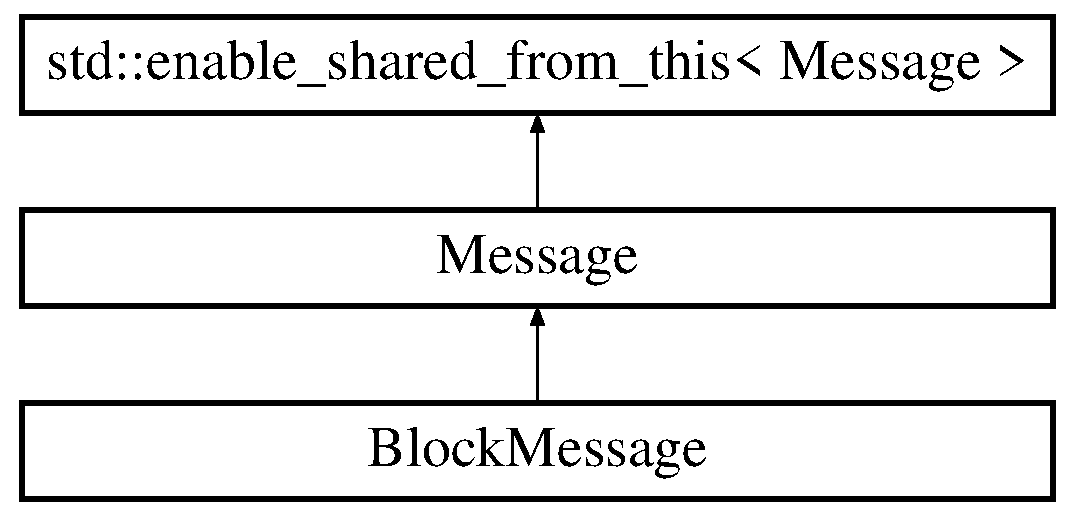
\includegraphics[height=3.000000cm]{classBlockMessage}
\end{center}
\end{figure}
\subsection*{Public Member Functions}
\begin{DoxyCompactItemize}
\item 
\mbox{\hyperlink{classBlockMessage_aac9856415dfd620f66e669e119e04af2}{Block\+Message}} (std\+::shared\+\_\+ptr$<$ \mbox{\hyperlink{classBlock}{Block}} $>$ block\+Ptr)
\item 
\mbox{\hyperlink{classBlockMessage_a8c3d6ddc50c03e4e9ddf22bead092dec}{Block\+Message}} (rapidjson\+::\+Document $\ast$doc)
\item 
rapidjson\+::\+Value \mbox{\hyperlink{classBlockMessage_afe33ddfdae83a25d98dd28541bc2fcfe}{json}} (rapidjson\+::\+Document $\ast$document) const override
\end{DoxyCompactItemize}
\subsection*{Private Attributes}
\begin{DoxyCompactItemize}
\item 
std\+::shared\+\_\+ptr$<$ \mbox{\hyperlink{classBlock}{Block}} $>$ \mbox{\hyperlink{classBlockMessage_a546ae4b4e006de9e2776f4f2a40f3b9d}{block}}
\end{DoxyCompactItemize}
\subsection*{Additional Inherited Members}


\subsection{Constructor \& Destructor Documentation}
\mbox{\Hypertarget{classBlockMessage_aac9856415dfd620f66e669e119e04af2}\label{classBlockMessage_aac9856415dfd620f66e669e119e04af2}} 
\index{Block\+Message@{Block\+Message}!Block\+Message@{Block\+Message}}
\index{Block\+Message@{Block\+Message}!Block\+Message@{Block\+Message}}
\subsubsection{\texorpdfstring{Block\+Message()}{BlockMessage()}\hspace{0.1cm}{\footnotesize\ttfamily [1/2]}}
{\footnotesize\ttfamily Block\+Message\+::\+Block\+Message (\begin{DoxyParamCaption}\item[{std\+::shared\+\_\+ptr$<$ \mbox{\hyperlink{classBlock}{Block}} $>$}]{block\+Ptr }\end{DoxyParamCaption})\hspace{0.3cm}{\ttfamily [explicit]}}

\mbox{\Hypertarget{classBlockMessage_a8c3d6ddc50c03e4e9ddf22bead092dec}\label{classBlockMessage_a8c3d6ddc50c03e4e9ddf22bead092dec}} 
\index{Block\+Message@{Block\+Message}!Block\+Message@{Block\+Message}}
\index{Block\+Message@{Block\+Message}!Block\+Message@{Block\+Message}}
\subsubsection{\texorpdfstring{Block\+Message()}{BlockMessage()}\hspace{0.1cm}{\footnotesize\ttfamily [2/2]}}
{\footnotesize\ttfamily Block\+Message\+::\+Block\+Message (\begin{DoxyParamCaption}\item[{rapidjson\+::\+Document $\ast$}]{doc }\end{DoxyParamCaption})\hspace{0.3cm}{\ttfamily [explicit]}}



\subsection{Member Function Documentation}
\mbox{\Hypertarget{classBlockMessage_afe33ddfdae83a25d98dd28541bc2fcfe}\label{classBlockMessage_afe33ddfdae83a25d98dd28541bc2fcfe}} 
\index{Block\+Message@{Block\+Message}!json@{json}}
\index{json@{json}!Block\+Message@{Block\+Message}}
\subsubsection{\texorpdfstring{json()}{json()}}
{\footnotesize\ttfamily rapidjson\+::\+Value Block\+Message\+::json (\begin{DoxyParamCaption}\item[{rapidjson\+::\+Document $\ast$}]{document }\end{DoxyParamCaption}) const\hspace{0.3cm}{\ttfamily [override]}, {\ttfamily [virtual]}}



Reimplemented from \mbox{\hyperlink{classMessage_a6f8e3ac2eed3a8afe9400fcd5b3447b2}{Message}}.



\subsection{Member Data Documentation}
\mbox{\Hypertarget{classBlockMessage_a546ae4b4e006de9e2776f4f2a40f3b9d}\label{classBlockMessage_a546ae4b4e006de9e2776f4f2a40f3b9d}} 
\index{Block\+Message@{Block\+Message}!block@{block}}
\index{block@{block}!Block\+Message@{Block\+Message}}
\subsubsection{\texorpdfstring{block}{block}}
{\footnotesize\ttfamily std\+::shared\+\_\+ptr$<$\mbox{\hyperlink{classBlock}{Block}}$>$ Block\+Message\+::block\hspace{0.3cm}{\ttfamily [private]}}



The documentation for this class was generated from the following files\+:\begin{DoxyCompactItemize}
\item 
include/\mbox{\hyperlink{messages_8hpp}{messages.\+hpp}}\item 
src/message/\mbox{\hyperlink{blockmessage_8cpp}{blockmessage.\+cpp}}\end{DoxyCompactItemize}

\hypertarget{classConnection}{}\section{Connection Class Reference}
\label{classConnection}\index{Connection@{Connection}}


A \mbox{\hyperlink{classConnection}{Connection}} to a peer.  




{\ttfamily \#include $<$connection.\+hpp$>$}

Inheritance diagram for Connection\+:\begin{figure}[H]
\begin{center}
\leavevmode
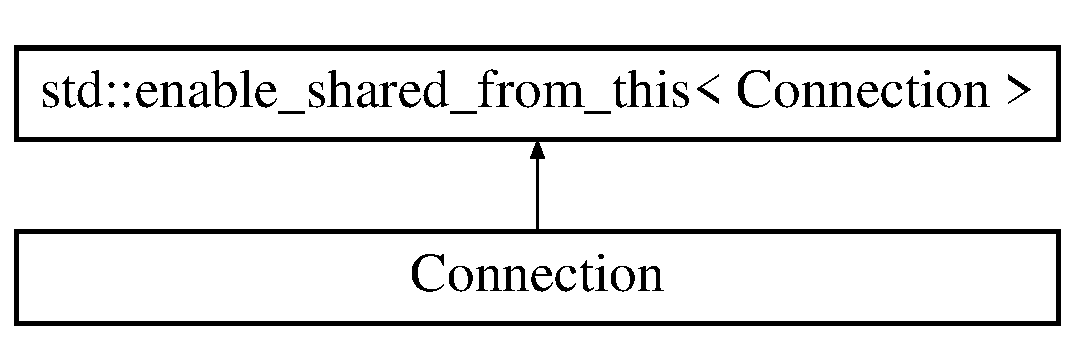
\includegraphics[height=2.000000cm]{classConnection}
\end{center}
\end{figure}
\subsection*{Public Types}
\begin{DoxyCompactItemize}
\item 
using \mbox{\hyperlink{classConnection_a1bb6cd8924ff091e9b053e3368735c9c}{pointer}} = std\+::shared\+\_\+ptr$<$ \mbox{\hyperlink{classConnection}{Connection}} $>$
\end{DoxyCompactItemize}
\subsection*{Public Member Functions}
\begin{DoxyCompactItemize}
\item 
std\+::string \mbox{\hyperlink{classConnection_ae1d2f498761143716cc12fdc76b46203}{remote}} () const
\begin{DoxyCompactList}\small\item\em IP Adress of remote connection. \end{DoxyCompactList}\item 
asio\+::ip\+::tcp\+::socket \& \mbox{\hyperlink{classConnection_ac854436a3a6fdf7fdb16be04b9696447}{get\+Socket}} ()
\begin{DoxyCompactList}\small\item\em Reference to the socket. \end{DoxyCompactList}\item 
void \mbox{\hyperlink{classConnection_a47c25a31352a71e2a6902d37fc5fa2ba}{start}} ()
\begin{DoxyCompactList}\small\item\em Initial state of \mbox{\hyperlink{classConnection}{Connection}}. \end{DoxyCompactList}\item 
void \mbox{\hyperlink{classConnection_ad8fa49332af5ccc42768f94bdf711187}{send\+Message}} (\mbox{\hyperlink{classMessage_a3f7f2aa1058cb5f0b74a1fbb7fcd00e5}{Message\+::message\+Pointer}} message)
\begin{DoxyCompactList}\small\item\em Send a \mbox{\hyperlink{classMessage}{Message}}. \end{DoxyCompactList}\item 
void \mbox{\hyperlink{classConnection_a765fb34abf97d31b9c2c49e1e1c76a00}{bind}} (asio\+::ip\+::address address)
\begin{DoxyCompactList}\small\item\em Connect to a remote address. \end{DoxyCompactList}\item 
void \mbox{\hyperlink{classConnection_a4f79c85d33fd0a9e640405ec665cc01d}{idle}} ()
\begin{DoxyCompactList}\small\item\em Idle loop of the \mbox{\hyperlink{classConnection}{Connection}}. \end{DoxyCompactList}\item 
void \mbox{\hyperlink{classConnection_a2e12f0ca3e66692c1bc3ad858dfa2d4e}{wave}} ()
\begin{DoxyCompactList}\small\item\em Exchange of \mbox{\hyperlink{classWhoAmI}{Who\+AmI}}. \end{DoxyCompactList}\end{DoxyCompactItemize}
\subsection*{Static Public Member Functions}
\begin{DoxyCompactItemize}
\item 
static \mbox{\hyperlink{classConnection_a1bb6cd8924ff091e9b053e3368735c9c}{pointer}} \mbox{\hyperlink{classConnection_a31f4b3c4ce970776f98b5fb20bdf3ef1}{create}} (asio\+::io\+\_\+context \&io\+\_\+context, \mbox{\hyperlink{classNode}{Node}} $\ast$\mbox{\hyperlink{classConnection_a0e90a6ef9361901f3d7c25e00d0a2016}{node}})
\begin{DoxyCompactList}\small\item\em Creates a shared\+\_\+ptr of \mbox{\hyperlink{classConnection}{Connection}}. \end{DoxyCompactList}\end{DoxyCompactItemize}
\subsection*{Private Member Functions}
\begin{DoxyCompactItemize}
\item 
\mbox{\hyperlink{classConnection_a0679a72f407a3c3fca0cea1cd2cd9eda}{Connection}} (asio\+::io\+\_\+context \&io\+\_\+context, \mbox{\hyperlink{classNode}{Node}} $\ast$\mbox{\hyperlink{classConnection_a0e90a6ef9361901f3d7c25e00d0a2016}{node}})
\item 
void \mbox{\hyperlink{classConnection_af084bfb2043337222d885cc8cc46201d}{handle\+Read}} ()
\begin{DoxyCompactList}\small\item\em Called when reading a \mbox{\hyperlink{classMessage}{Message}}. \end{DoxyCompactList}\item 
void \mbox{\hyperlink{classConnection_a0b08401c5769b84c2a2b4b99363925fa}{handle\+Write}} (std\+::string type)
\begin{DoxyCompactList}\small\item\em Called when writing a \mbox{\hyperlink{classMessage}{Message}}. \end{DoxyCompactList}\item 
void \mbox{\hyperlink{classConnection_a489def548f673328fe383c5625224367}{reset\+Buffer}} ()
\end{DoxyCompactItemize}
\subsection*{Private Attributes}
\begin{DoxyCompactItemize}
\item 
asio\+::ip\+::tcp\+::socket \mbox{\hyperlink{classConnection_a8b4cf76de02e4eaa6a2afdc65c42cfdc}{socket}}
\item 
\mbox{\hyperlink{classNode}{Node}} $\ast$ \mbox{\hyperlink{classConnection_a0e90a6ef9361901f3d7c25e00d0a2016}{node}}
\item 
bool \mbox{\hyperlink{classConnection_ac8ec569c3d8e883446c1498d6b0fa425}{waved}}
\begin{DoxyCompactList}\small\item\em has the node send a \mbox{\hyperlink{classWhoAmI}{Who\+AmI}} \end{DoxyCompactList}\item 
bool \mbox{\hyperlink{classConnection_a1445f1ca4d7fd2155a7de480340b370a}{connected}}
\begin{DoxyCompactList}\small\item\em recieved a \mbox{\hyperlink{classWhoAmI}{Who\+AmI}} \end{DoxyCompactList}\item 
std\+::vector$<$ \mbox{\hyperlink{classMessage_a3f7f2aa1058cb5f0b74a1fbb7fcd00e5}{Message\+::message\+Pointer}} $>$ \mbox{\hyperlink{classConnection_ad5f7e4d6f209106c33e9e996a0c49932}{buffered\+Messages}}
\begin{DoxyCompactList}\small\item\em \mbox{\hyperlink{classMessage}{Message}} buffered before \mbox{\hyperlink{classWhoAmI}{Who\+AmI}} exchange. \end{DoxyCompactList}\item 
asio\+::streambuf \mbox{\hyperlink{classConnection_a99e0a006406f126fc4c538ba71532397}{buffer}}
\end{DoxyCompactItemize}


\subsection{Detailed Description}
A \mbox{\hyperlink{classConnection}{Connection}} to a peer. 

\subsection{Member Typedef Documentation}
\mbox{\Hypertarget{classConnection_a1bb6cd8924ff091e9b053e3368735c9c}\label{classConnection_a1bb6cd8924ff091e9b053e3368735c9c}} 
\index{Connection@{Connection}!pointer@{pointer}}
\index{pointer@{pointer}!Connection@{Connection}}
\subsubsection{\texorpdfstring{pointer}{pointer}}
{\footnotesize\ttfamily using \mbox{\hyperlink{classConnection_a1bb6cd8924ff091e9b053e3368735c9c}{Connection\+::pointer}} =  std\+::shared\+\_\+ptr$<$\mbox{\hyperlink{classConnection}{Connection}}$>$}



\subsection{Constructor \& Destructor Documentation}
\mbox{\Hypertarget{classConnection_a0679a72f407a3c3fca0cea1cd2cd9eda}\label{classConnection_a0679a72f407a3c3fca0cea1cd2cd9eda}} 
\index{Connection@{Connection}!Connection@{Connection}}
\index{Connection@{Connection}!Connection@{Connection}}
\subsubsection{\texorpdfstring{Connection()}{Connection()}}
{\footnotesize\ttfamily Connection\+::\+Connection (\begin{DoxyParamCaption}\item[{asio\+::io\+\_\+context \&}]{io\+\_\+context,  }\item[{\mbox{\hyperlink{classNode}{Node}} $\ast$}]{node }\end{DoxyParamCaption})\hspace{0.3cm}{\ttfamily [private]}}



\subsection{Member Function Documentation}
\mbox{\Hypertarget{classConnection_a765fb34abf97d31b9c2c49e1e1c76a00}\label{classConnection_a765fb34abf97d31b9c2c49e1e1c76a00}} 
\index{Connection@{Connection}!bind@{bind}}
\index{bind@{bind}!Connection@{Connection}}
\subsubsection{\texorpdfstring{bind()}{bind()}}
{\footnotesize\ttfamily void Connection\+::bind (\begin{DoxyParamCaption}\item[{asio\+::ip\+::address}]{address }\end{DoxyParamCaption})}



Connect to a remote address. 


\begin{DoxyParams}{Parameters}
{\em address} & IP address to connect to \\
\hline
\end{DoxyParams}
\mbox{\Hypertarget{classConnection_a31f4b3c4ce970776f98b5fb20bdf3ef1}\label{classConnection_a31f4b3c4ce970776f98b5fb20bdf3ef1}} 
\index{Connection@{Connection}!create@{create}}
\index{create@{create}!Connection@{Connection}}
\subsubsection{\texorpdfstring{create()}{create()}}
{\footnotesize\ttfamily \mbox{\hyperlink{classConnection_a1bb6cd8924ff091e9b053e3368735c9c}{Connection\+::pointer}} Connection\+::create (\begin{DoxyParamCaption}\item[{asio\+::io\+\_\+context \&}]{io\+\_\+context,  }\item[{\mbox{\hyperlink{classNode}{Node}} $\ast$}]{node }\end{DoxyParamCaption})\hspace{0.3cm}{\ttfamily [static]}}



Creates a shared\+\_\+ptr of \mbox{\hyperlink{classConnection}{Connection}}. 


\begin{DoxyParams}{Parameters}
{\em io\+\_\+context} & io\+\_\+context for async operation \\
\hline
{\em node} & pointer to a \mbox{\hyperlink{classNode}{Node}} to handle actions \\
\hline
\end{DoxyParams}
\mbox{\Hypertarget{classConnection_ac854436a3a6fdf7fdb16be04b9696447}\label{classConnection_ac854436a3a6fdf7fdb16be04b9696447}} 
\index{Connection@{Connection}!get\+Socket@{get\+Socket}}
\index{get\+Socket@{get\+Socket}!Connection@{Connection}}
\subsubsection{\texorpdfstring{get\+Socket()}{getSocket()}}
{\footnotesize\ttfamily asio\+::ip\+::tcp\+::socket \& Connection\+::get\+Socket (\begin{DoxyParamCaption}{ }\end{DoxyParamCaption})}



Reference to the socket. 

\mbox{\Hypertarget{classConnection_af084bfb2043337222d885cc8cc46201d}\label{classConnection_af084bfb2043337222d885cc8cc46201d}} 
\index{Connection@{Connection}!handle\+Read@{handle\+Read}}
\index{handle\+Read@{handle\+Read}!Connection@{Connection}}
\subsubsection{\texorpdfstring{handle\+Read()}{handleRead()}}
{\footnotesize\ttfamily void Connection\+::handle\+Read (\begin{DoxyParamCaption}{ }\end{DoxyParamCaption})\hspace{0.3cm}{\ttfamily [private]}}



Called when reading a \mbox{\hyperlink{classMessage}{Message}}. 

\mbox{\Hypertarget{classConnection_a0b08401c5769b84c2a2b4b99363925fa}\label{classConnection_a0b08401c5769b84c2a2b4b99363925fa}} 
\index{Connection@{Connection}!handle\+Write@{handle\+Write}}
\index{handle\+Write@{handle\+Write}!Connection@{Connection}}
\subsubsection{\texorpdfstring{handle\+Write()}{handleWrite()}}
{\footnotesize\ttfamily void Connection\+::handle\+Write (\begin{DoxyParamCaption}\item[{std\+::string}]{type }\end{DoxyParamCaption})\hspace{0.3cm}{\ttfamily [private]}}



Called when writing a \mbox{\hyperlink{classMessage}{Message}}. 

\mbox{\Hypertarget{classConnection_a4f79c85d33fd0a9e640405ec665cc01d}\label{classConnection_a4f79c85d33fd0a9e640405ec665cc01d}} 
\index{Connection@{Connection}!idle@{idle}}
\index{idle@{idle}!Connection@{Connection}}
\subsubsection{\texorpdfstring{idle()}{idle()}}
{\footnotesize\ttfamily void Connection\+::idle (\begin{DoxyParamCaption}{ }\end{DoxyParamCaption})}



Idle loop of the \mbox{\hyperlink{classConnection}{Connection}}. 

\mbox{\Hypertarget{classConnection_ae1d2f498761143716cc12fdc76b46203}\label{classConnection_ae1d2f498761143716cc12fdc76b46203}} 
\index{Connection@{Connection}!remote@{remote}}
\index{remote@{remote}!Connection@{Connection}}
\subsubsection{\texorpdfstring{remote()}{remote()}}
{\footnotesize\ttfamily std\+::string Connection\+::remote (\begin{DoxyParamCaption}{ }\end{DoxyParamCaption}) const}



IP Adress of remote connection. 

\mbox{\Hypertarget{classConnection_a489def548f673328fe383c5625224367}\label{classConnection_a489def548f673328fe383c5625224367}} 
\index{Connection@{Connection}!reset\+Buffer@{reset\+Buffer}}
\index{reset\+Buffer@{reset\+Buffer}!Connection@{Connection}}
\subsubsection{\texorpdfstring{reset\+Buffer()}{resetBuffer()}}
{\footnotesize\ttfamily void Connection\+::reset\+Buffer (\begin{DoxyParamCaption}{ }\end{DoxyParamCaption})\hspace{0.3cm}{\ttfamily [private]}}

\mbox{\Hypertarget{classConnection_ad8fa49332af5ccc42768f94bdf711187}\label{classConnection_ad8fa49332af5ccc42768f94bdf711187}} 
\index{Connection@{Connection}!send\+Message@{send\+Message}}
\index{send\+Message@{send\+Message}!Connection@{Connection}}
\subsubsection{\texorpdfstring{send\+Message()}{sendMessage()}}
{\footnotesize\ttfamily void Connection\+::send\+Message (\begin{DoxyParamCaption}\item[{\mbox{\hyperlink{classMessage_a3f7f2aa1058cb5f0b74a1fbb7fcd00e5}{Message\+::message\+Pointer}}}]{message }\end{DoxyParamCaption})}



Send a \mbox{\hyperlink{classMessage}{Message}}. 


\begin{DoxyParams}{Parameters}
{\em message} & shared\+\_\+ptr of a \mbox{\hyperlink{classMessage}{Message}} \\
\hline
\end{DoxyParams}
\mbox{\Hypertarget{classConnection_a47c25a31352a71e2a6902d37fc5fa2ba}\label{classConnection_a47c25a31352a71e2a6902d37fc5fa2ba}} 
\index{Connection@{Connection}!start@{start}}
\index{start@{start}!Connection@{Connection}}
\subsubsection{\texorpdfstring{start()}{start()}}
{\footnotesize\ttfamily void Connection\+::start (\begin{DoxyParamCaption}{ }\end{DoxyParamCaption})}



Initial state of \mbox{\hyperlink{classConnection}{Connection}}. 

\mbox{\Hypertarget{classConnection_a2e12f0ca3e66692c1bc3ad858dfa2d4e}\label{classConnection_a2e12f0ca3e66692c1bc3ad858dfa2d4e}} 
\index{Connection@{Connection}!wave@{wave}}
\index{wave@{wave}!Connection@{Connection}}
\subsubsection{\texorpdfstring{wave()}{wave()}}
{\footnotesize\ttfamily void Connection\+::wave (\begin{DoxyParamCaption}{ }\end{DoxyParamCaption})}



Exchange of \mbox{\hyperlink{classWhoAmI}{Who\+AmI}}. 



\subsection{Member Data Documentation}
\mbox{\Hypertarget{classConnection_a99e0a006406f126fc4c538ba71532397}\label{classConnection_a99e0a006406f126fc4c538ba71532397}} 
\index{Connection@{Connection}!buffer@{buffer}}
\index{buffer@{buffer}!Connection@{Connection}}
\subsubsection{\texorpdfstring{buffer}{buffer}}
{\footnotesize\ttfamily asio\+::streambuf Connection\+::buffer\hspace{0.3cm}{\ttfamily [private]}}

\mbox{\Hypertarget{classConnection_ad5f7e4d6f209106c33e9e996a0c49932}\label{classConnection_ad5f7e4d6f209106c33e9e996a0c49932}} 
\index{Connection@{Connection}!buffered\+Messages@{buffered\+Messages}}
\index{buffered\+Messages@{buffered\+Messages}!Connection@{Connection}}
\subsubsection{\texorpdfstring{buffered\+Messages}{bufferedMessages}}
{\footnotesize\ttfamily std\+::vector$<$\mbox{\hyperlink{classMessage_a3f7f2aa1058cb5f0b74a1fbb7fcd00e5}{Message\+::message\+Pointer}}$>$ Connection\+::buffered\+Messages\hspace{0.3cm}{\ttfamily [private]}}



\mbox{\hyperlink{classMessage}{Message}} buffered before \mbox{\hyperlink{classWhoAmI}{Who\+AmI}} exchange. 

\mbox{\Hypertarget{classConnection_a1445f1ca4d7fd2155a7de480340b370a}\label{classConnection_a1445f1ca4d7fd2155a7de480340b370a}} 
\index{Connection@{Connection}!connected@{connected}}
\index{connected@{connected}!Connection@{Connection}}
\subsubsection{\texorpdfstring{connected}{connected}}
{\footnotesize\ttfamily bool Connection\+::connected\hspace{0.3cm}{\ttfamily [private]}}



recieved a \mbox{\hyperlink{classWhoAmI}{Who\+AmI}} 

\mbox{\Hypertarget{classConnection_a0e90a6ef9361901f3d7c25e00d0a2016}\label{classConnection_a0e90a6ef9361901f3d7c25e00d0a2016}} 
\index{Connection@{Connection}!node@{node}}
\index{node@{node}!Connection@{Connection}}
\subsubsection{\texorpdfstring{node}{node}}
{\footnotesize\ttfamily \mbox{\hyperlink{classNode}{Node}}$\ast$ Connection\+::node\hspace{0.3cm}{\ttfamily [private]}}

\mbox{\Hypertarget{classConnection_a8b4cf76de02e4eaa6a2afdc65c42cfdc}\label{classConnection_a8b4cf76de02e4eaa6a2afdc65c42cfdc}} 
\index{Connection@{Connection}!socket@{socket}}
\index{socket@{socket}!Connection@{Connection}}
\subsubsection{\texorpdfstring{socket}{socket}}
{\footnotesize\ttfamily asio\+::ip\+::tcp\+::socket Connection\+::socket\hspace{0.3cm}{\ttfamily [private]}}

\mbox{\Hypertarget{classConnection_ac8ec569c3d8e883446c1498d6b0fa425}\label{classConnection_ac8ec569c3d8e883446c1498d6b0fa425}} 
\index{Connection@{Connection}!waved@{waved}}
\index{waved@{waved}!Connection@{Connection}}
\subsubsection{\texorpdfstring{waved}{waved}}
{\footnotesize\ttfamily bool Connection\+::waved\hspace{0.3cm}{\ttfamily [private]}}



has the node send a \mbox{\hyperlink{classWhoAmI}{Who\+AmI}} 



The documentation for this class was generated from the following files\+:\begin{DoxyCompactItemize}
\item 
include/\mbox{\hyperlink{connection_8hpp}{connection.\+hpp}}\item 
src/\mbox{\hyperlink{connection_8cpp}{connection.\+cpp}}\end{DoxyCompactItemize}

\hypertarget{classECDSASignature}{}\section{E\+C\+D\+S\+A\+Signature Class Reference}
\label{classECDSASignature}\index{E\+C\+D\+S\+A\+Signature@{E\+C\+D\+S\+A\+Signature}}


Signatures using secp256k1.  




{\ttfamily \#include $<$crypto.\+hpp$>$}

\subsection*{Public Member Functions}
\begin{DoxyCompactItemize}
\item 
\mbox{\hyperlink{classECDSASignature_a9b02f26402e6e70ef8fa80f799652c27}{E\+C\+D\+S\+A\+Signature}} (std\+::string encoded\+Signature)
\begin{DoxyCompactList}\small\item\em Construct a \mbox{\hyperlink{classECDSASignature}{E\+C\+D\+S\+A\+Signature}} from signature. \end{DoxyCompactList}\item 
\mbox{\hyperlink{classECDSASignature_a459b85f89b2d2706cac10c8f28298e9b}{E\+C\+D\+S\+A\+Signature}} (std\+::string message, e\+Curve\+::\+Private\+Key private\+Key)
\begin{DoxyCompactList}\small\item\em Construct a \mbox{\hyperlink{classECDSASignature}{E\+C\+D\+S\+A\+Signature}} to sign a string. \end{DoxyCompactList}\item 
std\+::string \mbox{\hyperlink{classECDSASignature_a9179c6cec311dbb746ffe876dce12844}{hex}} () const
\begin{DoxyCompactList}\small\item\em Hex representation of signature. \end{DoxyCompactList}\item 
bool \mbox{\hyperlink{classECDSASignature_aae4f75f7c0b41adddee0123392d8d960}{verify}} (std\+::string message, std\+::string public\+Key\+String) const
\begin{DoxyCompactList}\small\item\em verifies if a message is signed \end{DoxyCompactList}\end{DoxyCompactItemize}
\subsection*{Private Attributes}
\begin{DoxyCompactItemize}
\item 
std\+::string \mbox{\hyperlink{classECDSASignature_aae4afcd90bbe797c9c60fb6967dd0849}{signature}}
\begin{DoxyCompactList}\small\item\em A binary string signature. \end{DoxyCompactList}\end{DoxyCompactItemize}


\subsection{Detailed Description}
Signatures using secp256k1. 

\subsection{Constructor \& Destructor Documentation}
\mbox{\Hypertarget{classECDSASignature_a9b02f26402e6e70ef8fa80f799652c27}\label{classECDSASignature_a9b02f26402e6e70ef8fa80f799652c27}} 
\index{E\+C\+D\+S\+A\+Signature@{E\+C\+D\+S\+A\+Signature}!E\+C\+D\+S\+A\+Signature@{E\+C\+D\+S\+A\+Signature}}
\index{E\+C\+D\+S\+A\+Signature@{E\+C\+D\+S\+A\+Signature}!E\+C\+D\+S\+A\+Signature@{E\+C\+D\+S\+A\+Signature}}
\subsubsection{\texorpdfstring{E\+C\+D\+S\+A\+Signature()}{ECDSASignature()}\hspace{0.1cm}{\footnotesize\ttfamily [1/2]}}
{\footnotesize\ttfamily E\+C\+D\+S\+A\+Signature\+::\+E\+C\+D\+S\+A\+Signature (\begin{DoxyParamCaption}\item[{std\+::string}]{encoded\+Signature }\end{DoxyParamCaption})}



Construct a \mbox{\hyperlink{classECDSASignature}{E\+C\+D\+S\+A\+Signature}} from signature. 


\begin{DoxyParams}{Parameters}
{\em encoded\+Signature} & signature as hex representation \\
\hline
\end{DoxyParams}
\mbox{\Hypertarget{classECDSASignature_a459b85f89b2d2706cac10c8f28298e9b}\label{classECDSASignature_a459b85f89b2d2706cac10c8f28298e9b}} 
\index{E\+C\+D\+S\+A\+Signature@{E\+C\+D\+S\+A\+Signature}!E\+C\+D\+S\+A\+Signature@{E\+C\+D\+S\+A\+Signature}}
\index{E\+C\+D\+S\+A\+Signature@{E\+C\+D\+S\+A\+Signature}!E\+C\+D\+S\+A\+Signature@{E\+C\+D\+S\+A\+Signature}}
\subsubsection{\texorpdfstring{E\+C\+D\+S\+A\+Signature()}{ECDSASignature()}\hspace{0.1cm}{\footnotesize\ttfamily [2/2]}}
{\footnotesize\ttfamily E\+C\+D\+S\+A\+Signature\+::\+E\+C\+D\+S\+A\+Signature (\begin{DoxyParamCaption}\item[{std\+::string}]{message,  }\item[{e\+Curve\+::\+Private\+Key}]{private\+Key }\end{DoxyParamCaption})}



Construct a \mbox{\hyperlink{classECDSASignature}{E\+C\+D\+S\+A\+Signature}} to sign a string. 


\begin{DoxyParams}{Parameters}
{\em message} & a string to be signed \\
\hline
{\em private\+Key} & a secp256k1 private key \\
\hline
\end{DoxyParams}


\subsection{Member Function Documentation}
\mbox{\Hypertarget{classECDSASignature_a9179c6cec311dbb746ffe876dce12844}\label{classECDSASignature_a9179c6cec311dbb746ffe876dce12844}} 
\index{E\+C\+D\+S\+A\+Signature@{E\+C\+D\+S\+A\+Signature}!hex@{hex}}
\index{hex@{hex}!E\+C\+D\+S\+A\+Signature@{E\+C\+D\+S\+A\+Signature}}
\subsubsection{\texorpdfstring{hex()}{hex()}}
{\footnotesize\ttfamily std\+::string E\+C\+D\+S\+A\+Signature\+::hex (\begin{DoxyParamCaption}{ }\end{DoxyParamCaption}) const}



Hex representation of signature. 

\mbox{\Hypertarget{classECDSASignature_aae4f75f7c0b41adddee0123392d8d960}\label{classECDSASignature_aae4f75f7c0b41adddee0123392d8d960}} 
\index{E\+C\+D\+S\+A\+Signature@{E\+C\+D\+S\+A\+Signature}!verify@{verify}}
\index{verify@{verify}!E\+C\+D\+S\+A\+Signature@{E\+C\+D\+S\+A\+Signature}}
\subsubsection{\texorpdfstring{verify()}{verify()}}
{\footnotesize\ttfamily bool E\+C\+D\+S\+A\+Signature\+::verify (\begin{DoxyParamCaption}\item[{std\+::string}]{message,  }\item[{std\+::string}]{public\+Key\+String }\end{DoxyParamCaption}) const}



verifies if a message is signed 


\begin{DoxyParams}{Parameters}
{\em message} & string to be verified \\
\hline
{\em public\+Key\+String} & Hex reprensation of public the public key for checking with \\
\hline
\end{DoxyParams}


\subsection{Member Data Documentation}
\mbox{\Hypertarget{classECDSASignature_aae4afcd90bbe797c9c60fb6967dd0849}\label{classECDSASignature_aae4afcd90bbe797c9c60fb6967dd0849}} 
\index{E\+C\+D\+S\+A\+Signature@{E\+C\+D\+S\+A\+Signature}!signature@{signature}}
\index{signature@{signature}!E\+C\+D\+S\+A\+Signature@{E\+C\+D\+S\+A\+Signature}}
\subsubsection{\texorpdfstring{signature}{signature}}
{\footnotesize\ttfamily std\+::string E\+C\+D\+S\+A\+Signature\+::signature\hspace{0.3cm}{\ttfamily [private]}}



A binary string signature. 



The documentation for this class was generated from the following files\+:\begin{DoxyCompactItemize}
\item 
include/\mbox{\hyperlink{crypto_8hpp}{crypto.\+hpp}}\item 
src/\mbox{\hyperlink{crypto_8cpp}{crypto.\+cpp}}\end{DoxyCompactItemize}

\hypertarget{classGetBlocks}{}\section{Get\+Blocks Class Reference}
\label{classGetBlocks}\index{Get\+Blocks@{Get\+Blocks}}


{\ttfamily \#include $<$messages.\+hpp$>$}

Inheritance diagram for Get\+Blocks\+:\begin{figure}[H]
\begin{center}
\leavevmode
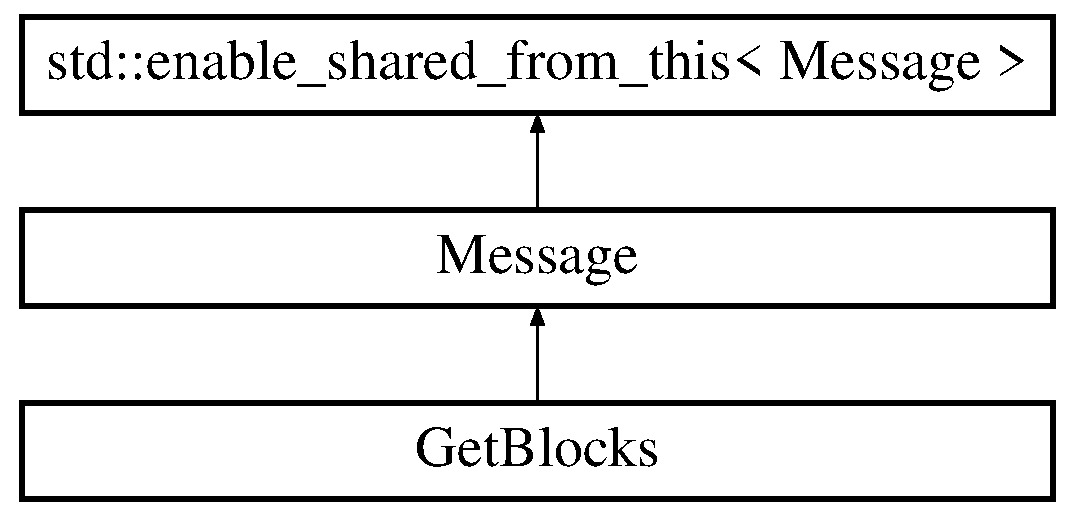
\includegraphics[height=3.000000cm]{classGetBlocks}
\end{center}
\end{figure}
\subsection*{Public Member Functions}
\begin{DoxyCompactItemize}
\item 
\mbox{\hyperlink{classGetBlocks_aec0906bd19989a7982cad0aefc3d750a}{Get\+Blocks}} (std\+::vector$<$ std\+::string $>$ hash\+List, std\+::string stop\+Hash\+String)
\item 
\mbox{\hyperlink{classGetBlocks_a0ce69110b775f4f122f6a20222cc0b64}{Get\+Blocks}} (rapidjson\+::\+Document $\ast$doc)
\item 
rapidjson\+::\+Value \mbox{\hyperlink{classGetBlocks_a8b77916e999ba0a730e31b90b4733928}{json}} (rapidjson\+::\+Document $\ast$doc) const override
\end{DoxyCompactItemize}
\subsection*{Private Attributes}
\begin{DoxyCompactItemize}
\item 
std\+::vector$<$ std\+::string $>$ \mbox{\hyperlink{classGetBlocks_a24b217db1c15cdfcd91fbebf2b10238a}{block\+Hashes}}
\item 
std\+::string \mbox{\hyperlink{classGetBlocks_a7b367127191d3855f593dc7b96188853}{stop\+Hash}}
\end{DoxyCompactItemize}
\subsection*{Additional Inherited Members}


\subsection{Constructor \& Destructor Documentation}
\mbox{\Hypertarget{classGetBlocks_aec0906bd19989a7982cad0aefc3d750a}\label{classGetBlocks_aec0906bd19989a7982cad0aefc3d750a}} 
\index{Get\+Blocks@{Get\+Blocks}!Get\+Blocks@{Get\+Blocks}}
\index{Get\+Blocks@{Get\+Blocks}!Get\+Blocks@{Get\+Blocks}}
\subsubsection{\texorpdfstring{Get\+Blocks()}{GetBlocks()}\hspace{0.1cm}{\footnotesize\ttfamily [1/2]}}
{\footnotesize\ttfamily Get\+Blocks\+::\+Get\+Blocks (\begin{DoxyParamCaption}\item[{std\+::vector$<$ std\+::string $>$}]{hash\+List,  }\item[{std\+::string}]{stop\+Hash\+String }\end{DoxyParamCaption})}

\mbox{\Hypertarget{classGetBlocks_a0ce69110b775f4f122f6a20222cc0b64}\label{classGetBlocks_a0ce69110b775f4f122f6a20222cc0b64}} 
\index{Get\+Blocks@{Get\+Blocks}!Get\+Blocks@{Get\+Blocks}}
\index{Get\+Blocks@{Get\+Blocks}!Get\+Blocks@{Get\+Blocks}}
\subsubsection{\texorpdfstring{Get\+Blocks()}{GetBlocks()}\hspace{0.1cm}{\footnotesize\ttfamily [2/2]}}
{\footnotesize\ttfamily Get\+Blocks\+::\+Get\+Blocks (\begin{DoxyParamCaption}\item[{rapidjson\+::\+Document $\ast$}]{doc }\end{DoxyParamCaption})\hspace{0.3cm}{\ttfamily [explicit]}}



\subsection{Member Function Documentation}
\mbox{\Hypertarget{classGetBlocks_a8b77916e999ba0a730e31b90b4733928}\label{classGetBlocks_a8b77916e999ba0a730e31b90b4733928}} 
\index{Get\+Blocks@{Get\+Blocks}!json@{json}}
\index{json@{json}!Get\+Blocks@{Get\+Blocks}}
\subsubsection{\texorpdfstring{json()}{json()}}
{\footnotesize\ttfamily rapidjson\+::\+Value Get\+Blocks\+::json (\begin{DoxyParamCaption}\item[{rapidjson\+::\+Document $\ast$}]{doc }\end{DoxyParamCaption}) const\hspace{0.3cm}{\ttfamily [override]}, {\ttfamily [virtual]}}



Reimplemented from \mbox{\hyperlink{classMessage_a6f8e3ac2eed3a8afe9400fcd5b3447b2}{Message}}.



\subsection{Member Data Documentation}
\mbox{\Hypertarget{classGetBlocks_a24b217db1c15cdfcd91fbebf2b10238a}\label{classGetBlocks_a24b217db1c15cdfcd91fbebf2b10238a}} 
\index{Get\+Blocks@{Get\+Blocks}!block\+Hashes@{block\+Hashes}}
\index{block\+Hashes@{block\+Hashes}!Get\+Blocks@{Get\+Blocks}}
\subsubsection{\texorpdfstring{block\+Hashes}{blockHashes}}
{\footnotesize\ttfamily std\+::vector$<$ std\+::string $>$ Get\+Blocks\+::block\+Hashes\hspace{0.3cm}{\ttfamily [private]}}

\mbox{\Hypertarget{classGetBlocks_a7b367127191d3855f593dc7b96188853}\label{classGetBlocks_a7b367127191d3855f593dc7b96188853}} 
\index{Get\+Blocks@{Get\+Blocks}!stop\+Hash@{stop\+Hash}}
\index{stop\+Hash@{stop\+Hash}!Get\+Blocks@{Get\+Blocks}}
\subsubsection{\texorpdfstring{stop\+Hash}{stopHash}}
{\footnotesize\ttfamily std\+::string Get\+Blocks\+::stop\+Hash\hspace{0.3cm}{\ttfamily [private]}}



The documentation for this class was generated from the following files\+:\begin{DoxyCompactItemize}
\item 
include/\mbox{\hyperlink{messages_8hpp}{messages.\+hpp}}\item 
src/message/\mbox{\hyperlink{getblocks_8cpp}{getblocks.\+cpp}}\end{DoxyCompactItemize}

\hypertarget{classGetData}{}\section{Get\+Data Class Reference}
\label{classGetData}\index{Get\+Data@{Get\+Data}}


{\ttfamily \#include $<$messages.\+hpp$>$}

Inheritance diagram for Get\+Data\+:\begin{figure}[H]
\begin{center}
\leavevmode
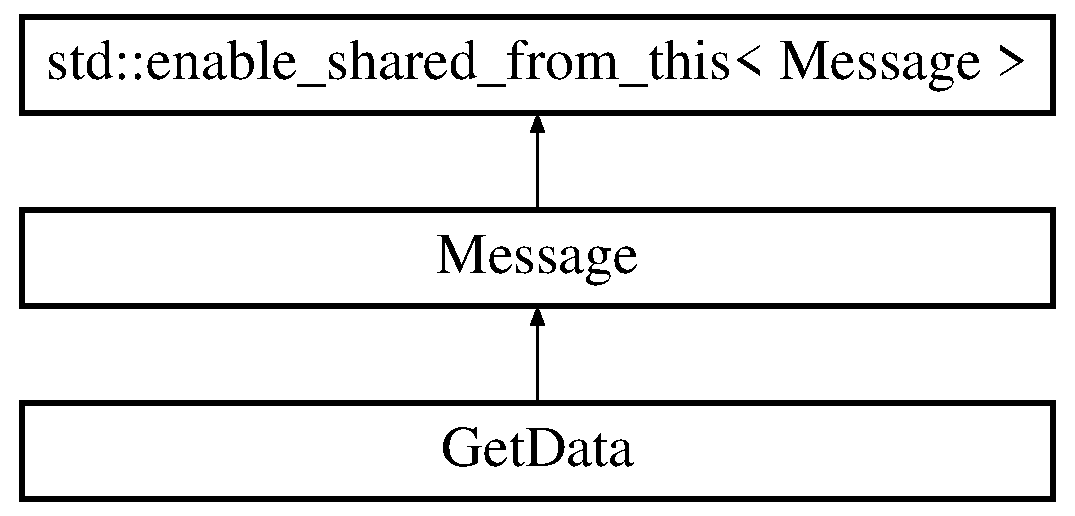
\includegraphics[height=3.000000cm]{classGetData}
\end{center}
\end{figure}
\subsection*{Public Member Functions}
\begin{DoxyCompactItemize}
\item 
\mbox{\hyperlink{classGetData_adb9c8dc0c3f1e40329530b26bd96f32f}{Get\+Data}} (\mbox{\hyperlink{structInvData}{Inv\+Data}} inv)
\item 
\mbox{\hyperlink{classGetData_ab1179102b6e97c85834410f0699140f6}{Get\+Data}} (rapidjson\+::\+Document $\ast$doc)
\item 
rapidjson\+::\+Value \mbox{\hyperlink{classGetData_a2fb121264fc1c5821e769f4f2389c6ff}{json}} (rapidjson\+::\+Document $\ast$document) const override
\end{DoxyCompactItemize}
\subsection*{Private Attributes}
\begin{DoxyCompactItemize}
\item 
\mbox{\hyperlink{structInvData}{Inv\+Data}} \mbox{\hyperlink{classGetData_a964b166c01dbec2325e35a62f65e504c}{inv\+Data}}
\end{DoxyCompactItemize}
\subsection*{Additional Inherited Members}


\subsection{Constructor \& Destructor Documentation}
\mbox{\Hypertarget{classGetData_adb9c8dc0c3f1e40329530b26bd96f32f}\label{classGetData_adb9c8dc0c3f1e40329530b26bd96f32f}} 
\index{Get\+Data@{Get\+Data}!Get\+Data@{Get\+Data}}
\index{Get\+Data@{Get\+Data}!Get\+Data@{Get\+Data}}
\subsubsection{\texorpdfstring{Get\+Data()}{GetData()}\hspace{0.1cm}{\footnotesize\ttfamily [1/2]}}
{\footnotesize\ttfamily Get\+Data\+::\+Get\+Data (\begin{DoxyParamCaption}\item[{\mbox{\hyperlink{structInvData}{Inv\+Data}}}]{inv }\end{DoxyParamCaption})\hspace{0.3cm}{\ttfamily [explicit]}}

\mbox{\Hypertarget{classGetData_ab1179102b6e97c85834410f0699140f6}\label{classGetData_ab1179102b6e97c85834410f0699140f6}} 
\index{Get\+Data@{Get\+Data}!Get\+Data@{Get\+Data}}
\index{Get\+Data@{Get\+Data}!Get\+Data@{Get\+Data}}
\subsubsection{\texorpdfstring{Get\+Data()}{GetData()}\hspace{0.1cm}{\footnotesize\ttfamily [2/2]}}
{\footnotesize\ttfamily Get\+Data\+::\+Get\+Data (\begin{DoxyParamCaption}\item[{rapidjson\+::\+Document $\ast$}]{doc }\end{DoxyParamCaption})\hspace{0.3cm}{\ttfamily [explicit]}}



\subsection{Member Function Documentation}
\mbox{\Hypertarget{classGetData_a2fb121264fc1c5821e769f4f2389c6ff}\label{classGetData_a2fb121264fc1c5821e769f4f2389c6ff}} 
\index{Get\+Data@{Get\+Data}!json@{json}}
\index{json@{json}!Get\+Data@{Get\+Data}}
\subsubsection{\texorpdfstring{json()}{json()}}
{\footnotesize\ttfamily rapidjson\+::\+Value Get\+Data\+::json (\begin{DoxyParamCaption}\item[{rapidjson\+::\+Document $\ast$}]{document }\end{DoxyParamCaption}) const\hspace{0.3cm}{\ttfamily [override]}, {\ttfamily [virtual]}}



Reimplemented from \mbox{\hyperlink{classMessage_a6f8e3ac2eed3a8afe9400fcd5b3447b2}{Message}}.



\subsection{Member Data Documentation}
\mbox{\Hypertarget{classGetData_a964b166c01dbec2325e35a62f65e504c}\label{classGetData_a964b166c01dbec2325e35a62f65e504c}} 
\index{Get\+Data@{Get\+Data}!inv\+Data@{inv\+Data}}
\index{inv\+Data@{inv\+Data}!Get\+Data@{Get\+Data}}
\subsubsection{\texorpdfstring{inv\+Data}{invData}}
{\footnotesize\ttfamily \mbox{\hyperlink{structInvData}{Inv\+Data}} Get\+Data\+::inv\+Data\hspace{0.3cm}{\ttfamily [private]}}



The documentation for this class was generated from the following files\+:\begin{DoxyCompactItemize}
\item 
include/\mbox{\hyperlink{messages_8hpp}{messages.\+hpp}}\item 
src/message/\mbox{\hyperlink{getdata_8cpp}{getdata.\+cpp}}\end{DoxyCompactItemize}

\hypertarget{classGetMempool}{}\section{Get\+Mempool Class Reference}
\label{classGetMempool}\index{Get\+Mempool@{Get\+Mempool}}


{\ttfamily \#include $<$messages.\+hpp$>$}

Inheritance diagram for Get\+Mempool\+:\begin{figure}[H]
\begin{center}
\leavevmode
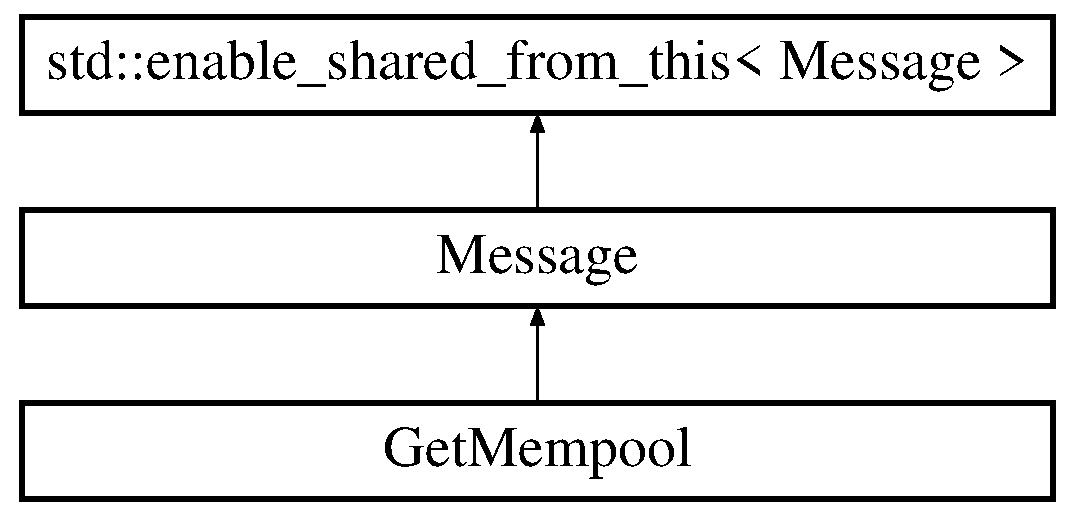
\includegraphics[height=3.000000cm]{classGetMempool}
\end{center}
\end{figure}
\subsection*{Public Member Functions}
\begin{DoxyCompactItemize}
\item 
\mbox{\hyperlink{classGetMempool_a337115b4fa5609bd3d6ae8433382ab28}{Get\+Mempool}} ()
\item 
\mbox{\hyperlink{classGetMempool_a99f4e2b501cd290d13833116aa48e0f7}{Get\+Mempool}} (rapidjson\+::\+Document $\ast$doc)
\item 
rapidjson\+::\+Value \mbox{\hyperlink{classGetMempool_a3e6fb495c609ade4e8efd3d5668c28cf}{json}} (rapidjson\+::\+Document $\ast$doc) const override
\end{DoxyCompactItemize}
\subsection*{Additional Inherited Members}


\subsection{Constructor \& Destructor Documentation}
\mbox{\Hypertarget{classGetMempool_a337115b4fa5609bd3d6ae8433382ab28}\label{classGetMempool_a337115b4fa5609bd3d6ae8433382ab28}} 
\index{Get\+Mempool@{Get\+Mempool}!Get\+Mempool@{Get\+Mempool}}
\index{Get\+Mempool@{Get\+Mempool}!Get\+Mempool@{Get\+Mempool}}
\subsubsection{\texorpdfstring{Get\+Mempool()}{GetMempool()}\hspace{0.1cm}{\footnotesize\ttfamily [1/2]}}
{\footnotesize\ttfamily Get\+Mempool\+::\+Get\+Mempool (\begin{DoxyParamCaption}{ }\end{DoxyParamCaption})}

\mbox{\Hypertarget{classGetMempool_a99f4e2b501cd290d13833116aa48e0f7}\label{classGetMempool_a99f4e2b501cd290d13833116aa48e0f7}} 
\index{Get\+Mempool@{Get\+Mempool}!Get\+Mempool@{Get\+Mempool}}
\index{Get\+Mempool@{Get\+Mempool}!Get\+Mempool@{Get\+Mempool}}
\subsubsection{\texorpdfstring{Get\+Mempool()}{GetMempool()}\hspace{0.1cm}{\footnotesize\ttfamily [2/2]}}
{\footnotesize\ttfamily Get\+Mempool\+::\+Get\+Mempool (\begin{DoxyParamCaption}\item[{rapidjson\+::\+Document $\ast$}]{doc }\end{DoxyParamCaption})\hspace{0.3cm}{\ttfamily [explicit]}}



\subsection{Member Function Documentation}
\mbox{\Hypertarget{classGetMempool_a3e6fb495c609ade4e8efd3d5668c28cf}\label{classGetMempool_a3e6fb495c609ade4e8efd3d5668c28cf}} 
\index{Get\+Mempool@{Get\+Mempool}!json@{json}}
\index{json@{json}!Get\+Mempool@{Get\+Mempool}}
\subsubsection{\texorpdfstring{json()}{json()}}
{\footnotesize\ttfamily rapidjson\+::\+Value Get\+Mempool\+::json (\begin{DoxyParamCaption}\item[{rapidjson\+::\+Document $\ast$}]{doc }\end{DoxyParamCaption}) const\hspace{0.3cm}{\ttfamily [override]}, {\ttfamily [virtual]}}



Reimplemented from \mbox{\hyperlink{classMessage_a6f8e3ac2eed3a8afe9400fcd5b3447b2}{Message}}.



The documentation for this class was generated from the following files\+:\begin{DoxyCompactItemize}
\item 
include/\mbox{\hyperlink{messages_8hpp}{messages.\+hpp}}\item 
src/message/\mbox{\hyperlink{getmempool_8cpp}{getmempool.\+cpp}}\end{DoxyCompactItemize}

\hypertarget{classHandler}{}\section{Handler Class Reference}
\label{classHandler}\index{Handler@{Handler}}


{\ttfamily \#include $<$messagehandler.\+hpp$>$}

\subsection*{Classes}
\begin{DoxyCompactItemize}
\item 
struct \mbox{\hyperlink{structHandler_1_1params}{params}}
\end{DoxyCompactItemize}
\subsection*{Static Public Member Functions}
\begin{DoxyCompactItemize}
\item 
static bool \mbox{\hyperlink{classHandler_afab4c935cf54ff1bce38c97cc4392b26}{handle}} (rapidjson\+::\+Document $\ast$doc, \mbox{\hyperlink{classNode}{Node}} $\ast$node, std\+::shared\+\_\+ptr$<$ \mbox{\hyperlink{classConnection}{Connection}} $>$ connection)
\end{DoxyCompactItemize}
\subsection*{Static Private Member Functions}
\begin{DoxyCompactItemize}
\item 
static bool \mbox{\hyperlink{classHandler_afe1ccc0e741e068b6d0c667fc421b820}{whoami}} (\mbox{\hyperlink{structHandler_1_1params}{params}} \&)
\item 
static bool \mbox{\hyperlink{classHandler_aff9b9d060534a0a09a63a4d7c1b65407}{unknown}} (\mbox{\hyperlink{structHandler_1_1params}{params}} \&, std\+::string)
\end{DoxyCompactItemize}


\subsection{Member Function Documentation}
\mbox{\Hypertarget{classHandler_afab4c935cf54ff1bce38c97cc4392b26}\label{classHandler_afab4c935cf54ff1bce38c97cc4392b26}} 
\index{Handler@{Handler}!handle@{handle}}
\index{handle@{handle}!Handler@{Handler}}
\subsubsection{\texorpdfstring{handle()}{handle()}}
{\footnotesize\ttfamily bool Handler\+::handle (\begin{DoxyParamCaption}\item[{rapidjson\+::\+Document $\ast$}]{doc,  }\item[{\mbox{\hyperlink{classNode}{Node}} $\ast$}]{node,  }\item[{std\+::shared\+\_\+ptr$<$ \mbox{\hyperlink{classConnection}{Connection}} $>$}]{connection }\end{DoxyParamCaption})\hspace{0.3cm}{\ttfamily [static]}}

\mbox{\Hypertarget{classHandler_aff9b9d060534a0a09a63a4d7c1b65407}\label{classHandler_aff9b9d060534a0a09a63a4d7c1b65407}} 
\index{Handler@{Handler}!unknown@{unknown}}
\index{unknown@{unknown}!Handler@{Handler}}
\subsubsection{\texorpdfstring{unknown()}{unknown()}}
{\footnotesize\ttfamily bool Handler\+::unknown (\begin{DoxyParamCaption}\item[{\mbox{\hyperlink{structHandler_1_1params}{params}} \&}]{p,  }\item[{std\+::string}]{unknown\+Type }\end{DoxyParamCaption})\hspace{0.3cm}{\ttfamily [static]}, {\ttfamily [private]}}

\mbox{\Hypertarget{classHandler_afe1ccc0e741e068b6d0c667fc421b820}\label{classHandler_afe1ccc0e741e068b6d0c667fc421b820}} 
\index{Handler@{Handler}!whoami@{whoami}}
\index{whoami@{whoami}!Handler@{Handler}}
\subsubsection{\texorpdfstring{whoami()}{whoami()}}
{\footnotesize\ttfamily bool Handler\+::whoami (\begin{DoxyParamCaption}\item[{\mbox{\hyperlink{structHandler_1_1params}{params}} \&}]{p }\end{DoxyParamCaption})\hspace{0.3cm}{\ttfamily [static]}, {\ttfamily [private]}}



The documentation for this class was generated from the following files\+:\begin{DoxyCompactItemize}
\item 
include/\mbox{\hyperlink{messagehandler_8hpp}{messagehandler.\+hpp}}\item 
src/\mbox{\hyperlink{messagehandler_8cpp}{messagehandler.\+cpp}}\end{DoxyCompactItemize}

\hypertarget{classHashMemory}{}\section{Hash\+Memory$<$ T $>$ Class Template Reference}
\label{classHashMemory}\index{Hash\+Memory$<$ T $>$@{Hash\+Memory$<$ T $>$}}


Wrapper around a std\+::unordered\+\_\+map.  




{\ttfamily \#include $<$hashmemory.\+hpp$>$}

\subsection*{Public Types}
\begin{DoxyCompactItemize}
\item 
using \mbox{\hyperlink{classHashMemory_ab2c7ace63d7bbcf75d523c445a3a0dbb}{pointer}} = std\+::shared\+\_\+ptr$<$ T $>$
\end{DoxyCompactItemize}
\subsection*{Public Member Functions}
\begin{DoxyCompactItemize}
\item 
bool \mbox{\hyperlink{classHashMemory_ac9bd6270bbfa924ce5f27fada28afe9f}{exists}} (std\+::string elem\+Hash) const
\begin{DoxyCompactList}\small\item\em Check existence of hash. \end{DoxyCompactList}\item 
bool \mbox{\hyperlink{classHashMemory_aca03e1a9ea9ce94e34871a004cc6f7e4}{exists}} (\mbox{\hyperlink{classHashMemory_ab2c7ace63d7bbcf75d523c445a3a0dbb}{pointer}} elem) const
\begin{DoxyCompactList}\small\item\em Check existence of object. \end{DoxyCompactList}\item 
bool \mbox{\hyperlink{classHashMemory_aa1f2e179dc50cee47891064bbb82f2c9}{add}} (\mbox{\hyperlink{classHashMemory_ab2c7ace63d7bbcf75d523c445a3a0dbb}{pointer}} element)
\begin{DoxyCompactList}\small\item\em Add element to memory. \end{DoxyCompactList}\item 
\mbox{\hyperlink{classHashMemory_ab2c7ace63d7bbcf75d523c445a3a0dbb}{pointer}} \mbox{\hyperlink{classHashMemory_a51cf6dae3ddcf94f7bf13769f6677afd}{get}} (std\+::string elem\+Hash) const
\begin{DoxyCompactList}\small\item\em Get Element (without checking) \end{DoxyCompactList}\item 
void \mbox{\hyperlink{classHashMemory_a96bcc6b0bf9ae5999ca29bb61a3eff0c}{erase}} (std\+::string elem\+Hash)
\begin{DoxyCompactList}\small\item\em Remove element (without checking) \end{DoxyCompactList}\end{DoxyCompactItemize}
\subsection*{Private Attributes}
\begin{DoxyCompactItemize}
\item 
std\+::unordered\+\_\+map$<$ std\+::string, \mbox{\hyperlink{classHashMemory_ab2c7ace63d7bbcf75d523c445a3a0dbb}{pointer}} $>$ \mbox{\hyperlink{classHashMemory_a816a44aa2d5eb7f29284856f3f27ec5f}{memory}}
\end{DoxyCompactItemize}


\subsection{Detailed Description}
\subsubsection*{template$<$class T$>$\newline
class Hash\+Memory$<$ T $>$}

Wrapper around a std\+::unordered\+\_\+map. 


\begin{DoxyTemplParams}{Template Parameters}
{\em T} & implement .hash() \\
\hline
\end{DoxyTemplParams}


\subsection{Member Typedef Documentation}
\mbox{\Hypertarget{classHashMemory_ab2c7ace63d7bbcf75d523c445a3a0dbb}\label{classHashMemory_ab2c7ace63d7bbcf75d523c445a3a0dbb}} 
\index{Hash\+Memory@{Hash\+Memory}!pointer@{pointer}}
\index{pointer@{pointer}!Hash\+Memory@{Hash\+Memory}}
\subsubsection{\texorpdfstring{pointer}{pointer}}
{\footnotesize\ttfamily template$<$class T$>$ \\
using \mbox{\hyperlink{classHashMemory}{Hash\+Memory}}$<$ T $>$\+::\mbox{\hyperlink{classHashMemory_ab2c7ace63d7bbcf75d523c445a3a0dbb}{pointer}} =  std\+::shared\+\_\+ptr$<$T$>$}



\subsection{Member Function Documentation}
\mbox{\Hypertarget{classHashMemory_aa1f2e179dc50cee47891064bbb82f2c9}\label{classHashMemory_aa1f2e179dc50cee47891064bbb82f2c9}} 
\index{Hash\+Memory@{Hash\+Memory}!add@{add}}
\index{add@{add}!Hash\+Memory@{Hash\+Memory}}
\subsubsection{\texorpdfstring{add()}{add()}}
{\footnotesize\ttfamily template$<$class T$>$ \\
bool \mbox{\hyperlink{classHashMemory}{Hash\+Memory}}$<$ T $>$\+::add (\begin{DoxyParamCaption}\item[{\mbox{\hyperlink{classHashMemory_ab2c7ace63d7bbcf75d523c445a3a0dbb}{pointer}}}]{element }\end{DoxyParamCaption})\hspace{0.3cm}{\ttfamily [inline]}}



Add element to memory. 


\begin{DoxyParams}{Parameters}
{\em element} & element to add \\
\hline
\end{DoxyParams}
\begin{DoxyReturn}{Returns}
returns false if element exists 
\end{DoxyReturn}
\mbox{\Hypertarget{classHashMemory_a96bcc6b0bf9ae5999ca29bb61a3eff0c}\label{classHashMemory_a96bcc6b0bf9ae5999ca29bb61a3eff0c}} 
\index{Hash\+Memory@{Hash\+Memory}!erase@{erase}}
\index{erase@{erase}!Hash\+Memory@{Hash\+Memory}}
\subsubsection{\texorpdfstring{erase()}{erase()}}
{\footnotesize\ttfamily template$<$class T$>$ \\
void \mbox{\hyperlink{classHashMemory}{Hash\+Memory}}$<$ T $>$\+::erase (\begin{DoxyParamCaption}\item[{std\+::string}]{elem\+Hash }\end{DoxyParamCaption})\hspace{0.3cm}{\ttfamily [inline]}}



Remove element (without checking) 


\begin{DoxyParams}{Parameters}
{\em elem\+Hash} & hash of element \\
\hline
\end{DoxyParams}
\mbox{\Hypertarget{classHashMemory_ac9bd6270bbfa924ce5f27fada28afe9f}\label{classHashMemory_ac9bd6270bbfa924ce5f27fada28afe9f}} 
\index{Hash\+Memory@{Hash\+Memory}!exists@{exists}}
\index{exists@{exists}!Hash\+Memory@{Hash\+Memory}}
\subsubsection{\texorpdfstring{exists()}{exists()}\hspace{0.1cm}{\footnotesize\ttfamily [1/2]}}
{\footnotesize\ttfamily template$<$class T$>$ \\
bool \mbox{\hyperlink{classHashMemory}{Hash\+Memory}}$<$ T $>$\+::exists (\begin{DoxyParamCaption}\item[{std\+::string}]{elem\+Hash }\end{DoxyParamCaption}) const\hspace{0.3cm}{\ttfamily [inline]}}



Check existence of hash. 


\begin{DoxyParams}{Parameters}
{\em elem\+Hash} & hash of element \\
\hline
\end{DoxyParams}
\mbox{\Hypertarget{classHashMemory_aca03e1a9ea9ce94e34871a004cc6f7e4}\label{classHashMemory_aca03e1a9ea9ce94e34871a004cc6f7e4}} 
\index{Hash\+Memory@{Hash\+Memory}!exists@{exists}}
\index{exists@{exists}!Hash\+Memory@{Hash\+Memory}}
\subsubsection{\texorpdfstring{exists()}{exists()}\hspace{0.1cm}{\footnotesize\ttfamily [2/2]}}
{\footnotesize\ttfamily template$<$class T$>$ \\
bool \mbox{\hyperlink{classHashMemory}{Hash\+Memory}}$<$ T $>$\+::exists (\begin{DoxyParamCaption}\item[{\mbox{\hyperlink{classHashMemory_ab2c7ace63d7bbcf75d523c445a3a0dbb}{pointer}}}]{elem }\end{DoxyParamCaption}) const\hspace{0.3cm}{\ttfamily [inline]}}



Check existence of object. 


\begin{DoxyParams}{Parameters}
{\em elem} & object to check \\
\hline
\end{DoxyParams}
\mbox{\Hypertarget{classHashMemory_a51cf6dae3ddcf94f7bf13769f6677afd}\label{classHashMemory_a51cf6dae3ddcf94f7bf13769f6677afd}} 
\index{Hash\+Memory@{Hash\+Memory}!get@{get}}
\index{get@{get}!Hash\+Memory@{Hash\+Memory}}
\subsubsection{\texorpdfstring{get()}{get()}}
{\footnotesize\ttfamily template$<$class T$>$ \\
\mbox{\hyperlink{classHashMemory_ab2c7ace63d7bbcf75d523c445a3a0dbb}{pointer}} \mbox{\hyperlink{classHashMemory}{Hash\+Memory}}$<$ T $>$\+::get (\begin{DoxyParamCaption}\item[{std\+::string}]{elem\+Hash }\end{DoxyParamCaption}) const\hspace{0.3cm}{\ttfamily [inline]}}



Get Element (without checking) 


\begin{DoxyParams}{Parameters}
{\em elem\+Hash} & hash of element \\
\hline
\end{DoxyParams}


\subsection{Member Data Documentation}
\mbox{\Hypertarget{classHashMemory_a816a44aa2d5eb7f29284856f3f27ec5f}\label{classHashMemory_a816a44aa2d5eb7f29284856f3f27ec5f}} 
\index{Hash\+Memory@{Hash\+Memory}!memory@{memory}}
\index{memory@{memory}!Hash\+Memory@{Hash\+Memory}}
\subsubsection{\texorpdfstring{memory}{memory}}
{\footnotesize\ttfamily template$<$class T$>$ \\
std\+::unordered\+\_\+map$<$std\+::string, \mbox{\hyperlink{classHashMemory_ab2c7ace63d7bbcf75d523c445a3a0dbb}{pointer}} $>$ \mbox{\hyperlink{classHashMemory}{Hash\+Memory}}$<$ T $>$\+::memory\hspace{0.3cm}{\ttfamily [private]}}



The documentation for this class was generated from the following file\+:\begin{DoxyCompactItemize}
\item 
include/\mbox{\hyperlink{hashmemory_8hpp}{hashmemory.\+hpp}}\end{DoxyCompactItemize}

\hypertarget{structInputTransaction}{}\section{Input\+Transaction Struct Reference}
\label{structInputTransaction}\index{Input\+Transaction@{Input\+Transaction}}


{\ttfamily \#include $<$transaction.\+hpp$>$}

\subsection*{Public Member Functions}
\begin{DoxyCompactItemize}
\item 
std\+::string \mbox{\hyperlink{structInputTransaction_ac544bf7bb6c65ceafe3aaa76ce04783a}{str}} () const
\item 
Value \mbox{\hyperlink{structInputTransaction_a48914f7da4bbaae7196eda78cfb359d3}{json}} (Document $\ast$document) const
\item 
void \mbox{\hyperlink{structInputTransaction_a3ce95ac10008ae44a701100579cb4ae4}{load}} (Value $\ast$val)
\end{DoxyCompactItemize}
\subsection*{Public Attributes}
\begin{DoxyCompactItemize}
\item 
\mbox{\hyperlink{structTransactionIdentifier}{Transaction\+Identifier}} \mbox{\hyperlink{structInputTransaction_aef6b521b9cfe79765920ffde4436e214}{previous\+Output}}
\item 
std\+::stack$<$ std\+::string $>$ \mbox{\hyperlink{structInputTransaction_aa5a4cc7735e13f63091dc5db7752c51f}{input\+Stack}}
\end{DoxyCompactItemize}


\subsection{Member Function Documentation}
\mbox{\Hypertarget{structInputTransaction_a48914f7da4bbaae7196eda78cfb359d3}\label{structInputTransaction_a48914f7da4bbaae7196eda78cfb359d3}} 
\index{Input\+Transaction@{Input\+Transaction}!json@{json}}
\index{json@{json}!Input\+Transaction@{Input\+Transaction}}
\subsubsection{\texorpdfstring{json()}{json()}}
{\footnotesize\ttfamily Value Input\+Transaction\+::json (\begin{DoxyParamCaption}\item[{Document $\ast$}]{document }\end{DoxyParamCaption}) const}

\mbox{\Hypertarget{structInputTransaction_a3ce95ac10008ae44a701100579cb4ae4}\label{structInputTransaction_a3ce95ac10008ae44a701100579cb4ae4}} 
\index{Input\+Transaction@{Input\+Transaction}!load@{load}}
\index{load@{load}!Input\+Transaction@{Input\+Transaction}}
\subsubsection{\texorpdfstring{load()}{load()}}
{\footnotesize\ttfamily void Input\+Transaction\+::load (\begin{DoxyParamCaption}\item[{Value $\ast$}]{val }\end{DoxyParamCaption})}

\mbox{\Hypertarget{structInputTransaction_ac544bf7bb6c65ceafe3aaa76ce04783a}\label{structInputTransaction_ac544bf7bb6c65ceafe3aaa76ce04783a}} 
\index{Input\+Transaction@{Input\+Transaction}!str@{str}}
\index{str@{str}!Input\+Transaction@{Input\+Transaction}}
\subsubsection{\texorpdfstring{str()}{str()}}
{\footnotesize\ttfamily std\+::string Input\+Transaction\+::str (\begin{DoxyParamCaption}{ }\end{DoxyParamCaption}) const}



\subsection{Member Data Documentation}
\mbox{\Hypertarget{structInputTransaction_aa5a4cc7735e13f63091dc5db7752c51f}\label{structInputTransaction_aa5a4cc7735e13f63091dc5db7752c51f}} 
\index{Input\+Transaction@{Input\+Transaction}!input\+Stack@{input\+Stack}}
\index{input\+Stack@{input\+Stack}!Input\+Transaction@{Input\+Transaction}}
\subsubsection{\texorpdfstring{input\+Stack}{inputStack}}
{\footnotesize\ttfamily std\+::stack$<$std\+::string$>$ Input\+Transaction\+::input\+Stack}

\mbox{\Hypertarget{structInputTransaction_aef6b521b9cfe79765920ffde4436e214}\label{structInputTransaction_aef6b521b9cfe79765920ffde4436e214}} 
\index{Input\+Transaction@{Input\+Transaction}!previous\+Output@{previous\+Output}}
\index{previous\+Output@{previous\+Output}!Input\+Transaction@{Input\+Transaction}}
\subsubsection{\texorpdfstring{previous\+Output}{previousOutput}}
{\footnotesize\ttfamily \mbox{\hyperlink{structTransactionIdentifier}{Transaction\+Identifier}} Input\+Transaction\+::previous\+Output}



The documentation for this struct was generated from the following files\+:\begin{DoxyCompactItemize}
\item 
include/\mbox{\hyperlink{transaction_8hpp}{transaction.\+hpp}}\item 
src/transaction/\mbox{\hyperlink{transactioninput_8cpp}{transactioninput.\+cpp}}\end{DoxyCompactItemize}

\hypertarget{classInv}{}\section{Inv Class Reference}
\label{classInv}\index{Inv@{Inv}}


{\ttfamily \#include $<$messages.\+hpp$>$}

Inheritance diagram for Inv\+:\begin{figure}[H]
\begin{center}
\leavevmode
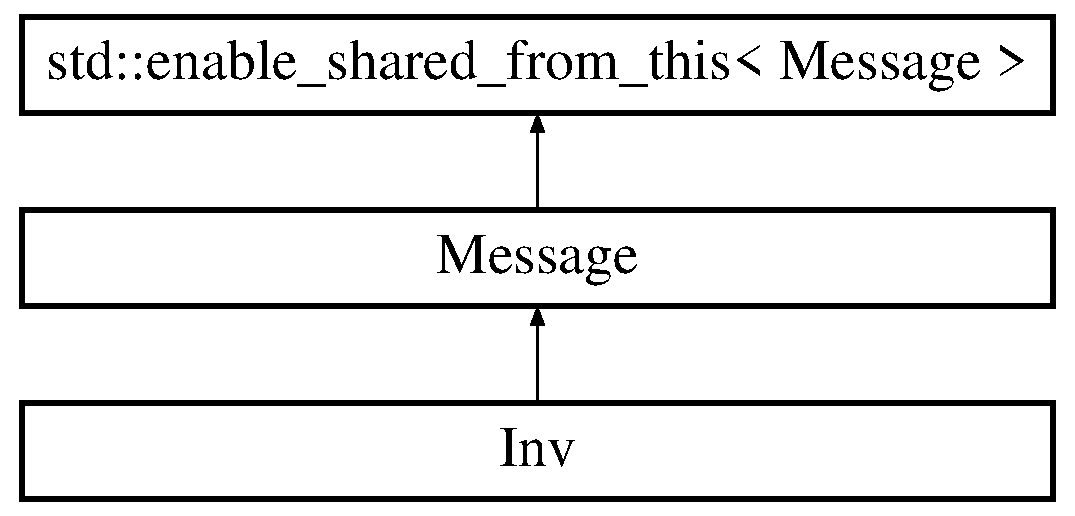
\includegraphics[height=3.000000cm]{classInv}
\end{center}
\end{figure}
\subsection*{Public Member Functions}
\begin{DoxyCompactItemize}
\item 
\mbox{\hyperlink{classInv_adb19ce28d1bf632581bfe7f7c3a3e9e1}{Inv}} (\mbox{\hyperlink{structInvData}{Inv\+Data}} dt)
\item 
\mbox{\hyperlink{classInv_a4b26ec79d84c931c4e09d0c1111c4f74}{Inv}} (rapidjson\+::\+Document $\ast$doc)
\item 
rapidjson\+::\+Value \mbox{\hyperlink{classInv_a815854f9808009dbf9f0fdb1159061c5}{json}} (rapidjson\+::\+Document $\ast$document) const override
\end{DoxyCompactItemize}
\subsection*{Private Attributes}
\begin{DoxyCompactItemize}
\item 
\mbox{\hyperlink{structInvData}{Inv\+Data}} \mbox{\hyperlink{classInv_a6d4e11f9a1b4ff85c7afc65fc21bc4a9}{data}}
\end{DoxyCompactItemize}
\subsection*{Additional Inherited Members}


\subsection{Constructor \& Destructor Documentation}
\mbox{\Hypertarget{classInv_adb19ce28d1bf632581bfe7f7c3a3e9e1}\label{classInv_adb19ce28d1bf632581bfe7f7c3a3e9e1}} 
\index{Inv@{Inv}!Inv@{Inv}}
\index{Inv@{Inv}!Inv@{Inv}}
\subsubsection{\texorpdfstring{Inv()}{Inv()}\hspace{0.1cm}{\footnotesize\ttfamily [1/2]}}
{\footnotesize\ttfamily Inv\+::\+Inv (\begin{DoxyParamCaption}\item[{\mbox{\hyperlink{structInvData}{Inv\+Data}}}]{dt }\end{DoxyParamCaption})\hspace{0.3cm}{\ttfamily [explicit]}}

\mbox{\Hypertarget{classInv_a4b26ec79d84c931c4e09d0c1111c4f74}\label{classInv_a4b26ec79d84c931c4e09d0c1111c4f74}} 
\index{Inv@{Inv}!Inv@{Inv}}
\index{Inv@{Inv}!Inv@{Inv}}
\subsubsection{\texorpdfstring{Inv()}{Inv()}\hspace{0.1cm}{\footnotesize\ttfamily [2/2]}}
{\footnotesize\ttfamily Inv\+::\+Inv (\begin{DoxyParamCaption}\item[{rapidjson\+::\+Document $\ast$}]{doc }\end{DoxyParamCaption})\hspace{0.3cm}{\ttfamily [explicit]}}



\subsection{Member Function Documentation}
\mbox{\Hypertarget{classInv_a815854f9808009dbf9f0fdb1159061c5}\label{classInv_a815854f9808009dbf9f0fdb1159061c5}} 
\index{Inv@{Inv}!json@{json}}
\index{json@{json}!Inv@{Inv}}
\subsubsection{\texorpdfstring{json()}{json()}}
{\footnotesize\ttfamily rapidjson\+::\+Value Inv\+::json (\begin{DoxyParamCaption}\item[{rapidjson\+::\+Document $\ast$}]{document }\end{DoxyParamCaption}) const\hspace{0.3cm}{\ttfamily [override]}, {\ttfamily [virtual]}}



Reimplemented from \mbox{\hyperlink{classMessage_a6f8e3ac2eed3a8afe9400fcd5b3447b2}{Message}}.



\subsection{Member Data Documentation}
\mbox{\Hypertarget{classInv_a6d4e11f9a1b4ff85c7afc65fc21bc4a9}\label{classInv_a6d4e11f9a1b4ff85c7afc65fc21bc4a9}} 
\index{Inv@{Inv}!data@{data}}
\index{data@{data}!Inv@{Inv}}
\subsubsection{\texorpdfstring{data}{data}}
{\footnotesize\ttfamily \mbox{\hyperlink{structInvData}{Inv\+Data}} Inv\+::data\hspace{0.3cm}{\ttfamily [private]}}



The documentation for this class was generated from the following files\+:\begin{DoxyCompactItemize}
\item 
include/\mbox{\hyperlink{messages_8hpp}{messages.\+hpp}}\item 
src/message/\mbox{\hyperlink{inv_8cpp}{inv.\+cpp}}\end{DoxyCompactItemize}

\hypertarget{structInvData}{}\section{Inv\+Data Struct Reference}
\label{structInvData}\index{Inv\+Data@{Inv\+Data}}


{\ttfamily \#include $<$messages.\+hpp$>$}

\subsection*{Public Member Functions}
\begin{DoxyCompactItemize}
\item 
\mbox{\hyperlink{structInvData_a04e2f1104af7ef52d684101c61a4873b}{Inv\+Data}} (std\+::string t, std\+::vector$<$ std\+::string $>$ hL)
\item 
\mbox{\hyperlink{structInvData_af6b3a71e6b4e0487f33ccf0b22a38813}{Inv\+Data}} (rapidjson\+::\+Value $\ast$val)
\item 
rapidjson\+::\+Value \mbox{\hyperlink{structInvData_a660c6492448faa3a19ac27c62047152d}{json}} (rapidjson\+::\+Document $\ast$doc) const
\end{DoxyCompactItemize}
\subsection*{Public Attributes}
\begin{DoxyCompactItemize}
\item 
std\+::string \mbox{\hyperlink{structInvData_a65d4044e395865238407578784cfccea}{type}}
\item 
std\+::vector$<$ std\+::string $>$ \mbox{\hyperlink{structInvData_ac7cd0400472c8a41a86960bc37ad7a3d}{hashes}}
\end{DoxyCompactItemize}


\subsection{Constructor \& Destructor Documentation}
\mbox{\Hypertarget{structInvData_a04e2f1104af7ef52d684101c61a4873b}\label{structInvData_a04e2f1104af7ef52d684101c61a4873b}} 
\index{Inv\+Data@{Inv\+Data}!Inv\+Data@{Inv\+Data}}
\index{Inv\+Data@{Inv\+Data}!Inv\+Data@{Inv\+Data}}
\subsubsection{\texorpdfstring{Inv\+Data()}{InvData()}\hspace{0.1cm}{\footnotesize\ttfamily [1/2]}}
{\footnotesize\ttfamily Inv\+Data\+::\+Inv\+Data (\begin{DoxyParamCaption}\item[{std\+::string}]{t,  }\item[{std\+::vector$<$ std\+::string $>$}]{hL }\end{DoxyParamCaption})}

\mbox{\Hypertarget{structInvData_af6b3a71e6b4e0487f33ccf0b22a38813}\label{structInvData_af6b3a71e6b4e0487f33ccf0b22a38813}} 
\index{Inv\+Data@{Inv\+Data}!Inv\+Data@{Inv\+Data}}
\index{Inv\+Data@{Inv\+Data}!Inv\+Data@{Inv\+Data}}
\subsubsection{\texorpdfstring{Inv\+Data()}{InvData()}\hspace{0.1cm}{\footnotesize\ttfamily [2/2]}}
{\footnotesize\ttfamily Inv\+Data\+::\+Inv\+Data (\begin{DoxyParamCaption}\item[{rapidjson\+::\+Value $\ast$}]{val }\end{DoxyParamCaption})\hspace{0.3cm}{\ttfamily [explicit]}}



\subsection{Member Function Documentation}
\mbox{\Hypertarget{structInvData_a660c6492448faa3a19ac27c62047152d}\label{structInvData_a660c6492448faa3a19ac27c62047152d}} 
\index{Inv\+Data@{Inv\+Data}!json@{json}}
\index{json@{json}!Inv\+Data@{Inv\+Data}}
\subsubsection{\texorpdfstring{json()}{json()}}
{\footnotesize\ttfamily rapidjson\+::\+Value Inv\+Data\+::json (\begin{DoxyParamCaption}\item[{rapidjson\+::\+Document $\ast$}]{doc }\end{DoxyParamCaption}) const}



\subsection{Member Data Documentation}
\mbox{\Hypertarget{structInvData_ac7cd0400472c8a41a86960bc37ad7a3d}\label{structInvData_ac7cd0400472c8a41a86960bc37ad7a3d}} 
\index{Inv\+Data@{Inv\+Data}!hashes@{hashes}}
\index{hashes@{hashes}!Inv\+Data@{Inv\+Data}}
\subsubsection{\texorpdfstring{hashes}{hashes}}
{\footnotesize\ttfamily std\+::vector$<$std\+::string$>$ Inv\+Data\+::hashes}

\mbox{\Hypertarget{structInvData_a65d4044e395865238407578784cfccea}\label{structInvData_a65d4044e395865238407578784cfccea}} 
\index{Inv\+Data@{Inv\+Data}!type@{type}}
\index{type@{type}!Inv\+Data@{Inv\+Data}}
\subsubsection{\texorpdfstring{type}{type}}
{\footnotesize\ttfamily std\+::string Inv\+Data\+::type}



The documentation for this struct was generated from the following files\+:\begin{DoxyCompactItemize}
\item 
include/\mbox{\hyperlink{messages_8hpp}{messages.\+hpp}}\item 
src/message/\mbox{\hyperlink{inv_8cpp}{inv.\+cpp}}\end{DoxyCompactItemize}

\hypertarget{classMempool}{}\section{Mempool Class Reference}
\label{classMempool}\index{Mempool@{Mempool}}


Pool of \mbox{\hyperlink{classTransaction}{Transaction}} not in \mbox{\hyperlink{classBlock}{Block}}.  




{\ttfamily \#include $<$mempool.\+hpp$>$}

\subsection*{Public Member Functions}
\begin{DoxyCompactItemize}
\item 
\mbox{\hyperlink{classMempool_a7d26cf499215b7660b991b03f20937dd}{Mempool}} ()
\begin{DoxyCompactList}\small\item\em Construct \mbox{\hyperlink{classMempool}{Mempool}} and load Level\+DB. \end{DoxyCompactList}\item 
bool \mbox{\hyperlink{classMempool_a7f1fff7b367c389ed3c8b847dde46add}{add\+Transaction}} (std\+::shared\+\_\+ptr$<$ \mbox{\hyperlink{classTransaction}{Transaction}} $>$ tr)
\begin{DoxyCompactList}\small\item\em Add \mbox{\hyperlink{classTransaction}{Transaction}} to \mbox{\hyperlink{classMempool}{Mempool}}. \end{DoxyCompactList}\item 
int \mbox{\hyperlink{classMempool_ab2b01cf87f14318e182b56462c0bf4f6}{get\+Input\+Value}} (\mbox{\hyperlink{utxo_8hpp_a19091d002da03ec92277e19295ac4540}{U\+T\+XO}} id) const
\begin{DoxyCompactList}\small\item\em Get value of U\+T\+XO. \end{DoxyCompactList}\item 
bool \mbox{\hyperlink{classMempool_a3a11892f1519132f81204e57cc758666}{exists}} (std\+::string tx\+Hash) const
\begin{DoxyCompactList}\small\item\em Checks if \mbox{\hyperlink{classTransaction}{Transaction}} exists in \mbox{\hyperlink{classMempool}{Mempool}}. \end{DoxyCompactList}\item 
bool \mbox{\hyperlink{classMempool_aef85ab57fba69a29f857d805a54a5358}{orphan\+Exists}} (std\+::string tx\+Hash) const
\begin{DoxyCompactList}\small\item\em Check if a \mbox{\hyperlink{classTransaction}{Transaction}} is a registered Orphan. \end{DoxyCompactList}\item 
bool \mbox{\hyperlink{classMempool_ad72ddf2809bf532f2b6c0f09922a77db}{output\+Exists}} (\mbox{\hyperlink{utxo_8hpp_a19091d002da03ec92277e19295ac4540}{U\+T\+XO}} id) const
\begin{DoxyCompactList}\small\item\em Check if a indexed output exists. \end{DoxyCompactList}\item 
bool \mbox{\hyperlink{classMempool_a6ccb56de239266bd5cebafac3112b31e}{is\+Orphan}} (std\+::shared\+\_\+ptr$<$ \mbox{\hyperlink{classTransaction}{Transaction}} $>$ tx) const
\begin{DoxyCompactList}\small\item\em Check if a \mbox{\hyperlink{classTransaction}{Transaction}} is Orphan. \end{DoxyCompactList}\item 
std\+::string \mbox{\hyperlink{classMempool_a93dc7c390ae5b561219cd654beddc36a}{get\+Hash\+Signature}} (\mbox{\hyperlink{utxo_8hpp_a19091d002da03ec92277e19295ac4540}{U\+T\+XO}} id) const
\begin{DoxyCompactList}\small\item\em Gets the hash used to sign a \mbox{\hyperlink{classTransaction}{Transaction}}. \end{DoxyCompactList}\item 
bool \mbox{\hyperlink{classMempool_a6ac1288e72c47a9c63841696901d7f3c}{is\+Spendable}} (\mbox{\hyperlink{utxo_8hpp_a19091d002da03ec92277e19295ac4540}{U\+T\+XO}} id) const
\begin{DoxyCompactList}\small\item\em Check if an output can be spent. \end{DoxyCompactList}\item 
std\+::vector$<$ std\+::string $>$ \mbox{\hyperlink{classMempool_ae76e6aba14cedd96990b40d08c47ad1d}{get\+Output\+Script}} (\mbox{\hyperlink{utxo_8hpp_a19091d002da03ec92277e19295ac4540}{U\+T\+XO}} id) const
\begin{DoxyCompactList}\small\item\em Get the script of an output. \end{DoxyCompactList}\item 
void \mbox{\hyperlink{classMempool_ad6bb7b0310265f592a29ff9a06656333}{increment\+Height}} ()
\begin{DoxyCompactList}\small\item\em Add one to the current\+Height. \end{DoxyCompactList}\item 
void \mbox{\hyperlink{classMempool_a6306559877a38806f0a3a90aa87f8655}{decrement\+Height}} ()
\begin{DoxyCompactList}\small\item\em Remove one from the current\+Height. \end{DoxyCompactList}\item 
std\+::vector$<$ \mbox{\hyperlink{utxo_8hpp_a19091d002da03ec92277e19295ac4540}{U\+T\+XO}} $>$ \mbox{\hyperlink{classMempool_a54749b3d653ebd1db396fefb1bfc137c}{orphan\+Deps}} (std\+::shared\+\_\+ptr$<$ \mbox{\hyperlink{classTransaction}{Transaction}} $>$ tx) const
\begin{DoxyCompactList}\small\item\em Get all inputs which are Orphan. \end{DoxyCompactList}\item 
\mbox{\hyperlink{transaction_8hpp_a379269e60c4ed3fb09a01778f31ddaad}{T\+X\+Type}} \mbox{\hyperlink{classMempool_a216beee85149f61c603ef8ad5cdd8ef5}{type}} (std\+::string tx\+Hash) const
\begin{DoxyCompactList}\small\item\em Gets the type of a registered \mbox{\hyperlink{classTransaction}{Transaction}}. \end{DoxyCompactList}\end{DoxyCompactItemize}
\subsection*{Private Member Functions}
\begin{DoxyCompactItemize}
\item 
void \mbox{\hyperlink{classMempool_ae658e1104b650fbc63786bc5e77fb328}{update\+Orphan}} (std\+::string orphan\+Hash)
\begin{DoxyCompactList}\small\item\em Handle an output being registered. \end{DoxyCompactList}\item 
bool \mbox{\hyperlink{classMempool_a589b0f1f4f88862bab6627771574e297}{check\+Orphan}} (std\+::string orphan\+Hash) const
\begin{DoxyCompactList}\small\item\em Checks if an orphan is still orphan. \end{DoxyCompactList}\end{DoxyCompactItemize}
\subsection*{Private Attributes}
\begin{DoxyCompactItemize}
\item 
\mbox{\hyperlink{classUTXOManager}{U\+T\+X\+O\+Manager}} \mbox{\hyperlink{classMempool_a84442d6065be70b7411d4376887c7858}{utxos}}
\item 
int \mbox{\hyperlink{classMempool_ad4ec0d1398ded82c7324a099b92b80cc}{current\+Height}}
\begin{DoxyCompactList}\small\item\em Height of the \mbox{\hyperlink{classBlockchain}{Blockchain}}. \end{DoxyCompactList}\item 
\mbox{\hyperlink{classHashMemory}{Hash\+Memory}}$<$ \mbox{\hyperlink{classTransaction}{Transaction}} $>$ \mbox{\hyperlink{classMempool_a6c0f587b34c99369786379717b0b1347}{main\+Pool}}
\item 
\mbox{\hyperlink{classHashMemory}{Hash\+Memory}}$<$ \mbox{\hyperlink{classTransaction}{Transaction}} $>$ \mbox{\hyperlink{classMempool_a215dd76ed87ac826511573e8fc91885a}{orphans}}
\item 
std\+::map$<$ std\+::string, std\+::string $>$ \mbox{\hyperlink{classMempool_a6a590208186b95856029bfa2613fbf04}{orphan\+Using\+U\+T\+XO}}
\begin{DoxyCompactList}\small\item\em Map of orphan using an U\+T\+XO. \end{DoxyCompactList}\end{DoxyCompactItemize}


\subsection{Detailed Description}
Pool of \mbox{\hyperlink{classTransaction}{Transaction}} not in \mbox{\hyperlink{classBlock}{Block}}. 

\subsection{Constructor \& Destructor Documentation}
\mbox{\Hypertarget{classMempool_a7d26cf499215b7660b991b03f20937dd}\label{classMempool_a7d26cf499215b7660b991b03f20937dd}} 
\index{Mempool@{Mempool}!Mempool@{Mempool}}
\index{Mempool@{Mempool}!Mempool@{Mempool}}
\subsubsection{\texorpdfstring{Mempool()}{Mempool()}}
{\footnotesize\ttfamily Mempool\+::\+Mempool (\begin{DoxyParamCaption}{ }\end{DoxyParamCaption})}



Construct \mbox{\hyperlink{classMempool}{Mempool}} and load Level\+DB. 



\subsection{Member Function Documentation}
\mbox{\Hypertarget{classMempool_a7f1fff7b367c389ed3c8b847dde46add}\label{classMempool_a7f1fff7b367c389ed3c8b847dde46add}} 
\index{Mempool@{Mempool}!add\+Transaction@{add\+Transaction}}
\index{add\+Transaction@{add\+Transaction}!Mempool@{Mempool}}
\subsubsection{\texorpdfstring{add\+Transaction()}{addTransaction()}}
{\footnotesize\ttfamily bool Mempool\+::add\+Transaction (\begin{DoxyParamCaption}\item[{std\+::shared\+\_\+ptr$<$ \mbox{\hyperlink{classTransaction}{Transaction}} $>$}]{tr }\end{DoxyParamCaption})}



Add \mbox{\hyperlink{classTransaction}{Transaction}} to \mbox{\hyperlink{classMempool}{Mempool}}. 


\begin{DoxyParams}{Parameters}
{\em tr} & \mbox{\hyperlink{classTransaction}{Transaction}} to add\\
\hline
\end{DoxyParams}
Checks if \mbox{\hyperlink{classTransaction}{Transaction}} is Orphan and is it is valid \mbox{\Hypertarget{classMempool_a589b0f1f4f88862bab6627771574e297}\label{classMempool_a589b0f1f4f88862bab6627771574e297}} 
\index{Mempool@{Mempool}!check\+Orphan@{check\+Orphan}}
\index{check\+Orphan@{check\+Orphan}!Mempool@{Mempool}}
\subsubsection{\texorpdfstring{check\+Orphan()}{checkOrphan()}}
{\footnotesize\ttfamily bool Mempool\+::check\+Orphan (\begin{DoxyParamCaption}\item[{std\+::string}]{orphan\+Hash }\end{DoxyParamCaption}) const\hspace{0.3cm}{\ttfamily [private]}}



Checks if an orphan is still orphan. 


\begin{DoxyParams}{Parameters}
{\em orphan\+Hash} & ash of an Orphan \mbox{\hyperlink{classTransaction}{Transaction}} \\
\hline
\end{DoxyParams}
\mbox{\Hypertarget{classMempool_a6306559877a38806f0a3a90aa87f8655}\label{classMempool_a6306559877a38806f0a3a90aa87f8655}} 
\index{Mempool@{Mempool}!decrement\+Height@{decrement\+Height}}
\index{decrement\+Height@{decrement\+Height}!Mempool@{Mempool}}
\subsubsection{\texorpdfstring{decrement\+Height()}{decrementHeight()}}
{\footnotesize\ttfamily void Mempool\+::decrement\+Height (\begin{DoxyParamCaption}{ }\end{DoxyParamCaption})}



Remove one from the current\+Height. 

\mbox{\Hypertarget{classMempool_a3a11892f1519132f81204e57cc758666}\label{classMempool_a3a11892f1519132f81204e57cc758666}} 
\index{Mempool@{Mempool}!exists@{exists}}
\index{exists@{exists}!Mempool@{Mempool}}
\subsubsection{\texorpdfstring{exists()}{exists()}}
{\footnotesize\ttfamily bool Mempool\+::exists (\begin{DoxyParamCaption}\item[{std\+::string}]{tx\+Hash }\end{DoxyParamCaption}) const}



Checks if \mbox{\hyperlink{classTransaction}{Transaction}} exists in \mbox{\hyperlink{classMempool}{Mempool}}. 


\begin{DoxyParams}{Parameters}
{\em tx\+Hash} & hash of a \mbox{\hyperlink{classTransaction}{Transaction}} \\
\hline
\end{DoxyParams}
\mbox{\Hypertarget{classMempool_a93dc7c390ae5b561219cd654beddc36a}\label{classMempool_a93dc7c390ae5b561219cd654beddc36a}} 
\index{Mempool@{Mempool}!get\+Hash\+Signature@{get\+Hash\+Signature}}
\index{get\+Hash\+Signature@{get\+Hash\+Signature}!Mempool@{Mempool}}
\subsubsection{\texorpdfstring{get\+Hash\+Signature()}{getHashSignature()}}
{\footnotesize\ttfamily std\+::string Mempool\+::get\+Hash\+Signature (\begin{DoxyParamCaption}\item[{\mbox{\hyperlink{utxo_8hpp_a19091d002da03ec92277e19295ac4540}{U\+T\+XO}}}]{id }\end{DoxyParamCaption}) const}



Gets the hash used to sign a \mbox{\hyperlink{classTransaction}{Transaction}}. 


\begin{DoxyParams}{Parameters}
{\em id} & reference to the \mbox{\hyperlink{classTransaction}{Transaction}} \\
\hline
\end{DoxyParams}
\mbox{\Hypertarget{classMempool_ab2b01cf87f14318e182b56462c0bf4f6}\label{classMempool_ab2b01cf87f14318e182b56462c0bf4f6}} 
\index{Mempool@{Mempool}!get\+Input\+Value@{get\+Input\+Value}}
\index{get\+Input\+Value@{get\+Input\+Value}!Mempool@{Mempool}}
\subsubsection{\texorpdfstring{get\+Input\+Value()}{getInputValue()}}
{\footnotesize\ttfamily int Mempool\+::get\+Input\+Value (\begin{DoxyParamCaption}\item[{\mbox{\hyperlink{utxo_8hpp_a19091d002da03ec92277e19295ac4540}{U\+T\+XO}}}]{id }\end{DoxyParamCaption}) const}



Get value of U\+T\+XO. 


\begin{DoxyParams}{Parameters}
{\em id} & reference to a \mbox{\hyperlink{classTransaction}{Transaction}} \\
\hline
\end{DoxyParams}
\begin{DoxyReturn}{Returns}
Gets the value of the output pointed by the U\+T\+XO 
\end{DoxyReturn}
\mbox{\Hypertarget{classMempool_ae76e6aba14cedd96990b40d08c47ad1d}\label{classMempool_ae76e6aba14cedd96990b40d08c47ad1d}} 
\index{Mempool@{Mempool}!get\+Output\+Script@{get\+Output\+Script}}
\index{get\+Output\+Script@{get\+Output\+Script}!Mempool@{Mempool}}
\subsubsection{\texorpdfstring{get\+Output\+Script()}{getOutputScript()}}
{\footnotesize\ttfamily std\+::vector$<$ std\+::string $>$ Mempool\+::get\+Output\+Script (\begin{DoxyParamCaption}\item[{\mbox{\hyperlink{utxo_8hpp_a19091d002da03ec92277e19295ac4540}{U\+T\+XO}}}]{id }\end{DoxyParamCaption}) const}



Get the script of an output. 


\begin{DoxyParams}{Parameters}
{\em id} & Transation\+Output to get the script from \\
\hline
\end{DoxyParams}
\mbox{\Hypertarget{classMempool_ad6bb7b0310265f592a29ff9a06656333}\label{classMempool_ad6bb7b0310265f592a29ff9a06656333}} 
\index{Mempool@{Mempool}!increment\+Height@{increment\+Height}}
\index{increment\+Height@{increment\+Height}!Mempool@{Mempool}}
\subsubsection{\texorpdfstring{increment\+Height()}{incrementHeight()}}
{\footnotesize\ttfamily void Mempool\+::increment\+Height (\begin{DoxyParamCaption}{ }\end{DoxyParamCaption})}



Add one to the current\+Height. 

\mbox{\Hypertarget{classMempool_a6ccb56de239266bd5cebafac3112b31e}\label{classMempool_a6ccb56de239266bd5cebafac3112b31e}} 
\index{Mempool@{Mempool}!is\+Orphan@{is\+Orphan}}
\index{is\+Orphan@{is\+Orphan}!Mempool@{Mempool}}
\subsubsection{\texorpdfstring{is\+Orphan()}{isOrphan()}}
{\footnotesize\ttfamily bool Mempool\+::is\+Orphan (\begin{DoxyParamCaption}\item[{std\+::shared\+\_\+ptr$<$ \mbox{\hyperlink{classTransaction}{Transaction}} $>$}]{tx }\end{DoxyParamCaption}) const}



Check if a \mbox{\hyperlink{classTransaction}{Transaction}} is Orphan. 


\begin{DoxyParams}{Parameters}
{\em tx} & \mbox{\hyperlink{classTransaction}{Transaction}} to identify \\
\hline
\end{DoxyParams}
\mbox{\Hypertarget{classMempool_a6ac1288e72c47a9c63841696901d7f3c}\label{classMempool_a6ac1288e72c47a9c63841696901d7f3c}} 
\index{Mempool@{Mempool}!is\+Spendable@{is\+Spendable}}
\index{is\+Spendable@{is\+Spendable}!Mempool@{Mempool}}
\subsubsection{\texorpdfstring{is\+Spendable()}{isSpendable()}}
{\footnotesize\ttfamily bool Mempool\+::is\+Spendable (\begin{DoxyParamCaption}\item[{\mbox{\hyperlink{utxo_8hpp_a19091d002da03ec92277e19295ac4540}{U\+T\+XO}}}]{id }\end{DoxyParamCaption}) const}



Check if an output can be spent. 


\begin{DoxyParams}{Parameters}
{\em id} & reference to an output \\
\hline
\end{DoxyParams}
\begin{DoxyReturn}{Returns}
True if the \mbox{\hyperlink{classTransaction}{Transaction}} is regular or if it is a coinbase and 42 \mbox{\hyperlink{classBlock}{Block}} have passed 
\end{DoxyReturn}
\mbox{\Hypertarget{classMempool_a54749b3d653ebd1db396fefb1bfc137c}\label{classMempool_a54749b3d653ebd1db396fefb1bfc137c}} 
\index{Mempool@{Mempool}!orphan\+Deps@{orphan\+Deps}}
\index{orphan\+Deps@{orphan\+Deps}!Mempool@{Mempool}}
\subsubsection{\texorpdfstring{orphan\+Deps()}{orphanDeps()}}
{\footnotesize\ttfamily std\+::vector$<$ \mbox{\hyperlink{utxo_8hpp_a19091d002da03ec92277e19295ac4540}{U\+T\+XO}} $>$ Mempool\+::orphan\+Deps (\begin{DoxyParamCaption}\item[{std\+::shared\+\_\+ptr$<$ \mbox{\hyperlink{classTransaction}{Transaction}} $>$}]{tx }\end{DoxyParamCaption}) const}



Get all inputs which are Orphan. 


\begin{DoxyParams}{Parameters}
{\em tx} & \mbox{\hyperlink{classTransaction}{Transaction}} to check \\
\hline
\end{DoxyParams}
\mbox{\Hypertarget{classMempool_aef85ab57fba69a29f857d805a54a5358}\label{classMempool_aef85ab57fba69a29f857d805a54a5358}} 
\index{Mempool@{Mempool}!orphan\+Exists@{orphan\+Exists}}
\index{orphan\+Exists@{orphan\+Exists}!Mempool@{Mempool}}
\subsubsection{\texorpdfstring{orphan\+Exists()}{orphanExists()}}
{\footnotesize\ttfamily bool Mempool\+::orphan\+Exists (\begin{DoxyParamCaption}\item[{std\+::string}]{tx\+Hash }\end{DoxyParamCaption}) const}



Check if a \mbox{\hyperlink{classTransaction}{Transaction}} is a registered Orphan. 


\begin{DoxyParams}{Parameters}
{\em tx\+Hash} & hash of a \mbox{\hyperlink{classTransaction}{Transaction}} \\
\hline
\end{DoxyParams}
\mbox{\Hypertarget{classMempool_ad72ddf2809bf532f2b6c0f09922a77db}\label{classMempool_ad72ddf2809bf532f2b6c0f09922a77db}} 
\index{Mempool@{Mempool}!output\+Exists@{output\+Exists}}
\index{output\+Exists@{output\+Exists}!Mempool@{Mempool}}
\subsubsection{\texorpdfstring{output\+Exists()}{outputExists()}}
{\footnotesize\ttfamily bool Mempool\+::output\+Exists (\begin{DoxyParamCaption}\item[{\mbox{\hyperlink{utxo_8hpp_a19091d002da03ec92277e19295ac4540}{U\+T\+XO}}}]{id }\end{DoxyParamCaption}) const}



Check if a indexed output exists. 


\begin{DoxyParams}{Parameters}
{\em id} & hash and index of output \\
\hline
\end{DoxyParams}
\begin{DoxyReturn}{Returns}
True if and only in \mbox{\hyperlink{classTransaction}{Transaction}} exists in main\+Pool and has an input id.\+index 
\end{DoxyReturn}
\mbox{\Hypertarget{classMempool_a216beee85149f61c603ef8ad5cdd8ef5}\label{classMempool_a216beee85149f61c603ef8ad5cdd8ef5}} 
\index{Mempool@{Mempool}!type@{type}}
\index{type@{type}!Mempool@{Mempool}}
\subsubsection{\texorpdfstring{type()}{type()}}
{\footnotesize\ttfamily \mbox{\hyperlink{transaction_8hpp_a379269e60c4ed3fb09a01778f31ddaad}{T\+X\+Type}} Mempool\+::type (\begin{DoxyParamCaption}\item[{std\+::string}]{tx\+Hash }\end{DoxyParamCaption}) const}



Gets the type of a registered \mbox{\hyperlink{classTransaction}{Transaction}}. 


\begin{DoxyParams}{Parameters}
{\em tx\+Hash} & hash of the \mbox{\hyperlink{classTransaction}{Transaction}} \\
\hline
\end{DoxyParams}
\mbox{\Hypertarget{classMempool_ae658e1104b650fbc63786bc5e77fb328}\label{classMempool_ae658e1104b650fbc63786bc5e77fb328}} 
\index{Mempool@{Mempool}!update\+Orphan@{update\+Orphan}}
\index{update\+Orphan@{update\+Orphan}!Mempool@{Mempool}}
\subsubsection{\texorpdfstring{update\+Orphan()}{updateOrphan()}}
{\footnotesize\ttfamily void Mempool\+::update\+Orphan (\begin{DoxyParamCaption}\item[{std\+::string}]{orphan\+Hash }\end{DoxyParamCaption})\hspace{0.3cm}{\ttfamily [private]}}



Handle an output being registered. 


\begin{DoxyParams}{Parameters}
{\em orphan\+Hash} & update the orphan depending on a \mbox{\hyperlink{classTransaction}{Transaction}} \\
\hline
\end{DoxyParams}


\subsection{Member Data Documentation}
\mbox{\Hypertarget{classMempool_ad4ec0d1398ded82c7324a099b92b80cc}\label{classMempool_ad4ec0d1398ded82c7324a099b92b80cc}} 
\index{Mempool@{Mempool}!current\+Height@{current\+Height}}
\index{current\+Height@{current\+Height}!Mempool@{Mempool}}
\subsubsection{\texorpdfstring{current\+Height}{currentHeight}}
{\footnotesize\ttfamily int Mempool\+::current\+Height\hspace{0.3cm}{\ttfamily [private]}}



Height of the \mbox{\hyperlink{classBlockchain}{Blockchain}}. 

\mbox{\Hypertarget{classMempool_a6c0f587b34c99369786379717b0b1347}\label{classMempool_a6c0f587b34c99369786379717b0b1347}} 
\index{Mempool@{Mempool}!main\+Pool@{main\+Pool}}
\index{main\+Pool@{main\+Pool}!Mempool@{Mempool}}
\subsubsection{\texorpdfstring{main\+Pool}{mainPool}}
{\footnotesize\ttfamily \mbox{\hyperlink{classHashMemory}{Hash\+Memory}}$<$\mbox{\hyperlink{classTransaction}{Transaction}}$>$ Mempool\+::main\+Pool\hspace{0.3cm}{\ttfamily [private]}}

\mbox{\Hypertarget{classMempool_a215dd76ed87ac826511573e8fc91885a}\label{classMempool_a215dd76ed87ac826511573e8fc91885a}} 
\index{Mempool@{Mempool}!orphans@{orphans}}
\index{orphans@{orphans}!Mempool@{Mempool}}
\subsubsection{\texorpdfstring{orphans}{orphans}}
{\footnotesize\ttfamily \mbox{\hyperlink{classHashMemory}{Hash\+Memory}}$<$\mbox{\hyperlink{classTransaction}{Transaction}}$>$ Mempool\+::orphans\hspace{0.3cm}{\ttfamily [private]}}

\mbox{\Hypertarget{classMempool_a6a590208186b95856029bfa2613fbf04}\label{classMempool_a6a590208186b95856029bfa2613fbf04}} 
\index{Mempool@{Mempool}!orphan\+Using\+U\+T\+XO@{orphan\+Using\+U\+T\+XO}}
\index{orphan\+Using\+U\+T\+XO@{orphan\+Using\+U\+T\+XO}!Mempool@{Mempool}}
\subsubsection{\texorpdfstring{orphan\+Using\+U\+T\+XO}{orphanUsingUTXO}}
{\footnotesize\ttfamily std\+::map$<$ std\+::string , std\+::string $>$ Mempool\+::orphan\+Using\+U\+T\+XO\hspace{0.3cm}{\ttfamily [private]}}



Map of orphan using an U\+T\+XO. 

There by design can\textquotesingle{}t be more than one \mbox{\hyperlink{classTransaction}{Transaction}} using a specified output and as such you can reject all orphans refereing to the same input \mbox{\Hypertarget{classMempool_a84442d6065be70b7411d4376887c7858}\label{classMempool_a84442d6065be70b7411d4376887c7858}} 
\index{Mempool@{Mempool}!utxos@{utxos}}
\index{utxos@{utxos}!Mempool@{Mempool}}
\subsubsection{\texorpdfstring{utxos}{utxos}}
{\footnotesize\ttfamily \mbox{\hyperlink{classUTXOManager}{U\+T\+X\+O\+Manager}} Mempool\+::utxos\hspace{0.3cm}{\ttfamily [private]}}



The documentation for this class was generated from the following files\+:\begin{DoxyCompactItemize}
\item 
include/\mbox{\hyperlink{mempool_8hpp}{mempool.\+hpp}}\item 
src/\mbox{\hyperlink{mempool_8cpp}{mempool.\+cpp}}\end{DoxyCompactItemize}

\hypertarget{classMessage}{}\section{Message Class Reference}
\label{classMessage}\index{Message@{Message}}


{\ttfamily \#include $<$messages.\+hpp$>$}

Inheritance diagram for Message\+:\begin{figure}[H]
\begin{center}
\leavevmode
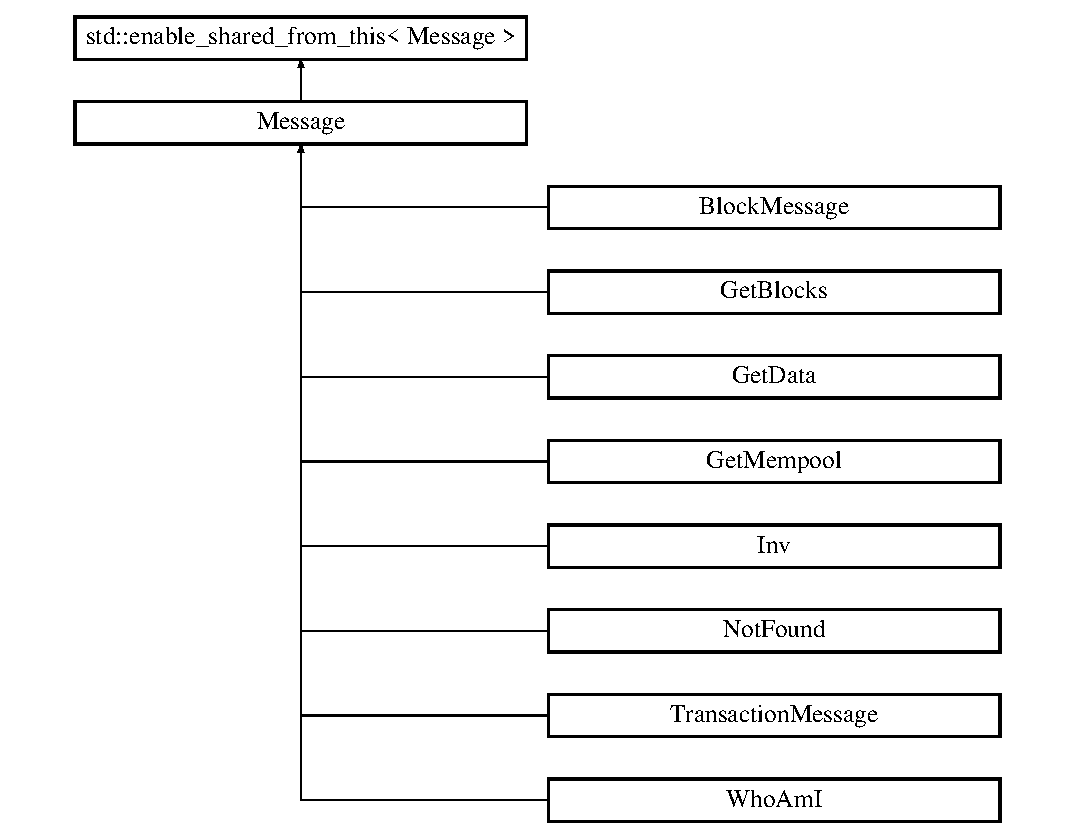
\includegraphics[height=10.000000cm]{classMessage}
\end{center}
\end{figure}
\subsection*{Public Types}
\begin{DoxyCompactItemize}
\item 
using \mbox{\hyperlink{classMessage_a3f7f2aa1058cb5f0b74a1fbb7fcd00e5}{message\+Pointer}} = std\+::shared\+\_\+ptr$<$ \mbox{\hyperlink{classMessage}{Message}} $>$
\end{DoxyCompactItemize}
\subsection*{Public Member Functions}
\begin{DoxyCompactItemize}
\item 
std\+::string \mbox{\hyperlink{classMessage_afde1ad2efd7e7af3ed65bbbb08e2e172}{str}} () const
\item 
std\+::string \mbox{\hyperlink{classMessage_aeb65039d076cefaff79b21044a4d8d29}{get\+Type}} () const
\item 
virtual rapidjson\+::\+Value \mbox{\hyperlink{classMessage_a6f8e3ac2eed3a8afe9400fcd5b3447b2}{json}} (rapidjson\+::\+Document $\ast$document) const
\item 
virtual \mbox{\hyperlink{classMessage_ad7ecaab66dfea90ed7bf9a3147bcf129}{$\sim$\+Message}} ()=0
\end{DoxyCompactItemize}
\subsection*{Protected Member Functions}
\begin{DoxyCompactItemize}
\item 
\mbox{\hyperlink{classMessage_aa222cbc5bf7865d5464a841740f45c11}{Message}} (std\+::string \mbox{\hyperlink{classMessage_ae9dead264183a4243c120026e6259b6f}{type}})
\item 
\mbox{\hyperlink{classMessage_a92ef92d05b8d6ca2647aff6eeb61df70}{Message}} (rapidjson\+::\+Document $\ast$doc)
\end{DoxyCompactItemize}
\subsection*{Protected Attributes}
\begin{DoxyCompactItemize}
\item 
int \mbox{\hyperlink{classMessage_a5bb4366b0a888886fec19ca2b2903d00}{magic}}
\item 
std\+::string \mbox{\hyperlink{classMessage_ae9dead264183a4243c120026e6259b6f}{type}}
\item 
std\+::time\+\_\+t \mbox{\hyperlink{classMessage_a78b882ca696ae5b4387b829132ff21ab}{timestamp}}
\end{DoxyCompactItemize}


\subsection{Member Typedef Documentation}
\mbox{\Hypertarget{classMessage_a3f7f2aa1058cb5f0b74a1fbb7fcd00e5}\label{classMessage_a3f7f2aa1058cb5f0b74a1fbb7fcd00e5}} 
\index{Message@{Message}!message\+Pointer@{message\+Pointer}}
\index{message\+Pointer@{message\+Pointer}!Message@{Message}}
\subsubsection{\texorpdfstring{message\+Pointer}{messagePointer}}
{\footnotesize\ttfamily using \mbox{\hyperlink{classMessage_a3f7f2aa1058cb5f0b74a1fbb7fcd00e5}{Message\+::message\+Pointer}} =  std\+::shared\+\_\+ptr$<$\mbox{\hyperlink{classMessage}{Message}}$>$}



\subsection{Constructor \& Destructor Documentation}
\mbox{\Hypertarget{classMessage_aa222cbc5bf7865d5464a841740f45c11}\label{classMessage_aa222cbc5bf7865d5464a841740f45c11}} 
\index{Message@{Message}!Message@{Message}}
\index{Message@{Message}!Message@{Message}}
\subsubsection{\texorpdfstring{Message()}{Message()}\hspace{0.1cm}{\footnotesize\ttfamily [1/2]}}
{\footnotesize\ttfamily Message\+::\+Message (\begin{DoxyParamCaption}\item[{std\+::string}]{type }\end{DoxyParamCaption})\hspace{0.3cm}{\ttfamily [explicit]}, {\ttfamily [protected]}}

\mbox{\Hypertarget{classMessage_a92ef92d05b8d6ca2647aff6eeb61df70}\label{classMessage_a92ef92d05b8d6ca2647aff6eeb61df70}} 
\index{Message@{Message}!Message@{Message}}
\index{Message@{Message}!Message@{Message}}
\subsubsection{\texorpdfstring{Message()}{Message()}\hspace{0.1cm}{\footnotesize\ttfamily [2/2]}}
{\footnotesize\ttfamily Message\+::\+Message (\begin{DoxyParamCaption}\item[{rapidjson\+::\+Document $\ast$}]{doc }\end{DoxyParamCaption})\hspace{0.3cm}{\ttfamily [explicit]}, {\ttfamily [protected]}}

\mbox{\Hypertarget{classMessage_ad7ecaab66dfea90ed7bf9a3147bcf129}\label{classMessage_ad7ecaab66dfea90ed7bf9a3147bcf129}} 
\index{Message@{Message}!````~Message@{$\sim$\+Message}}
\index{````~Message@{$\sim$\+Message}!Message@{Message}}
\subsubsection{\texorpdfstring{$\sim$\+Message()}{~Message()}}
{\footnotesize\ttfamily Message\+::$\sim$\+Message (\begin{DoxyParamCaption}{ }\end{DoxyParamCaption})\hspace{0.3cm}{\ttfamily [pure virtual]}}



\subsection{Member Function Documentation}
\mbox{\Hypertarget{classMessage_aeb65039d076cefaff79b21044a4d8d29}\label{classMessage_aeb65039d076cefaff79b21044a4d8d29}} 
\index{Message@{Message}!get\+Type@{get\+Type}}
\index{get\+Type@{get\+Type}!Message@{Message}}
\subsubsection{\texorpdfstring{get\+Type()}{getType()}}
{\footnotesize\ttfamily std\+::string Message\+::get\+Type (\begin{DoxyParamCaption}{ }\end{DoxyParamCaption}) const}

\mbox{\Hypertarget{classMessage_a6f8e3ac2eed3a8afe9400fcd5b3447b2}\label{classMessage_a6f8e3ac2eed3a8afe9400fcd5b3447b2}} 
\index{Message@{Message}!json@{json}}
\index{json@{json}!Message@{Message}}
\subsubsection{\texorpdfstring{json()}{json()}}
{\footnotesize\ttfamily Value Message\+::json (\begin{DoxyParamCaption}\item[{rapidjson\+::\+Document $\ast$}]{document }\end{DoxyParamCaption}) const\hspace{0.3cm}{\ttfamily [virtual]}}



Reimplemented in \mbox{\hyperlink{classGetMempool_a3e6fb495c609ade4e8efd3d5668c28cf}{Get\+Mempool}}, \mbox{\hyperlink{classGetBlocks_a8b77916e999ba0a730e31b90b4733928}{Get\+Blocks}}, \mbox{\hyperlink{classTransactionMessage_af8675087bd26b6aa0c30a3e3141dda4e}{Transaction\+Message}}, \mbox{\hyperlink{classBlockMessage_afe33ddfdae83a25d98dd28541bc2fcfe}{Block\+Message}}, \mbox{\hyperlink{classNotFound_a67ee661e6a87c681d167da585c106240}{Not\+Found}}, \mbox{\hyperlink{classGetData_a2fb121264fc1c5821e769f4f2389c6ff}{Get\+Data}}, \mbox{\hyperlink{classInv_a815854f9808009dbf9f0fdb1159061c5}{Inv}}, and \mbox{\hyperlink{classWhoAmI_a998c4b21d6235a84f15bd994b76be59d}{Who\+AmI}}.

\mbox{\Hypertarget{classMessage_afde1ad2efd7e7af3ed65bbbb08e2e172}\label{classMessage_afde1ad2efd7e7af3ed65bbbb08e2e172}} 
\index{Message@{Message}!str@{str}}
\index{str@{str}!Message@{Message}}
\subsubsection{\texorpdfstring{str()}{str()}}
{\footnotesize\ttfamily std\+::string Message\+::str (\begin{DoxyParamCaption}{ }\end{DoxyParamCaption}) const}



\subsection{Member Data Documentation}
\mbox{\Hypertarget{classMessage_a5bb4366b0a888886fec19ca2b2903d00}\label{classMessage_a5bb4366b0a888886fec19ca2b2903d00}} 
\index{Message@{Message}!magic@{magic}}
\index{magic@{magic}!Message@{Message}}
\subsubsection{\texorpdfstring{magic}{magic}}
{\footnotesize\ttfamily int Message\+::magic\hspace{0.3cm}{\ttfamily [protected]}}

\mbox{\Hypertarget{classMessage_a78b882ca696ae5b4387b829132ff21ab}\label{classMessage_a78b882ca696ae5b4387b829132ff21ab}} 
\index{Message@{Message}!timestamp@{timestamp}}
\index{timestamp@{timestamp}!Message@{Message}}
\subsubsection{\texorpdfstring{timestamp}{timestamp}}
{\footnotesize\ttfamily std\+::time\+\_\+t Message\+::timestamp\hspace{0.3cm}{\ttfamily [protected]}}

\mbox{\Hypertarget{classMessage_ae9dead264183a4243c120026e6259b6f}\label{classMessage_ae9dead264183a4243c120026e6259b6f}} 
\index{Message@{Message}!type@{type}}
\index{type@{type}!Message@{Message}}
\subsubsection{\texorpdfstring{type}{type}}
{\footnotesize\ttfamily std\+::string Message\+::type\hspace{0.3cm}{\ttfamily [protected]}}



The documentation for this class was generated from the following files\+:\begin{DoxyCompactItemize}
\item 
include/\mbox{\hyperlink{messages_8hpp}{messages.\+hpp}}\item 
src/message/\mbox{\hyperlink{messages_8cpp}{messages.\+cpp}}\end{DoxyCompactItemize}

\hypertarget{classNode}{}\section{Node Class Reference}
\label{classNode}\index{Node@{Node}}


\mbox{\hyperlink{classNode}{Node}} handling messages and processing.  




{\ttfamily \#include $<$node.\+hpp$>$}

\subsection*{Public Member Functions}
\begin{DoxyCompactItemize}
\item 
\mbox{\hyperlink{classNode_a69479b3f2c9ca25cc6f178c30c8b7da8}{Node}} (asio\+::io\+\_\+context \&io\+\_\+context)
\begin{DoxyCompactList}\small\item\em Construct a \mbox{\hyperlink{classNode}{Node}}. \end{DoxyCompactList}\item 
void \mbox{\hyperlink{classNode_a89bb61a94d73680b692280d83e83d2f4}{run}} ()
\begin{DoxyCompactList}\small\item\em Main loop of \mbox{\hyperlink{classNode}{Node}}. \end{DoxyCompactList}\end{DoxyCompactItemize}
\subsection*{Private Member Functions}
\begin{DoxyCompactItemize}
\item 
void \mbox{\hyperlink{classNode_a7955793e35a52f192e7e5f82dd541092}{handle\+Accept}} (\mbox{\hyperlink{classConnection_a1bb6cd8924ff091e9b053e3368735c9c}{Connection\+::pointer}} new\+Connection)
\begin{DoxyCompactList}\small\item\em Handles a connection. \end{DoxyCompactList}\end{DoxyCompactItemize}
\subsection*{Private Attributes}
\begin{DoxyCompactItemize}
\item 
\mbox{\hyperlink{classMempool}{Mempool}} \mbox{\hyperlink{classNode_a2c3b3df5c2c8f4b7e95e1aa3dfd80e25}{mempool}}
\item 
\mbox{\hyperlink{classBlockchain}{Blockchain}} \mbox{\hyperlink{classNode_a631d922988b25901cb0e98a5274c2588}{blockchain}}
\item 
asio\+::ip\+::tcp\+::acceptor \mbox{\hyperlink{classNode_a3b0f7b49f99b1aad5ffeffb5b721b7a0}{acceptor}}
\item 
std\+::vector$<$ \mbox{\hyperlink{classConnection_a1bb6cd8924ff091e9b053e3368735c9c}{Connection\+::pointer}} $>$ \mbox{\hyperlink{classNode_ab9ba07b806d024e8461fae70bea349c0}{connections}}
\begin{DoxyCompactList}\small\item\em Vector of all current connections. \end{DoxyCompactList}\end{DoxyCompactItemize}


\subsection{Detailed Description}
\mbox{\hyperlink{classNode}{Node}} handling messages and processing. 

\subsection{Constructor \& Destructor Documentation}
\mbox{\Hypertarget{classNode_a69479b3f2c9ca25cc6f178c30c8b7da8}\label{classNode_a69479b3f2c9ca25cc6f178c30c8b7da8}} 
\index{Node@{Node}!Node@{Node}}
\index{Node@{Node}!Node@{Node}}
\subsubsection{\texorpdfstring{Node()}{Node()}}
{\footnotesize\ttfamily Node\+::\+Node (\begin{DoxyParamCaption}\item[{asio\+::io\+\_\+context \&}]{io\+\_\+context }\end{DoxyParamCaption})\hspace{0.3cm}{\ttfamily [explicit]}}



Construct a \mbox{\hyperlink{classNode}{Node}}. 


\begin{DoxyParams}{Parameters}
{\em io\+\_\+context} & an asio\+::io\+\_\+context\\
\hline
\end{DoxyParams}
Executes the startup routine and creates mempools 

\subsection{Member Function Documentation}
\mbox{\Hypertarget{classNode_a7955793e35a52f192e7e5f82dd541092}\label{classNode_a7955793e35a52f192e7e5f82dd541092}} 
\index{Node@{Node}!handle\+Accept@{handle\+Accept}}
\index{handle\+Accept@{handle\+Accept}!Node@{Node}}
\subsubsection{\texorpdfstring{handle\+Accept()}{handleAccept()}}
{\footnotesize\ttfamily void Node\+::handle\+Accept (\begin{DoxyParamCaption}\item[{\mbox{\hyperlink{classConnection_a1bb6cd8924ff091e9b053e3368735c9c}{Connection\+::pointer}}}]{new\+Connection }\end{DoxyParamCaption})\hspace{0.3cm}{\ttfamily [private]}}



Handles a connection. 


\begin{DoxyParams}{Parameters}
{\em new\+Connection} & a shared pointer to the connection \\
\hline
\end{DoxyParams}
\mbox{\Hypertarget{classNode_a89bb61a94d73680b692280d83e83d2f4}\label{classNode_a89bb61a94d73680b692280d83e83d2f4}} 
\index{Node@{Node}!run@{run}}
\index{run@{run}!Node@{Node}}
\subsubsection{\texorpdfstring{run()}{run()}}
{\footnotesize\ttfamily void Node\+::run (\begin{DoxyParamCaption}{ }\end{DoxyParamCaption})}



Main loop of \mbox{\hyperlink{classNode}{Node}}. 



\subsection{Member Data Documentation}
\mbox{\Hypertarget{classNode_a3b0f7b49f99b1aad5ffeffb5b721b7a0}\label{classNode_a3b0f7b49f99b1aad5ffeffb5b721b7a0}} 
\index{Node@{Node}!acceptor@{acceptor}}
\index{acceptor@{acceptor}!Node@{Node}}
\subsubsection{\texorpdfstring{acceptor}{acceptor}}
{\footnotesize\ttfamily asio\+::ip\+::tcp\+::acceptor Node\+::acceptor\hspace{0.3cm}{\ttfamily [private]}}

\mbox{\Hypertarget{classNode_a631d922988b25901cb0e98a5274c2588}\label{classNode_a631d922988b25901cb0e98a5274c2588}} 
\index{Node@{Node}!blockchain@{blockchain}}
\index{blockchain@{blockchain}!Node@{Node}}
\subsubsection{\texorpdfstring{blockchain}{blockchain}}
{\footnotesize\ttfamily \mbox{\hyperlink{classBlockchain}{Blockchain}} Node\+::blockchain\hspace{0.3cm}{\ttfamily [private]}}

\mbox{\Hypertarget{classNode_ab9ba07b806d024e8461fae70bea349c0}\label{classNode_ab9ba07b806d024e8461fae70bea349c0}} 
\index{Node@{Node}!connections@{connections}}
\index{connections@{connections}!Node@{Node}}
\subsubsection{\texorpdfstring{connections}{connections}}
{\footnotesize\ttfamily std\+::vector$<$\mbox{\hyperlink{classConnection_a1bb6cd8924ff091e9b053e3368735c9c}{Connection\+::pointer}}$>$ Node\+::connections\hspace{0.3cm}{\ttfamily [private]}}



Vector of all current connections. 

\mbox{\Hypertarget{classNode_a2c3b3df5c2c8f4b7e95e1aa3dfd80e25}\label{classNode_a2c3b3df5c2c8f4b7e95e1aa3dfd80e25}} 
\index{Node@{Node}!mempool@{mempool}}
\index{mempool@{mempool}!Node@{Node}}
\subsubsection{\texorpdfstring{mempool}{mempool}}
{\footnotesize\ttfamily \mbox{\hyperlink{classMempool}{Mempool}} Node\+::mempool\hspace{0.3cm}{\ttfamily [private]}}



The documentation for this class was generated from the following files\+:\begin{DoxyCompactItemize}
\item 
include/\mbox{\hyperlink{node_8hpp}{node.\+hpp}}\item 
src/\mbox{\hyperlink{node_8cpp}{node.\+cpp}}\end{DoxyCompactItemize}

\hypertarget{classNotFound}{}\section{Not\+Found Class Reference}
\label{classNotFound}\index{Not\+Found@{Not\+Found}}


{\ttfamily \#include $<$messages.\+hpp$>$}

Inheritance diagram for Not\+Found\+:\begin{figure}[H]
\begin{center}
\leavevmode
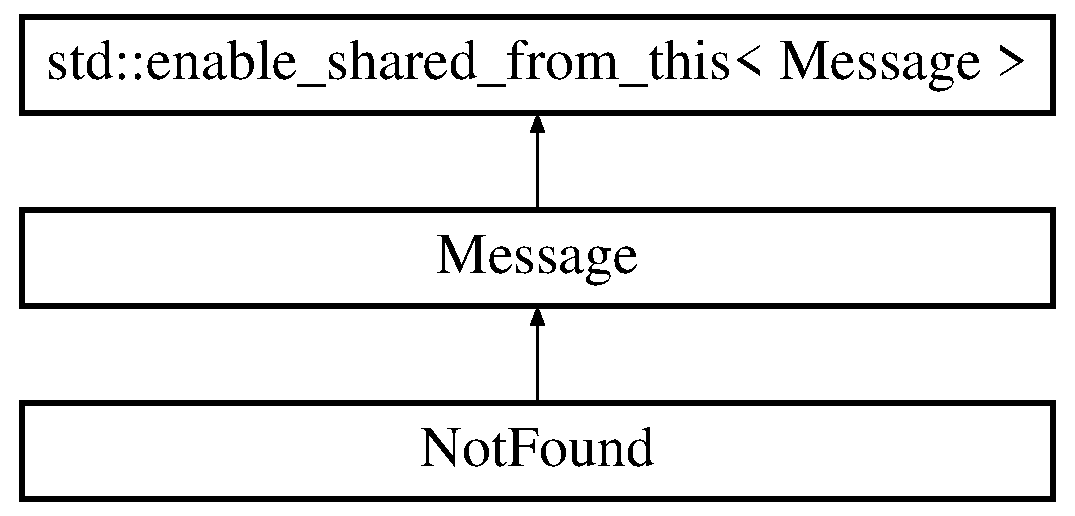
\includegraphics[height=3.000000cm]{classNotFound}
\end{center}
\end{figure}
\subsection*{Public Member Functions}
\begin{DoxyCompactItemize}
\item 
\mbox{\hyperlink{classNotFound_aa7fd834fc95565278a43553d7bae018c}{Not\+Found}} (std\+::string \mbox{\hyperlink{classNotFound_acd2ac9fcbc773b0acbe204fbc100316b}{res\+Type}}, std\+::string hash\+Type)
\item 
\mbox{\hyperlink{classNotFound_a52f321414fbd643f0af503f977f78078}{Not\+Found}} (rapidjson\+::\+Document $\ast$doc)
\item 
rapidjson\+::\+Value \mbox{\hyperlink{classNotFound_a67ee661e6a87c681d167da585c106240}{json}} (rapidjson\+::\+Document $\ast$document) const override
\end{DoxyCompactItemize}
\subsection*{Private Attributes}
\begin{DoxyCompactItemize}
\item 
std\+::string \mbox{\hyperlink{classNotFound_acd2ac9fcbc773b0acbe204fbc100316b}{res\+Type}}
\item 
std\+::string \mbox{\hyperlink{classNotFound_ace964753b12aac33c1f05bbdb6bf813b}{hash}}
\end{DoxyCompactItemize}
\subsection*{Additional Inherited Members}


\subsection{Constructor \& Destructor Documentation}
\mbox{\Hypertarget{classNotFound_aa7fd834fc95565278a43553d7bae018c}\label{classNotFound_aa7fd834fc95565278a43553d7bae018c}} 
\index{Not\+Found@{Not\+Found}!Not\+Found@{Not\+Found}}
\index{Not\+Found@{Not\+Found}!Not\+Found@{Not\+Found}}
\subsubsection{\texorpdfstring{Not\+Found()}{NotFound()}\hspace{0.1cm}{\footnotesize\ttfamily [1/2]}}
{\footnotesize\ttfamily Not\+Found\+::\+Not\+Found (\begin{DoxyParamCaption}\item[{std\+::string}]{res\+Type,  }\item[{std\+::string}]{hash\+Type }\end{DoxyParamCaption})}

\mbox{\Hypertarget{classNotFound_a52f321414fbd643f0af503f977f78078}\label{classNotFound_a52f321414fbd643f0af503f977f78078}} 
\index{Not\+Found@{Not\+Found}!Not\+Found@{Not\+Found}}
\index{Not\+Found@{Not\+Found}!Not\+Found@{Not\+Found}}
\subsubsection{\texorpdfstring{Not\+Found()}{NotFound()}\hspace{0.1cm}{\footnotesize\ttfamily [2/2]}}
{\footnotesize\ttfamily Not\+Found\+::\+Not\+Found (\begin{DoxyParamCaption}\item[{rapidjson\+::\+Document $\ast$}]{doc }\end{DoxyParamCaption})\hspace{0.3cm}{\ttfamily [explicit]}}



\subsection{Member Function Documentation}
\mbox{\Hypertarget{classNotFound_a67ee661e6a87c681d167da585c106240}\label{classNotFound_a67ee661e6a87c681d167da585c106240}} 
\index{Not\+Found@{Not\+Found}!json@{json}}
\index{json@{json}!Not\+Found@{Not\+Found}}
\subsubsection{\texorpdfstring{json()}{json()}}
{\footnotesize\ttfamily rapidjson\+::\+Value Not\+Found\+::json (\begin{DoxyParamCaption}\item[{rapidjson\+::\+Document $\ast$}]{document }\end{DoxyParamCaption}) const\hspace{0.3cm}{\ttfamily [override]}, {\ttfamily [virtual]}}



Reimplemented from \mbox{\hyperlink{classMessage_a6f8e3ac2eed3a8afe9400fcd5b3447b2}{Message}}.



\subsection{Member Data Documentation}
\mbox{\Hypertarget{classNotFound_ace964753b12aac33c1f05bbdb6bf813b}\label{classNotFound_ace964753b12aac33c1f05bbdb6bf813b}} 
\index{Not\+Found@{Not\+Found}!hash@{hash}}
\index{hash@{hash}!Not\+Found@{Not\+Found}}
\subsubsection{\texorpdfstring{hash}{hash}}
{\footnotesize\ttfamily std\+::string Not\+Found\+::hash\hspace{0.3cm}{\ttfamily [private]}}

\mbox{\Hypertarget{classNotFound_acd2ac9fcbc773b0acbe204fbc100316b}\label{classNotFound_acd2ac9fcbc773b0acbe204fbc100316b}} 
\index{Not\+Found@{Not\+Found}!res\+Type@{res\+Type}}
\index{res\+Type@{res\+Type}!Not\+Found@{Not\+Found}}
\subsubsection{\texorpdfstring{res\+Type}{resType}}
{\footnotesize\ttfamily std\+::string Not\+Found\+::res\+Type\hspace{0.3cm}{\ttfamily [private]}}



The documentation for this class was generated from the following files\+:\begin{DoxyCompactItemize}
\item 
include/\mbox{\hyperlink{messages_8hpp}{messages.\+hpp}}\item 
src/message/\mbox{\hyperlink{notfound_8cpp}{notfound.\+cpp}}\end{DoxyCompactItemize}

\hypertarget{structOutputTransaction}{}\section{Output\+Transaction Struct Reference}
\label{structOutputTransaction}\index{Output\+Transaction@{Output\+Transaction}}


{\ttfamily \#include $<$transaction.\+hpp$>$}

\subsection*{Public Member Functions}
\begin{DoxyCompactItemize}
\item 
std\+::string \mbox{\hyperlink{structOutputTransaction_a8491046e882593572512bf7717c36285}{str}} () const
\item 
Value \mbox{\hyperlink{structOutputTransaction_aa68e74419b5d85bcfa550ffbbe8a3287}{json}} (Document $\ast$document) const
\item 
void \mbox{\hyperlink{structOutputTransaction_a51ddd6b77522fa6fa676c00add6d6e1a}{load}} (Value $\ast$val)
\end{DoxyCompactItemize}
\subsection*{Public Attributes}
\begin{DoxyCompactItemize}
\item 
int \mbox{\hyperlink{structOutputTransaction_a938dbaea39f3d053581d744e21281ad4}{value}}
\item 
std\+::vector$<$ std\+::string $>$ \mbox{\hyperlink{structOutputTransaction_a32dcca6abe10eba274ba85f3460ceb84}{script\+Instructions}}
\end{DoxyCompactItemize}


\subsection{Member Function Documentation}
\mbox{\Hypertarget{structOutputTransaction_aa68e74419b5d85bcfa550ffbbe8a3287}\label{structOutputTransaction_aa68e74419b5d85bcfa550ffbbe8a3287}} 
\index{Output\+Transaction@{Output\+Transaction}!json@{json}}
\index{json@{json}!Output\+Transaction@{Output\+Transaction}}
\subsubsection{\texorpdfstring{json()}{json()}}
{\footnotesize\ttfamily Value Output\+Transaction\+::json (\begin{DoxyParamCaption}\item[{Document $\ast$}]{document }\end{DoxyParamCaption}) const}

\mbox{\Hypertarget{structOutputTransaction_a51ddd6b77522fa6fa676c00add6d6e1a}\label{structOutputTransaction_a51ddd6b77522fa6fa676c00add6d6e1a}} 
\index{Output\+Transaction@{Output\+Transaction}!load@{load}}
\index{load@{load}!Output\+Transaction@{Output\+Transaction}}
\subsubsection{\texorpdfstring{load()}{load()}}
{\footnotesize\ttfamily void Output\+Transaction\+::load (\begin{DoxyParamCaption}\item[{Value $\ast$}]{val }\end{DoxyParamCaption})}

\mbox{\Hypertarget{structOutputTransaction_a8491046e882593572512bf7717c36285}\label{structOutputTransaction_a8491046e882593572512bf7717c36285}} 
\index{Output\+Transaction@{Output\+Transaction}!str@{str}}
\index{str@{str}!Output\+Transaction@{Output\+Transaction}}
\subsubsection{\texorpdfstring{str()}{str()}}
{\footnotesize\ttfamily std\+::string Output\+Transaction\+::str (\begin{DoxyParamCaption}{ }\end{DoxyParamCaption}) const}



\subsection{Member Data Documentation}
\mbox{\Hypertarget{structOutputTransaction_a32dcca6abe10eba274ba85f3460ceb84}\label{structOutputTransaction_a32dcca6abe10eba274ba85f3460ceb84}} 
\index{Output\+Transaction@{Output\+Transaction}!script\+Instructions@{script\+Instructions}}
\index{script\+Instructions@{script\+Instructions}!Output\+Transaction@{Output\+Transaction}}
\subsubsection{\texorpdfstring{script\+Instructions}{scriptInstructions}}
{\footnotesize\ttfamily std\+::vector$<$std\+::string$>$ Output\+Transaction\+::script\+Instructions}

\mbox{\Hypertarget{structOutputTransaction_a938dbaea39f3d053581d744e21281ad4}\label{structOutputTransaction_a938dbaea39f3d053581d744e21281ad4}} 
\index{Output\+Transaction@{Output\+Transaction}!value@{value}}
\index{value@{value}!Output\+Transaction@{Output\+Transaction}}
\subsubsection{\texorpdfstring{value}{value}}
{\footnotesize\ttfamily int Output\+Transaction\+::value}



The documentation for this struct was generated from the following files\+:\begin{DoxyCompactItemize}
\item 
include/\mbox{\hyperlink{transaction_8hpp}{transaction.\+hpp}}\item 
src/transaction/\mbox{\hyperlink{transactionoutput_8cpp}{transactionoutput.\+cpp}}\end{DoxyCompactItemize}

\hypertarget{structHandler_1_1params}{}\section{Handler\+:\+:params Struct Reference}
\label{structHandler_1_1params}\index{Handler\+::params@{Handler\+::params}}
\subsection*{Public Attributes}
\begin{DoxyCompactItemize}
\item 
\mbox{\hyperlink{classMessage_a3f7f2aa1058cb5f0b74a1fbb7fcd00e5}{Message\+::message\+Pointer}} \mbox{\hyperlink{structHandler_1_1params_a2625bc9e0e823431c8039b587e0dd7ee}{message}}
\item 
\mbox{\hyperlink{classNode}{Node}} $\ast$ \mbox{\hyperlink{structHandler_1_1params_a9c2d75c37d122d3b8186a5b37c1d2526}{node}}
\item 
std\+::shared\+\_\+ptr$<$ \mbox{\hyperlink{classConnection}{Connection}} $>$ \mbox{\hyperlink{structHandler_1_1params_acea9549fb1dc08daadd963a1bcbd435e}{connection}}
\end{DoxyCompactItemize}


\subsection{Member Data Documentation}
\mbox{\Hypertarget{structHandler_1_1params_acea9549fb1dc08daadd963a1bcbd435e}\label{structHandler_1_1params_acea9549fb1dc08daadd963a1bcbd435e}} 
\index{Handler\+::params@{Handler\+::params}!connection@{connection}}
\index{connection@{connection}!Handler\+::params@{Handler\+::params}}
\subsubsection{\texorpdfstring{connection}{connection}}
{\footnotesize\ttfamily std\+::shared\+\_\+ptr$<$\mbox{\hyperlink{classConnection}{Connection}}$>$ Handler\+::params\+::connection}

\mbox{\Hypertarget{structHandler_1_1params_a2625bc9e0e823431c8039b587e0dd7ee}\label{structHandler_1_1params_a2625bc9e0e823431c8039b587e0dd7ee}} 
\index{Handler\+::params@{Handler\+::params}!message@{message}}
\index{message@{message}!Handler\+::params@{Handler\+::params}}
\subsubsection{\texorpdfstring{message}{message}}
{\footnotesize\ttfamily \mbox{\hyperlink{classMessage_a3f7f2aa1058cb5f0b74a1fbb7fcd00e5}{Message\+::message\+Pointer}} Handler\+::params\+::message}

\mbox{\Hypertarget{structHandler_1_1params_a9c2d75c37d122d3b8186a5b37c1d2526}\label{structHandler_1_1params_a9c2d75c37d122d3b8186a5b37c1d2526}} 
\index{Handler\+::params@{Handler\+::params}!node@{node}}
\index{node@{node}!Handler\+::params@{Handler\+::params}}
\subsubsection{\texorpdfstring{node}{node}}
{\footnotesize\ttfamily \mbox{\hyperlink{classNode}{Node}}$\ast$ Handler\+::params\+::node}



The documentation for this struct was generated from the following file\+:\begin{DoxyCompactItemize}
\item 
include/\mbox{\hyperlink{messagehandler_8hpp}{messagehandler.\+hpp}}\end{DoxyCompactItemize}

\hypertarget{classScript}{}\section{Script Class Reference}
\label{classScript}\index{Script@{Script}}


{\ttfamily \#include $<$script.\+hpp$>$}

\subsection*{Public Member Functions}
\begin{DoxyCompactItemize}
\item 
\mbox{\hyperlink{classScript_ac5dfef3a38ce09aa3d664b041b4b47e1}{Script}} (std\+::vector$<$ std\+::string $>$\+::iterator inital\+Instruction, std\+::vector$<$ std\+::string $>$\+::iterator end\+Instruction, std\+::stack$<$ std\+::string $>$ inital\+Data, std\+::string \mbox{\hyperlink{classScript_a483186fc03c980f1db03cc185ea51785}{transaction\+Hash}})
\item 
void \mbox{\hyperlink{classScript_aeabf9b6665b69309c6e825606d19202d}{debug}} ()
\item 
bool \mbox{\hyperlink{classScript_a8491a3c9b5e51e2bf9c0b6f9bf13f6e9}{step}} ()
\item 
bool \mbox{\hyperlink{classScript_ab5fb80fb997e4d8172dd418037a7bc0b}{done}} () const
\end{DoxyCompactItemize}
\subsection*{Private Attributes}
\begin{DoxyCompactItemize}
\item 
std\+::vector$<$ std\+::string $>$\+::iterator \mbox{\hyperlink{classScript_ad5811f724787c30487d0af0948015a11}{code\+Pointer}}
\item 
std\+::vector$<$ std\+::string $>$\+::iterator \mbox{\hyperlink{classScript_abb86519c47bd35608747511fdfdcccfc}{end\+Code}}
\item 
std\+::stack$<$ std\+::string $>$ \mbox{\hyperlink{classScript_a30e43a826a3f24edc5165535de541b6b}{data}}
\item 
bool \mbox{\hyperlink{classScript_a2754a6aa74c68bd58271955e157ce73a}{valid}}
\item 
std\+::string \mbox{\hyperlink{classScript_a483186fc03c980f1db03cc185ea51785}{transaction\+Hash}}
\end{DoxyCompactItemize}


\subsection{Constructor \& Destructor Documentation}
\mbox{\Hypertarget{classScript_ac5dfef3a38ce09aa3d664b041b4b47e1}\label{classScript_ac5dfef3a38ce09aa3d664b041b4b47e1}} 
\index{Script@{Script}!Script@{Script}}
\index{Script@{Script}!Script@{Script}}
\subsubsection{\texorpdfstring{Script()}{Script()}}
{\footnotesize\ttfamily Script\+::\+Script (\begin{DoxyParamCaption}\item[{std\+::vector$<$ std\+::string $>$\+::iterator}]{inital\+Instruction,  }\item[{std\+::vector$<$ std\+::string $>$\+::iterator}]{end\+Instruction,  }\item[{std\+::stack$<$ std\+::string $>$}]{inital\+Data,  }\item[{std\+::string}]{transaction\+Hash }\end{DoxyParamCaption})}



\subsection{Member Function Documentation}
\mbox{\Hypertarget{classScript_aeabf9b6665b69309c6e825606d19202d}\label{classScript_aeabf9b6665b69309c6e825606d19202d}} 
\index{Script@{Script}!debug@{debug}}
\index{debug@{debug}!Script@{Script}}
\subsubsection{\texorpdfstring{debug()}{debug()}}
{\footnotesize\ttfamily void Script\+::debug (\begin{DoxyParamCaption}{ }\end{DoxyParamCaption})}

\mbox{\Hypertarget{classScript_ab5fb80fb997e4d8172dd418037a7bc0b}\label{classScript_ab5fb80fb997e4d8172dd418037a7bc0b}} 
\index{Script@{Script}!done@{done}}
\index{done@{done}!Script@{Script}}
\subsubsection{\texorpdfstring{done()}{done()}}
{\footnotesize\ttfamily bool Script\+::done (\begin{DoxyParamCaption}{ }\end{DoxyParamCaption}) const}

\mbox{\Hypertarget{classScript_a8491a3c9b5e51e2bf9c0b6f9bf13f6e9}\label{classScript_a8491a3c9b5e51e2bf9c0b6f9bf13f6e9}} 
\index{Script@{Script}!step@{step}}
\index{step@{step}!Script@{Script}}
\subsubsection{\texorpdfstring{step()}{step()}}
{\footnotesize\ttfamily bool Script\+::step (\begin{DoxyParamCaption}{ }\end{DoxyParamCaption})}



\subsection{Member Data Documentation}
\mbox{\Hypertarget{classScript_ad5811f724787c30487d0af0948015a11}\label{classScript_ad5811f724787c30487d0af0948015a11}} 
\index{Script@{Script}!code\+Pointer@{code\+Pointer}}
\index{code\+Pointer@{code\+Pointer}!Script@{Script}}
\subsubsection{\texorpdfstring{code\+Pointer}{codePointer}}
{\footnotesize\ttfamily std\+::vector$<$std\+::string$>$\+::iterator Script\+::code\+Pointer\hspace{0.3cm}{\ttfamily [private]}}

\mbox{\Hypertarget{classScript_a30e43a826a3f24edc5165535de541b6b}\label{classScript_a30e43a826a3f24edc5165535de541b6b}} 
\index{Script@{Script}!data@{data}}
\index{data@{data}!Script@{Script}}
\subsubsection{\texorpdfstring{data}{data}}
{\footnotesize\ttfamily std\+::stack$<$std\+::string$>$ Script\+::data\hspace{0.3cm}{\ttfamily [private]}}

\mbox{\Hypertarget{classScript_abb86519c47bd35608747511fdfdcccfc}\label{classScript_abb86519c47bd35608747511fdfdcccfc}} 
\index{Script@{Script}!end\+Code@{end\+Code}}
\index{end\+Code@{end\+Code}!Script@{Script}}
\subsubsection{\texorpdfstring{end\+Code}{endCode}}
{\footnotesize\ttfamily std\+::vector$<$std\+::string$>$\+::iterator Script\+::end\+Code\hspace{0.3cm}{\ttfamily [private]}}

\mbox{\Hypertarget{classScript_a483186fc03c980f1db03cc185ea51785}\label{classScript_a483186fc03c980f1db03cc185ea51785}} 
\index{Script@{Script}!transaction\+Hash@{transaction\+Hash}}
\index{transaction\+Hash@{transaction\+Hash}!Script@{Script}}
\subsubsection{\texorpdfstring{transaction\+Hash}{transactionHash}}
{\footnotesize\ttfamily std\+::string Script\+::transaction\+Hash\hspace{0.3cm}{\ttfamily [private]}}

\mbox{\Hypertarget{classScript_a2754a6aa74c68bd58271955e157ce73a}\label{classScript_a2754a6aa74c68bd58271955e157ce73a}} 
\index{Script@{Script}!valid@{valid}}
\index{valid@{valid}!Script@{Script}}
\subsubsection{\texorpdfstring{valid}{valid}}
{\footnotesize\ttfamily bool Script\+::valid\hspace{0.3cm}{\ttfamily [private]}}



The documentation for this class was generated from the following files\+:\begin{DoxyCompactItemize}
\item 
include/\mbox{\hyperlink{script_8hpp}{script.\+hpp}}\item 
src/\mbox{\hyperlink{script_8cpp}{script.\+cpp}}\end{DoxyCompactItemize}

\hypertarget{classTransaction}{}\section{Transaction Class Reference}
\label{classTransaction}\index{Transaction@{Transaction}}


{\ttfamily \#include $<$transaction.\+hpp$>$}

Inheritance diagram for Transaction\+:\begin{figure}[H]
\begin{center}
\leavevmode
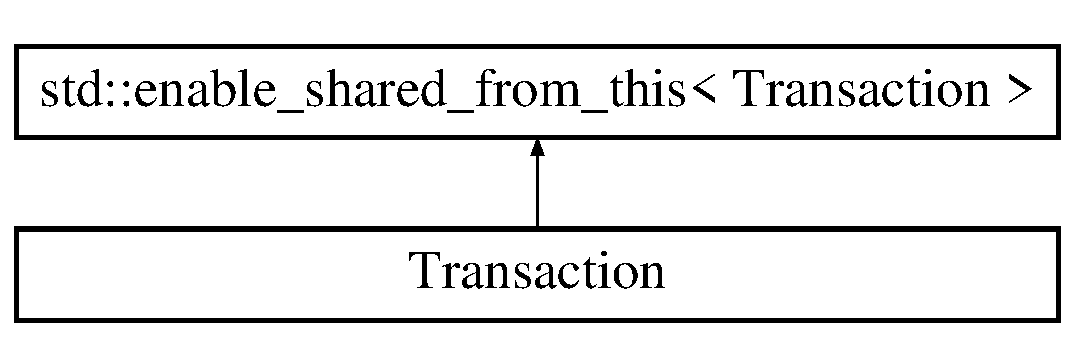
\includegraphics[height=2.000000cm]{classTransaction}
\end{center}
\end{figure}
\subsection*{Public Member Functions}
\begin{DoxyCompactItemize}
\item 
\mbox{\hyperlink{classTransaction_ab47005b855d38bc324bb79fd023baa13}{Transaction}} ()
\item 
\mbox{\hyperlink{classTransaction_a5a8028d0c89a04fbc5547806bfad7f4e}{Transaction}} (int ver, std\+::vector$<$ std\+::string $>$ initial\+Flags, std\+::vector$<$ \mbox{\hyperlink{structInputTransaction}{Input\+Transaction}} $>$ initial\+Inputs, std\+::vector$<$ \mbox{\hyperlink{structOutputTransaction}{Output\+Transaction}} $>$ initial\+Outputs)
\item 
\mbox{\hyperlink{classTransaction_a53699ce216993c3350d299aef80635d5}{Transaction}} (rapidjson\+::\+Document $\ast$doc)
\item 
int \mbox{\hyperlink{classTransaction_a133aff45373713e39a7a1317652dc55c}{get\+Version}} () const
\item 
std\+::vector$<$ std\+::string $>$ \mbox{\hyperlink{classTransaction_ab539d43c5af22bed8985473f26e8ac20}{get\+Flags}} () const
\item 
std\+::vector$<$ \mbox{\hyperlink{structTransactionIdentifier}{Transaction\+Identifier}} $>$ \mbox{\hyperlink{classTransaction_a0422efb4aea64a19437c350b04f7de96}{get\+Inputs\+Id}} () const
\item 
int \mbox{\hyperlink{classTransaction_abffdb9f040a484f89920842895d57ed2}{input\+Value}} (\mbox{\hyperlink{classMempool}{Mempool}} $\ast$mempool) const
\item 
int \mbox{\hyperlink{classTransaction_a1feb6131c4b683d6c59073dbf754a634}{output\+Value}} () const
\item 
int \mbox{\hyperlink{classTransaction_a490a7ae3f1520d95f9050ecc7197d1a0}{get\+Output\+Value}} (int index) const
\item 
bool \mbox{\hyperlink{classTransaction_aa2248446ed0d06f64d1685c386189666}{has\+Output}} (int index) const
\item 
int \mbox{\hyperlink{classTransaction_affdce860d7691f68b2e665a8f8d413fd}{get\+Output\+Number}} () const
\item 
bool \mbox{\hyperlink{classTransaction_a46f1d85f39193e516f795c3afe857c90}{check}} ()
\item 
bool \mbox{\hyperlink{classTransaction_afc37b00566ba0dc72e8efa9dd471601d}{validate}} (\mbox{\hyperlink{classMempool}{Mempool}} $\ast$mempool)
\item 
bool \mbox{\hyperlink{classTransaction_af326a5ba5ac0b525f326836423f3aa5f}{validate\+Script}} (\mbox{\hyperlink{classMempool}{Mempool}} $\ast$mempool) const
\item 
std\+::string \mbox{\hyperlink{classTransaction_a90b3668de562cc1b7f5773e72ac9f6dc}{raw\+Str}} () const
\item 
std\+::string \mbox{\hyperlink{classTransaction_a0f5aa15dc325b98730ba5eb786b0ffb2}{hash\+Without\+Inputs}} () const
\item 
std\+::string \mbox{\hyperlink{classTransaction_a99a851c61b60c1dd15b3e9bdd50f32f6}{hash}} () const
\item 
Value \mbox{\hyperlink{classTransaction_a41561665dfeef8f887fdc86f3c9849f8}{json}} (bool include\+Inputs, Document $\ast$document) const
\item 
std\+::string \mbox{\hyperlink{classTransaction_accf9cca56688761bdb9518c3f1b90ed5}{str}} () const
\end{DoxyCompactItemize}
\subsection*{Private Attributes}
\begin{DoxyCompactItemize}
\item 
int \mbox{\hyperlink{classTransaction_a7d8682b58b273ea2d0d6071355175ea3}{version}}
\item 
std\+::vector$<$ std\+::string $>$ \mbox{\hyperlink{classTransaction_afba77571560d1c92a2bb55a2adc4a9fc}{transaction\+Flags}}
\item 
std\+::vector$<$ \mbox{\hyperlink{structInputTransaction}{Input\+Transaction}} $>$ \mbox{\hyperlink{classTransaction_a3a4705bed22f34645476fd9642baf806}{inputs}}
\item 
std\+::vector$<$ \mbox{\hyperlink{structOutputTransaction}{Output\+Transaction}} $>$ \mbox{\hyperlink{classTransaction_a1a3d542cd9b8045e1256f128728fab37}{outputs}}
\end{DoxyCompactItemize}


\subsection{Constructor \& Destructor Documentation}
\mbox{\Hypertarget{classTransaction_ab47005b855d38bc324bb79fd023baa13}\label{classTransaction_ab47005b855d38bc324bb79fd023baa13}} 
\index{Transaction@{Transaction}!Transaction@{Transaction}}
\index{Transaction@{Transaction}!Transaction@{Transaction}}
\subsubsection{\texorpdfstring{Transaction()}{Transaction()}\hspace{0.1cm}{\footnotesize\ttfamily [1/3]}}
{\footnotesize\ttfamily Transaction\+::\+Transaction (\begin{DoxyParamCaption}{ }\end{DoxyParamCaption})}

\mbox{\Hypertarget{classTransaction_a5a8028d0c89a04fbc5547806bfad7f4e}\label{classTransaction_a5a8028d0c89a04fbc5547806bfad7f4e}} 
\index{Transaction@{Transaction}!Transaction@{Transaction}}
\index{Transaction@{Transaction}!Transaction@{Transaction}}
\subsubsection{\texorpdfstring{Transaction()}{Transaction()}\hspace{0.1cm}{\footnotesize\ttfamily [2/3]}}
{\footnotesize\ttfamily Transaction\+::\+Transaction (\begin{DoxyParamCaption}\item[{int}]{ver,  }\item[{std\+::vector$<$ std\+::string $>$}]{initial\+Flags,  }\item[{std\+::vector$<$ \mbox{\hyperlink{structInputTransaction}{Input\+Transaction}} $>$}]{initial\+Inputs,  }\item[{std\+::vector$<$ \mbox{\hyperlink{structOutputTransaction}{Output\+Transaction}} $>$}]{initial\+Outputs }\end{DoxyParamCaption})}

\mbox{\Hypertarget{classTransaction_a53699ce216993c3350d299aef80635d5}\label{classTransaction_a53699ce216993c3350d299aef80635d5}} 
\index{Transaction@{Transaction}!Transaction@{Transaction}}
\index{Transaction@{Transaction}!Transaction@{Transaction}}
\subsubsection{\texorpdfstring{Transaction()}{Transaction()}\hspace{0.1cm}{\footnotesize\ttfamily [3/3]}}
{\footnotesize\ttfamily Transaction\+::\+Transaction (\begin{DoxyParamCaption}\item[{rapidjson\+::\+Document $\ast$}]{doc }\end{DoxyParamCaption})\hspace{0.3cm}{\ttfamily [explicit]}}



\subsection{Member Function Documentation}
\mbox{\Hypertarget{classTransaction_a46f1d85f39193e516f795c3afe857c90}\label{classTransaction_a46f1d85f39193e516f795c3afe857c90}} 
\index{Transaction@{Transaction}!check@{check}}
\index{check@{check}!Transaction@{Transaction}}
\subsubsection{\texorpdfstring{check()}{check()}}
{\footnotesize\ttfamily bool Transaction\+::check (\begin{DoxyParamCaption}{ }\end{DoxyParamCaption})}

\mbox{\Hypertarget{classTransaction_ab539d43c5af22bed8985473f26e8ac20}\label{classTransaction_ab539d43c5af22bed8985473f26e8ac20}} 
\index{Transaction@{Transaction}!get\+Flags@{get\+Flags}}
\index{get\+Flags@{get\+Flags}!Transaction@{Transaction}}
\subsubsection{\texorpdfstring{get\+Flags()}{getFlags()}}
{\footnotesize\ttfamily std\+::vector$<$ std\+::string $>$ Transaction\+::get\+Flags (\begin{DoxyParamCaption}{ }\end{DoxyParamCaption}) const}

\mbox{\Hypertarget{classTransaction_a0422efb4aea64a19437c350b04f7de96}\label{classTransaction_a0422efb4aea64a19437c350b04f7de96}} 
\index{Transaction@{Transaction}!get\+Inputs\+Id@{get\+Inputs\+Id}}
\index{get\+Inputs\+Id@{get\+Inputs\+Id}!Transaction@{Transaction}}
\subsubsection{\texorpdfstring{get\+Inputs\+Id()}{getInputsId()}}
{\footnotesize\ttfamily std\+::vector$<$ \mbox{\hyperlink{structTransactionIdentifier}{Transaction\+Identifier}} $>$ Transaction\+::get\+Inputs\+Id (\begin{DoxyParamCaption}{ }\end{DoxyParamCaption}) const}

\mbox{\Hypertarget{classTransaction_affdce860d7691f68b2e665a8f8d413fd}\label{classTransaction_affdce860d7691f68b2e665a8f8d413fd}} 
\index{Transaction@{Transaction}!get\+Output\+Number@{get\+Output\+Number}}
\index{get\+Output\+Number@{get\+Output\+Number}!Transaction@{Transaction}}
\subsubsection{\texorpdfstring{get\+Output\+Number()}{getOutputNumber()}}
{\footnotesize\ttfamily int Transaction\+::get\+Output\+Number (\begin{DoxyParamCaption}{ }\end{DoxyParamCaption}) const}

\mbox{\Hypertarget{classTransaction_a490a7ae3f1520d95f9050ecc7197d1a0}\label{classTransaction_a490a7ae3f1520d95f9050ecc7197d1a0}} 
\index{Transaction@{Transaction}!get\+Output\+Value@{get\+Output\+Value}}
\index{get\+Output\+Value@{get\+Output\+Value}!Transaction@{Transaction}}
\subsubsection{\texorpdfstring{get\+Output\+Value()}{getOutputValue()}}
{\footnotesize\ttfamily int Transaction\+::get\+Output\+Value (\begin{DoxyParamCaption}\item[{int}]{index }\end{DoxyParamCaption}) const}

\mbox{\Hypertarget{classTransaction_a133aff45373713e39a7a1317652dc55c}\label{classTransaction_a133aff45373713e39a7a1317652dc55c}} 
\index{Transaction@{Transaction}!get\+Version@{get\+Version}}
\index{get\+Version@{get\+Version}!Transaction@{Transaction}}
\subsubsection{\texorpdfstring{get\+Version()}{getVersion()}}
{\footnotesize\ttfamily int Transaction\+::get\+Version (\begin{DoxyParamCaption}{ }\end{DoxyParamCaption}) const}

\mbox{\Hypertarget{classTransaction_a99a851c61b60c1dd15b3e9bdd50f32f6}\label{classTransaction_a99a851c61b60c1dd15b3e9bdd50f32f6}} 
\index{Transaction@{Transaction}!hash@{hash}}
\index{hash@{hash}!Transaction@{Transaction}}
\subsubsection{\texorpdfstring{hash()}{hash()}}
{\footnotesize\ttfamily std\+::string Transaction\+::hash (\begin{DoxyParamCaption}{ }\end{DoxyParamCaption}) const}

\mbox{\Hypertarget{classTransaction_a0f5aa15dc325b98730ba5eb786b0ffb2}\label{classTransaction_a0f5aa15dc325b98730ba5eb786b0ffb2}} 
\index{Transaction@{Transaction}!hash\+Without\+Inputs@{hash\+Without\+Inputs}}
\index{hash\+Without\+Inputs@{hash\+Without\+Inputs}!Transaction@{Transaction}}
\subsubsection{\texorpdfstring{hash\+Without\+Inputs()}{hashWithoutInputs()}}
{\footnotesize\ttfamily std\+::string Transaction\+::hash\+Without\+Inputs (\begin{DoxyParamCaption}{ }\end{DoxyParamCaption}) const}

\mbox{\Hypertarget{classTransaction_aa2248446ed0d06f64d1685c386189666}\label{classTransaction_aa2248446ed0d06f64d1685c386189666}} 
\index{Transaction@{Transaction}!has\+Output@{has\+Output}}
\index{has\+Output@{has\+Output}!Transaction@{Transaction}}
\subsubsection{\texorpdfstring{has\+Output()}{hasOutput()}}
{\footnotesize\ttfamily bool Transaction\+::has\+Output (\begin{DoxyParamCaption}\item[{int}]{index }\end{DoxyParamCaption}) const}

\mbox{\Hypertarget{classTransaction_abffdb9f040a484f89920842895d57ed2}\label{classTransaction_abffdb9f040a484f89920842895d57ed2}} 
\index{Transaction@{Transaction}!input\+Value@{input\+Value}}
\index{input\+Value@{input\+Value}!Transaction@{Transaction}}
\subsubsection{\texorpdfstring{input\+Value()}{inputValue()}}
{\footnotesize\ttfamily int Transaction\+::input\+Value (\begin{DoxyParamCaption}\item[{\mbox{\hyperlink{classMempool}{Mempool}} $\ast$}]{mempool }\end{DoxyParamCaption}) const}

\mbox{\Hypertarget{classTransaction_a41561665dfeef8f887fdc86f3c9849f8}\label{classTransaction_a41561665dfeef8f887fdc86f3c9849f8}} 
\index{Transaction@{Transaction}!json@{json}}
\index{json@{json}!Transaction@{Transaction}}
\subsubsection{\texorpdfstring{json()}{json()}}
{\footnotesize\ttfamily Value Transaction\+::json (\begin{DoxyParamCaption}\item[{bool}]{include\+Inputs,  }\item[{Document $\ast$}]{document }\end{DoxyParamCaption}) const}

\mbox{\Hypertarget{classTransaction_a1feb6131c4b683d6c59073dbf754a634}\label{classTransaction_a1feb6131c4b683d6c59073dbf754a634}} 
\index{Transaction@{Transaction}!output\+Value@{output\+Value}}
\index{output\+Value@{output\+Value}!Transaction@{Transaction}}
\subsubsection{\texorpdfstring{output\+Value()}{outputValue()}}
{\footnotesize\ttfamily int Transaction\+::output\+Value (\begin{DoxyParamCaption}{ }\end{DoxyParamCaption}) const}

\mbox{\Hypertarget{classTransaction_a90b3668de562cc1b7f5773e72ac9f6dc}\label{classTransaction_a90b3668de562cc1b7f5773e72ac9f6dc}} 
\index{Transaction@{Transaction}!raw\+Str@{raw\+Str}}
\index{raw\+Str@{raw\+Str}!Transaction@{Transaction}}
\subsubsection{\texorpdfstring{raw\+Str()}{rawStr()}}
{\footnotesize\ttfamily std\+::string Transaction\+::raw\+Str (\begin{DoxyParamCaption}{ }\end{DoxyParamCaption}) const}

\mbox{\Hypertarget{classTransaction_accf9cca56688761bdb9518c3f1b90ed5}\label{classTransaction_accf9cca56688761bdb9518c3f1b90ed5}} 
\index{Transaction@{Transaction}!str@{str}}
\index{str@{str}!Transaction@{Transaction}}
\subsubsection{\texorpdfstring{str()}{str()}}
{\footnotesize\ttfamily std\+::string Transaction\+::str (\begin{DoxyParamCaption}{ }\end{DoxyParamCaption}) const}

\mbox{\Hypertarget{classTransaction_afc37b00566ba0dc72e8efa9dd471601d}\label{classTransaction_afc37b00566ba0dc72e8efa9dd471601d}} 
\index{Transaction@{Transaction}!validate@{validate}}
\index{validate@{validate}!Transaction@{Transaction}}
\subsubsection{\texorpdfstring{validate()}{validate()}}
{\footnotesize\ttfamily bool Transaction\+::validate (\begin{DoxyParamCaption}\item[{\mbox{\hyperlink{classMempool}{Mempool}} $\ast$}]{mempool }\end{DoxyParamCaption})}

\mbox{\Hypertarget{classTransaction_af326a5ba5ac0b525f326836423f3aa5f}\label{classTransaction_af326a5ba5ac0b525f326836423f3aa5f}} 
\index{Transaction@{Transaction}!validate\+Script@{validate\+Script}}
\index{validate\+Script@{validate\+Script}!Transaction@{Transaction}}
\subsubsection{\texorpdfstring{validate\+Script()}{validateScript()}}
{\footnotesize\ttfamily bool Transaction\+::validate\+Script (\begin{DoxyParamCaption}\item[{\mbox{\hyperlink{classMempool}{Mempool}} $\ast$}]{mempool }\end{DoxyParamCaption}) const}



\subsection{Member Data Documentation}
\mbox{\Hypertarget{classTransaction_a3a4705bed22f34645476fd9642baf806}\label{classTransaction_a3a4705bed22f34645476fd9642baf806}} 
\index{Transaction@{Transaction}!inputs@{inputs}}
\index{inputs@{inputs}!Transaction@{Transaction}}
\subsubsection{\texorpdfstring{inputs}{inputs}}
{\footnotesize\ttfamily std\+::vector$<$\mbox{\hyperlink{structInputTransaction}{Input\+Transaction}}$>$ Transaction\+::inputs\hspace{0.3cm}{\ttfamily [private]}}

\mbox{\Hypertarget{classTransaction_a1a3d542cd9b8045e1256f128728fab37}\label{classTransaction_a1a3d542cd9b8045e1256f128728fab37}} 
\index{Transaction@{Transaction}!outputs@{outputs}}
\index{outputs@{outputs}!Transaction@{Transaction}}
\subsubsection{\texorpdfstring{outputs}{outputs}}
{\footnotesize\ttfamily std\+::vector$<$\mbox{\hyperlink{structOutputTransaction}{Output\+Transaction}}$>$ Transaction\+::outputs\hspace{0.3cm}{\ttfamily [private]}}

\mbox{\Hypertarget{classTransaction_afba77571560d1c92a2bb55a2adc4a9fc}\label{classTransaction_afba77571560d1c92a2bb55a2adc4a9fc}} 
\index{Transaction@{Transaction}!transaction\+Flags@{transaction\+Flags}}
\index{transaction\+Flags@{transaction\+Flags}!Transaction@{Transaction}}
\subsubsection{\texorpdfstring{transaction\+Flags}{transactionFlags}}
{\footnotesize\ttfamily std\+::vector$<$std\+::string$>$ Transaction\+::transaction\+Flags\hspace{0.3cm}{\ttfamily [private]}}

\mbox{\Hypertarget{classTransaction_a7d8682b58b273ea2d0d6071355175ea3}\label{classTransaction_a7d8682b58b273ea2d0d6071355175ea3}} 
\index{Transaction@{Transaction}!version@{version}}
\index{version@{version}!Transaction@{Transaction}}
\subsubsection{\texorpdfstring{version}{version}}
{\footnotesize\ttfamily int Transaction\+::version\hspace{0.3cm}{\ttfamily [private]}}



The documentation for this class was generated from the following files\+:\begin{DoxyCompactItemize}
\item 
include/\mbox{\hyperlink{transaction_8hpp}{transaction.\+hpp}}\item 
src/transaction/\mbox{\hyperlink{transaction_8cpp}{transaction.\+cpp}}\end{DoxyCompactItemize}

\hypertarget{structTransactionIdentifier}{}\section{Transaction\+Identifier Struct Reference}
\label{structTransactionIdentifier}\index{Transaction\+Identifier@{Transaction\+Identifier}}


{\ttfamily \#include $<$transaction.\+hpp$>$}

\subsection*{Public Member Functions}
\begin{DoxyCompactItemize}
\item 
std\+::string \mbox{\hyperlink{structTransactionIdentifier_a00d46c50b8e79327f4c3b9bc32a7f679}{str}} () const
\item 
Value \mbox{\hyperlink{structTransactionIdentifier_ab8879716182a6beddfc4093e73703324}{json}} (Document $\ast$document) const
\item 
void \mbox{\hyperlink{structTransactionIdentifier_a0f109058df0aa00717a1acdc10fbc97e}{load}} (Value $\ast$val)
\end{DoxyCompactItemize}
\subsection*{Public Attributes}
\begin{DoxyCompactItemize}
\item 
std\+::string \mbox{\hyperlink{structTransactionIdentifier_a4fbb1245879f1cccdc27b64ad7f0cbac}{transaction\+Hash}}
\item 
int \mbox{\hyperlink{structTransactionIdentifier_a667fa04ae76976ba5b3940621fb5f8ad}{index}}
\end{DoxyCompactItemize}


\subsection{Member Function Documentation}
\mbox{\Hypertarget{structTransactionIdentifier_ab8879716182a6beddfc4093e73703324}\label{structTransactionIdentifier_ab8879716182a6beddfc4093e73703324}} 
\index{Transaction\+Identifier@{Transaction\+Identifier}!json@{json}}
\index{json@{json}!Transaction\+Identifier@{Transaction\+Identifier}}
\subsubsection{\texorpdfstring{json()}{json()}}
{\footnotesize\ttfamily Value Transaction\+Identifier\+::json (\begin{DoxyParamCaption}\item[{Document $\ast$}]{document }\end{DoxyParamCaption}) const}

\mbox{\Hypertarget{structTransactionIdentifier_a0f109058df0aa00717a1acdc10fbc97e}\label{structTransactionIdentifier_a0f109058df0aa00717a1acdc10fbc97e}} 
\index{Transaction\+Identifier@{Transaction\+Identifier}!load@{load}}
\index{load@{load}!Transaction\+Identifier@{Transaction\+Identifier}}
\subsubsection{\texorpdfstring{load()}{load()}}
{\footnotesize\ttfamily void Transaction\+Identifier\+::load (\begin{DoxyParamCaption}\item[{Value $\ast$}]{val }\end{DoxyParamCaption})}

\mbox{\Hypertarget{structTransactionIdentifier_a00d46c50b8e79327f4c3b9bc32a7f679}\label{structTransactionIdentifier_a00d46c50b8e79327f4c3b9bc32a7f679}} 
\index{Transaction\+Identifier@{Transaction\+Identifier}!str@{str}}
\index{str@{str}!Transaction\+Identifier@{Transaction\+Identifier}}
\subsubsection{\texorpdfstring{str()}{str()}}
{\footnotesize\ttfamily std\+::string Transaction\+Identifier\+::str (\begin{DoxyParamCaption}{ }\end{DoxyParamCaption}) const}



\subsection{Member Data Documentation}
\mbox{\Hypertarget{structTransactionIdentifier_a667fa04ae76976ba5b3940621fb5f8ad}\label{structTransactionIdentifier_a667fa04ae76976ba5b3940621fb5f8ad}} 
\index{Transaction\+Identifier@{Transaction\+Identifier}!index@{index}}
\index{index@{index}!Transaction\+Identifier@{Transaction\+Identifier}}
\subsubsection{\texorpdfstring{index}{index}}
{\footnotesize\ttfamily int Transaction\+Identifier\+::index}

\mbox{\Hypertarget{structTransactionIdentifier_a4fbb1245879f1cccdc27b64ad7f0cbac}\label{structTransactionIdentifier_a4fbb1245879f1cccdc27b64ad7f0cbac}} 
\index{Transaction\+Identifier@{Transaction\+Identifier}!transaction\+Hash@{transaction\+Hash}}
\index{transaction\+Hash@{transaction\+Hash}!Transaction\+Identifier@{Transaction\+Identifier}}
\subsubsection{\texorpdfstring{transaction\+Hash}{transactionHash}}
{\footnotesize\ttfamily std\+::string Transaction\+Identifier\+::transaction\+Hash}



The documentation for this struct was generated from the following files\+:\begin{DoxyCompactItemize}
\item 
include/\mbox{\hyperlink{transaction_8hpp}{transaction.\+hpp}}\item 
src/transaction/\mbox{\hyperlink{transactionid_8cpp}{transactionid.\+cpp}}\end{DoxyCompactItemize}

\hypertarget{classTransactionMessage}{}\section{Transaction\+Message Class Reference}
\label{classTransactionMessage}\index{Transaction\+Message@{Transaction\+Message}}


{\ttfamily \#include $<$messages.\+hpp$>$}

Inheritance diagram for Transaction\+Message\+:\begin{figure}[H]
\begin{center}
\leavevmode
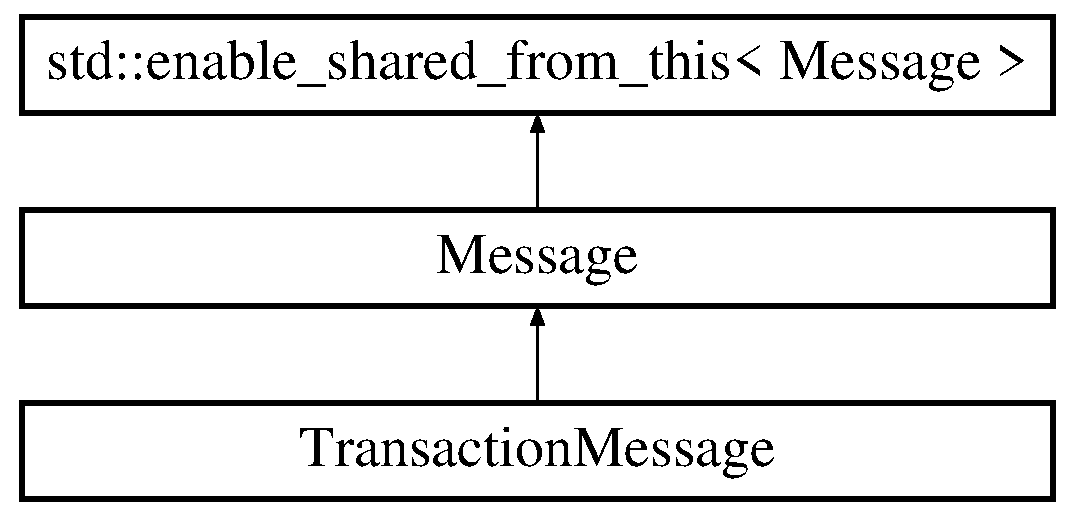
\includegraphics[height=3.000000cm]{classTransactionMessage}
\end{center}
\end{figure}
\subsection*{Public Member Functions}
\begin{DoxyCompactItemize}
\item 
\mbox{\hyperlink{classTransactionMessage_a8bb90fe0dc9dba6de05f27772f03c708}{Transaction\+Message}} (std\+::shared\+\_\+ptr$<$ \mbox{\hyperlink{classTransaction}{Transaction}} $>$ tr\+Ptr)
\item 
\mbox{\hyperlink{classTransactionMessage_a767282698bcd84202aa9eb59ef4feb2d}{Transaction\+Message}} (rapidjson\+::\+Document $\ast$doc)
\item 
rapidjson\+::\+Value \mbox{\hyperlink{classTransactionMessage_af8675087bd26b6aa0c30a3e3141dda4e}{json}} (rapidjson\+::\+Document $\ast$doc) const override
\end{DoxyCompactItemize}
\subsection*{Private Attributes}
\begin{DoxyCompactItemize}
\item 
std\+::shared\+\_\+ptr$<$ \mbox{\hyperlink{classTransaction}{Transaction}} $>$ \mbox{\hyperlink{classTransactionMessage_a5949ed4449ab8031ffc6342268b981ff}{transaction}}
\end{DoxyCompactItemize}
\subsection*{Additional Inherited Members}


\subsection{Constructor \& Destructor Documentation}
\mbox{\Hypertarget{classTransactionMessage_a8bb90fe0dc9dba6de05f27772f03c708}\label{classTransactionMessage_a8bb90fe0dc9dba6de05f27772f03c708}} 
\index{Transaction\+Message@{Transaction\+Message}!Transaction\+Message@{Transaction\+Message}}
\index{Transaction\+Message@{Transaction\+Message}!Transaction\+Message@{Transaction\+Message}}
\subsubsection{\texorpdfstring{Transaction\+Message()}{TransactionMessage()}\hspace{0.1cm}{\footnotesize\ttfamily [1/2]}}
{\footnotesize\ttfamily Transaction\+Message\+::\+Transaction\+Message (\begin{DoxyParamCaption}\item[{std\+::shared\+\_\+ptr$<$ \mbox{\hyperlink{classTransaction}{Transaction}} $>$}]{tr\+Ptr }\end{DoxyParamCaption})\hspace{0.3cm}{\ttfamily [explicit]}}

\mbox{\Hypertarget{classTransactionMessage_a767282698bcd84202aa9eb59ef4feb2d}\label{classTransactionMessage_a767282698bcd84202aa9eb59ef4feb2d}} 
\index{Transaction\+Message@{Transaction\+Message}!Transaction\+Message@{Transaction\+Message}}
\index{Transaction\+Message@{Transaction\+Message}!Transaction\+Message@{Transaction\+Message}}
\subsubsection{\texorpdfstring{Transaction\+Message()}{TransactionMessage()}\hspace{0.1cm}{\footnotesize\ttfamily [2/2]}}
{\footnotesize\ttfamily Transaction\+Message\+::\+Transaction\+Message (\begin{DoxyParamCaption}\item[{rapidjson\+::\+Document $\ast$}]{doc }\end{DoxyParamCaption})\hspace{0.3cm}{\ttfamily [explicit]}}



\subsection{Member Function Documentation}
\mbox{\Hypertarget{classTransactionMessage_af8675087bd26b6aa0c30a3e3141dda4e}\label{classTransactionMessage_af8675087bd26b6aa0c30a3e3141dda4e}} 
\index{Transaction\+Message@{Transaction\+Message}!json@{json}}
\index{json@{json}!Transaction\+Message@{Transaction\+Message}}
\subsubsection{\texorpdfstring{json()}{json()}}
{\footnotesize\ttfamily rapidjson\+::\+Value Transaction\+Message\+::json (\begin{DoxyParamCaption}\item[{rapidjson\+::\+Document $\ast$}]{doc }\end{DoxyParamCaption}) const\hspace{0.3cm}{\ttfamily [override]}, {\ttfamily [virtual]}}



Reimplemented from \mbox{\hyperlink{classMessage_a6f8e3ac2eed3a8afe9400fcd5b3447b2}{Message}}.



\subsection{Member Data Documentation}
\mbox{\Hypertarget{classTransactionMessage_a5949ed4449ab8031ffc6342268b981ff}\label{classTransactionMessage_a5949ed4449ab8031ffc6342268b981ff}} 
\index{Transaction\+Message@{Transaction\+Message}!transaction@{transaction}}
\index{transaction@{transaction}!Transaction\+Message@{Transaction\+Message}}
\subsubsection{\texorpdfstring{transaction}{transaction}}
{\footnotesize\ttfamily std\+::shared\+\_\+ptr$<$\mbox{\hyperlink{classTransaction}{Transaction}}$>$ Transaction\+Message\+::transaction\hspace{0.3cm}{\ttfamily [private]}}



The documentation for this class was generated from the following files\+:\begin{DoxyCompactItemize}
\item 
include/\mbox{\hyperlink{messages_8hpp}{messages.\+hpp}}\item 
src/message/\mbox{\hyperlink{transactionmessage_8cpp}{transactionmessage.\+cpp}}\end{DoxyCompactItemize}

\hypertarget{structUTXOdata}{}\section{U\+T\+X\+Odata Struct Reference}
\label{structUTXOdata}\index{U\+T\+X\+Odata@{U\+T\+X\+Odata}}


{\ttfamily \#include $<$utxo.\+hpp$>$}

\subsection*{Public Member Functions}
\begin{DoxyCompactItemize}
\item 
\mbox{\hyperlink{structUTXOdata_abac0ce6dfed6dab29a00a995d37cc62c}{U\+T\+X\+Odata}} (int, bool)
\item 
\mbox{\hyperlink{structUTXOdata_a0f569e3b932610a822140104fdd418a9}{U\+T\+X\+Odata}} (std\+::string json\+Str)
\item 
std\+::string \mbox{\hyperlink{structUTXOdata_a8416d6a4cc715159a8e2f9da47b5519a}{str}} () const
\end{DoxyCompactItemize}
\subsection*{Public Attributes}
\begin{DoxyCompactItemize}
\item 
int \mbox{\hyperlink{structUTXOdata_a255dc301eba5d915c6a5dc752ec11a86}{value}}
\item 
bool \mbox{\hyperlink{structUTXOdata_aec980c11dde6738bf2120fb3bd3e541f}{coinbase}}
\item 
int \mbox{\hyperlink{structUTXOdata_ac437a55d55e7d7de1bd2558fefccc541}{height}}
\item 
std\+::string \mbox{\hyperlink{structUTXOdata_ae2bfbc7be65eb1c5583084572818ddb2}{hash\+Without\+Inputs}}
\item 
std\+::vector$<$ std\+::string $>$ \mbox{\hyperlink{structUTXOdata_a9195f06da49760fd982965b008f906c2}{script}}
\end{DoxyCompactItemize}


\subsection{Constructor \& Destructor Documentation}
\mbox{\Hypertarget{structUTXOdata_abac0ce6dfed6dab29a00a995d37cc62c}\label{structUTXOdata_abac0ce6dfed6dab29a00a995d37cc62c}} 
\index{U\+T\+X\+Odata@{U\+T\+X\+Odata}!U\+T\+X\+Odata@{U\+T\+X\+Odata}}
\index{U\+T\+X\+Odata@{U\+T\+X\+Odata}!U\+T\+X\+Odata@{U\+T\+X\+Odata}}
\subsubsection{\texorpdfstring{U\+T\+X\+Odata()}{UTXOdata()}\hspace{0.1cm}{\footnotesize\ttfamily [1/2]}}
{\footnotesize\ttfamily U\+T\+X\+Odata\+::\+U\+T\+X\+Odata (\begin{DoxyParamCaption}\item[{int}]{val,  }\item[{bool}]{cb }\end{DoxyParamCaption})}

\mbox{\Hypertarget{structUTXOdata_a0f569e3b932610a822140104fdd418a9}\label{structUTXOdata_a0f569e3b932610a822140104fdd418a9}} 
\index{U\+T\+X\+Odata@{U\+T\+X\+Odata}!U\+T\+X\+Odata@{U\+T\+X\+Odata}}
\index{U\+T\+X\+Odata@{U\+T\+X\+Odata}!U\+T\+X\+Odata@{U\+T\+X\+Odata}}
\subsubsection{\texorpdfstring{U\+T\+X\+Odata()}{UTXOdata()}\hspace{0.1cm}{\footnotesize\ttfamily [2/2]}}
{\footnotesize\ttfamily U\+T\+X\+Odata\+::\+U\+T\+X\+Odata (\begin{DoxyParamCaption}\item[{std\+::string}]{json\+Str }\end{DoxyParamCaption})\hspace{0.3cm}{\ttfamily [explicit]}}



\subsection{Member Function Documentation}
\mbox{\Hypertarget{structUTXOdata_a8416d6a4cc715159a8e2f9da47b5519a}\label{structUTXOdata_a8416d6a4cc715159a8e2f9da47b5519a}} 
\index{U\+T\+X\+Odata@{U\+T\+X\+Odata}!str@{str}}
\index{str@{str}!U\+T\+X\+Odata@{U\+T\+X\+Odata}}
\subsubsection{\texorpdfstring{str()}{str()}}
{\footnotesize\ttfamily std\+::string U\+T\+X\+Odata\+::str (\begin{DoxyParamCaption}{ }\end{DoxyParamCaption}) const}



\subsection{Member Data Documentation}
\mbox{\Hypertarget{structUTXOdata_aec980c11dde6738bf2120fb3bd3e541f}\label{structUTXOdata_aec980c11dde6738bf2120fb3bd3e541f}} 
\index{U\+T\+X\+Odata@{U\+T\+X\+Odata}!coinbase@{coinbase}}
\index{coinbase@{coinbase}!U\+T\+X\+Odata@{U\+T\+X\+Odata}}
\subsubsection{\texorpdfstring{coinbase}{coinbase}}
{\footnotesize\ttfamily bool U\+T\+X\+Odata\+::coinbase}

\mbox{\Hypertarget{structUTXOdata_ae2bfbc7be65eb1c5583084572818ddb2}\label{structUTXOdata_ae2bfbc7be65eb1c5583084572818ddb2}} 
\index{U\+T\+X\+Odata@{U\+T\+X\+Odata}!hash\+Without\+Inputs@{hash\+Without\+Inputs}}
\index{hash\+Without\+Inputs@{hash\+Without\+Inputs}!U\+T\+X\+Odata@{U\+T\+X\+Odata}}
\subsubsection{\texorpdfstring{hash\+Without\+Inputs}{hashWithoutInputs}}
{\footnotesize\ttfamily std\+::string U\+T\+X\+Odata\+::hash\+Without\+Inputs}

\mbox{\Hypertarget{structUTXOdata_ac437a55d55e7d7de1bd2558fefccc541}\label{structUTXOdata_ac437a55d55e7d7de1bd2558fefccc541}} 
\index{U\+T\+X\+Odata@{U\+T\+X\+Odata}!height@{height}}
\index{height@{height}!U\+T\+X\+Odata@{U\+T\+X\+Odata}}
\subsubsection{\texorpdfstring{height}{height}}
{\footnotesize\ttfamily int U\+T\+X\+Odata\+::height}

\mbox{\Hypertarget{structUTXOdata_a9195f06da49760fd982965b008f906c2}\label{structUTXOdata_a9195f06da49760fd982965b008f906c2}} 
\index{U\+T\+X\+Odata@{U\+T\+X\+Odata}!script@{script}}
\index{script@{script}!U\+T\+X\+Odata@{U\+T\+X\+Odata}}
\subsubsection{\texorpdfstring{script}{script}}
{\footnotesize\ttfamily std\+::vector$<$std\+::string$>$ U\+T\+X\+Odata\+::script}

\mbox{\Hypertarget{structUTXOdata_a255dc301eba5d915c6a5dc752ec11a86}\label{structUTXOdata_a255dc301eba5d915c6a5dc752ec11a86}} 
\index{U\+T\+X\+Odata@{U\+T\+X\+Odata}!value@{value}}
\index{value@{value}!U\+T\+X\+Odata@{U\+T\+X\+Odata}}
\subsubsection{\texorpdfstring{value}{value}}
{\footnotesize\ttfamily int U\+T\+X\+Odata\+::value}



The documentation for this struct was generated from the following files\+:\begin{DoxyCompactItemize}
\item 
include/\mbox{\hyperlink{utxo_8hpp}{utxo.\+hpp}}\item 
src/\mbox{\hyperlink{utxo_8cpp}{utxo.\+cpp}}\end{DoxyCompactItemize}

\hypertarget{classUTXOManager}{}\section{U\+T\+X\+O\+Manager Class Reference}
\label{classUTXOManager}\index{U\+T\+X\+O\+Manager@{U\+T\+X\+O\+Manager}}


{\ttfamily \#include $<$utxo.\+hpp$>$}

\subsection*{Public Member Functions}
\begin{DoxyCompactItemize}
\item 
\mbox{\hyperlink{classUTXOManager_aa08c4e17616d0a2436df1c8307b5da26}{U\+T\+X\+O\+Manager}} ()
\item 
int \mbox{\hyperlink{classUTXOManager_ae326f42b81d5d21b5232b715e7cef076}{get\+Value}} (\mbox{\hyperlink{utxo_8hpp_a19091d002da03ec92277e19295ac4540}{U\+T\+XO}} id) const
\item 
bool \mbox{\hyperlink{classUTXOManager_a4bcd0b36baf1ed245c48a826db241345}{is\+Coinbase}} (\mbox{\hyperlink{utxo_8hpp_a19091d002da03ec92277e19295ac4540}{U\+T\+XO}} id) const
\item 
int \mbox{\hyperlink{classUTXOManager_a4ae666af31dc1be4bd160a179aeef2ce}{get\+Height}} (\mbox{\hyperlink{utxo_8hpp_a19091d002da03ec92277e19295ac4540}{U\+T\+XO}} id) const
\item 
std\+::vector$<$ std\+::string $>$ \mbox{\hyperlink{classUTXOManager_a156c895274840fa2c6c93fead39b38e5}{get\+Output\+Script}} (\mbox{\hyperlink{utxo_8hpp_a19091d002da03ec92277e19295ac4540}{U\+T\+XO}} id) const
\item 
std\+::string \mbox{\hyperlink{classUTXOManager_acfad0e67f3b475bd4d6a9fd0fb977e6a}{get\+Hash\+Signature}} (\mbox{\hyperlink{utxo_8hpp_a19091d002da03ec92277e19295ac4540}{U\+T\+XO}} id) const
\item 
bool \mbox{\hyperlink{classUTXOManager_a599c57b261e313bd99a3783e1ad7def5}{exists}} (\mbox{\hyperlink{utxo_8hpp_a19091d002da03ec92277e19295ac4540}{U\+T\+XO}} id) const
\item 
void \mbox{\hyperlink{classUTXOManager_ab0ed356ad058c35e0bd4f97a8eb34380}{add}} (\mbox{\hyperlink{utxo_8hpp_a19091d002da03ec92277e19295ac4540}{U\+T\+XO}} id, \mbox{\hyperlink{structUTXOdata}{U\+T\+X\+Odata}} data)
\item 
void \mbox{\hyperlink{classUTXOManager_af08863b6400556a6350b3d7122cd1dc4}{spend}} (\mbox{\hyperlink{utxo_8hpp_a19091d002da03ec92277e19295ac4540}{U\+T\+XO}} txid)
\end{DoxyCompactItemize}
\subsection*{Private Member Functions}
\begin{DoxyCompactItemize}
\item 
\mbox{\hyperlink{structUTXOdata}{U\+T\+X\+Odata}} \mbox{\hyperlink{classUTXOManager_a7aabe910f5f8d24604d33429f5d4bafd}{get\+Data}} (\mbox{\hyperlink{utxo_8hpp_a19091d002da03ec92277e19295ac4540}{U\+T\+XO}} id) const
\end{DoxyCompactItemize}
\subsection*{Private Attributes}
\begin{DoxyCompactItemize}
\item 
leveldb\+::\+DB $\ast$ \mbox{\hyperlink{classUTXOManager_a41e7280e7d1384aca9dbf2e15b1085cf}{db}}
\end{DoxyCompactItemize}


\subsection{Constructor \& Destructor Documentation}
\mbox{\Hypertarget{classUTXOManager_aa08c4e17616d0a2436df1c8307b5da26}\label{classUTXOManager_aa08c4e17616d0a2436df1c8307b5da26}} 
\index{U\+T\+X\+O\+Manager@{U\+T\+X\+O\+Manager}!U\+T\+X\+O\+Manager@{U\+T\+X\+O\+Manager}}
\index{U\+T\+X\+O\+Manager@{U\+T\+X\+O\+Manager}!U\+T\+X\+O\+Manager@{U\+T\+X\+O\+Manager}}
\subsubsection{\texorpdfstring{U\+T\+X\+O\+Manager()}{UTXOManager()}}
{\footnotesize\ttfamily U\+T\+X\+O\+Manager\+::\+U\+T\+X\+O\+Manager (\begin{DoxyParamCaption}{ }\end{DoxyParamCaption})}



\subsection{Member Function Documentation}
\mbox{\Hypertarget{classUTXOManager_ab0ed356ad058c35e0bd4f97a8eb34380}\label{classUTXOManager_ab0ed356ad058c35e0bd4f97a8eb34380}} 
\index{U\+T\+X\+O\+Manager@{U\+T\+X\+O\+Manager}!add@{add}}
\index{add@{add}!U\+T\+X\+O\+Manager@{U\+T\+X\+O\+Manager}}
\subsubsection{\texorpdfstring{add()}{add()}}
{\footnotesize\ttfamily void U\+T\+X\+O\+Manager\+::add (\begin{DoxyParamCaption}\item[{\mbox{\hyperlink{utxo_8hpp_a19091d002da03ec92277e19295ac4540}{U\+T\+XO}}}]{id,  }\item[{\mbox{\hyperlink{structUTXOdata}{U\+T\+X\+Odata}}}]{data }\end{DoxyParamCaption})}

\mbox{\Hypertarget{classUTXOManager_a599c57b261e313bd99a3783e1ad7def5}\label{classUTXOManager_a599c57b261e313bd99a3783e1ad7def5}} 
\index{U\+T\+X\+O\+Manager@{U\+T\+X\+O\+Manager}!exists@{exists}}
\index{exists@{exists}!U\+T\+X\+O\+Manager@{U\+T\+X\+O\+Manager}}
\subsubsection{\texorpdfstring{exists()}{exists()}}
{\footnotesize\ttfamily bool U\+T\+X\+O\+Manager\+::exists (\begin{DoxyParamCaption}\item[{\mbox{\hyperlink{utxo_8hpp_a19091d002da03ec92277e19295ac4540}{U\+T\+XO}}}]{id }\end{DoxyParamCaption}) const}

\mbox{\Hypertarget{classUTXOManager_a7aabe910f5f8d24604d33429f5d4bafd}\label{classUTXOManager_a7aabe910f5f8d24604d33429f5d4bafd}} 
\index{U\+T\+X\+O\+Manager@{U\+T\+X\+O\+Manager}!get\+Data@{get\+Data}}
\index{get\+Data@{get\+Data}!U\+T\+X\+O\+Manager@{U\+T\+X\+O\+Manager}}
\subsubsection{\texorpdfstring{get\+Data()}{getData()}}
{\footnotesize\ttfamily \mbox{\hyperlink{structUTXOdata}{U\+T\+X\+Odata}} U\+T\+X\+O\+Manager\+::get\+Data (\begin{DoxyParamCaption}\item[{\mbox{\hyperlink{utxo_8hpp_a19091d002da03ec92277e19295ac4540}{U\+T\+XO}}}]{id }\end{DoxyParamCaption}) const\hspace{0.3cm}{\ttfamily [private]}}

\mbox{\Hypertarget{classUTXOManager_acfad0e67f3b475bd4d6a9fd0fb977e6a}\label{classUTXOManager_acfad0e67f3b475bd4d6a9fd0fb977e6a}} 
\index{U\+T\+X\+O\+Manager@{U\+T\+X\+O\+Manager}!get\+Hash\+Signature@{get\+Hash\+Signature}}
\index{get\+Hash\+Signature@{get\+Hash\+Signature}!U\+T\+X\+O\+Manager@{U\+T\+X\+O\+Manager}}
\subsubsection{\texorpdfstring{get\+Hash\+Signature()}{getHashSignature()}}
{\footnotesize\ttfamily std\+::string U\+T\+X\+O\+Manager\+::get\+Hash\+Signature (\begin{DoxyParamCaption}\item[{\mbox{\hyperlink{utxo_8hpp_a19091d002da03ec92277e19295ac4540}{U\+T\+XO}}}]{id }\end{DoxyParamCaption}) const}

\mbox{\Hypertarget{classUTXOManager_a4ae666af31dc1be4bd160a179aeef2ce}\label{classUTXOManager_a4ae666af31dc1be4bd160a179aeef2ce}} 
\index{U\+T\+X\+O\+Manager@{U\+T\+X\+O\+Manager}!get\+Height@{get\+Height}}
\index{get\+Height@{get\+Height}!U\+T\+X\+O\+Manager@{U\+T\+X\+O\+Manager}}
\subsubsection{\texorpdfstring{get\+Height()}{getHeight()}}
{\footnotesize\ttfamily int U\+T\+X\+O\+Manager\+::get\+Height (\begin{DoxyParamCaption}\item[{\mbox{\hyperlink{utxo_8hpp_a19091d002da03ec92277e19295ac4540}{U\+T\+XO}}}]{id }\end{DoxyParamCaption}) const}

\mbox{\Hypertarget{classUTXOManager_a156c895274840fa2c6c93fead39b38e5}\label{classUTXOManager_a156c895274840fa2c6c93fead39b38e5}} 
\index{U\+T\+X\+O\+Manager@{U\+T\+X\+O\+Manager}!get\+Output\+Script@{get\+Output\+Script}}
\index{get\+Output\+Script@{get\+Output\+Script}!U\+T\+X\+O\+Manager@{U\+T\+X\+O\+Manager}}
\subsubsection{\texorpdfstring{get\+Output\+Script()}{getOutputScript()}}
{\footnotesize\ttfamily std\+::vector$<$ std\+::string $>$ U\+T\+X\+O\+Manager\+::get\+Output\+Script (\begin{DoxyParamCaption}\item[{\mbox{\hyperlink{utxo_8hpp_a19091d002da03ec92277e19295ac4540}{U\+T\+XO}}}]{id }\end{DoxyParamCaption}) const}

\mbox{\Hypertarget{classUTXOManager_ae326f42b81d5d21b5232b715e7cef076}\label{classUTXOManager_ae326f42b81d5d21b5232b715e7cef076}} 
\index{U\+T\+X\+O\+Manager@{U\+T\+X\+O\+Manager}!get\+Value@{get\+Value}}
\index{get\+Value@{get\+Value}!U\+T\+X\+O\+Manager@{U\+T\+X\+O\+Manager}}
\subsubsection{\texorpdfstring{get\+Value()}{getValue()}}
{\footnotesize\ttfamily int U\+T\+X\+O\+Manager\+::get\+Value (\begin{DoxyParamCaption}\item[{\mbox{\hyperlink{utxo_8hpp_a19091d002da03ec92277e19295ac4540}{U\+T\+XO}}}]{id }\end{DoxyParamCaption}) const}

\mbox{\Hypertarget{classUTXOManager_a4bcd0b36baf1ed245c48a826db241345}\label{classUTXOManager_a4bcd0b36baf1ed245c48a826db241345}} 
\index{U\+T\+X\+O\+Manager@{U\+T\+X\+O\+Manager}!is\+Coinbase@{is\+Coinbase}}
\index{is\+Coinbase@{is\+Coinbase}!U\+T\+X\+O\+Manager@{U\+T\+X\+O\+Manager}}
\subsubsection{\texorpdfstring{is\+Coinbase()}{isCoinbase()}}
{\footnotesize\ttfamily bool U\+T\+X\+O\+Manager\+::is\+Coinbase (\begin{DoxyParamCaption}\item[{\mbox{\hyperlink{utxo_8hpp_a19091d002da03ec92277e19295ac4540}{U\+T\+XO}}}]{id }\end{DoxyParamCaption}) const}

\mbox{\Hypertarget{classUTXOManager_af08863b6400556a6350b3d7122cd1dc4}\label{classUTXOManager_af08863b6400556a6350b3d7122cd1dc4}} 
\index{U\+T\+X\+O\+Manager@{U\+T\+X\+O\+Manager}!spend@{spend}}
\index{spend@{spend}!U\+T\+X\+O\+Manager@{U\+T\+X\+O\+Manager}}
\subsubsection{\texorpdfstring{spend()}{spend()}}
{\footnotesize\ttfamily void U\+T\+X\+O\+Manager\+::spend (\begin{DoxyParamCaption}\item[{\mbox{\hyperlink{utxo_8hpp_a19091d002da03ec92277e19295ac4540}{U\+T\+XO}}}]{txid }\end{DoxyParamCaption})}



\subsection{Member Data Documentation}
\mbox{\Hypertarget{classUTXOManager_a41e7280e7d1384aca9dbf2e15b1085cf}\label{classUTXOManager_a41e7280e7d1384aca9dbf2e15b1085cf}} 
\index{U\+T\+X\+O\+Manager@{U\+T\+X\+O\+Manager}!db@{db}}
\index{db@{db}!U\+T\+X\+O\+Manager@{U\+T\+X\+O\+Manager}}
\subsubsection{\texorpdfstring{db}{db}}
{\footnotesize\ttfamily leveldb\+::\+DB$\ast$ U\+T\+X\+O\+Manager\+::db\hspace{0.3cm}{\ttfamily [private]}}



The documentation for this class was generated from the following files\+:\begin{DoxyCompactItemize}
\item 
include/\mbox{\hyperlink{utxo_8hpp}{utxo.\+hpp}}\item 
src/\mbox{\hyperlink{utxo_8cpp}{utxo.\+cpp}}\end{DoxyCompactItemize}

\hypertarget{classWhoAmI}{}\section{Who\+AmI Class Reference}
\label{classWhoAmI}\index{Who\+AmI@{Who\+AmI}}


{\ttfamily \#include $<$messages.\+hpp$>$}

Inheritance diagram for Who\+AmI\+:\begin{figure}[H]
\begin{center}
\leavevmode
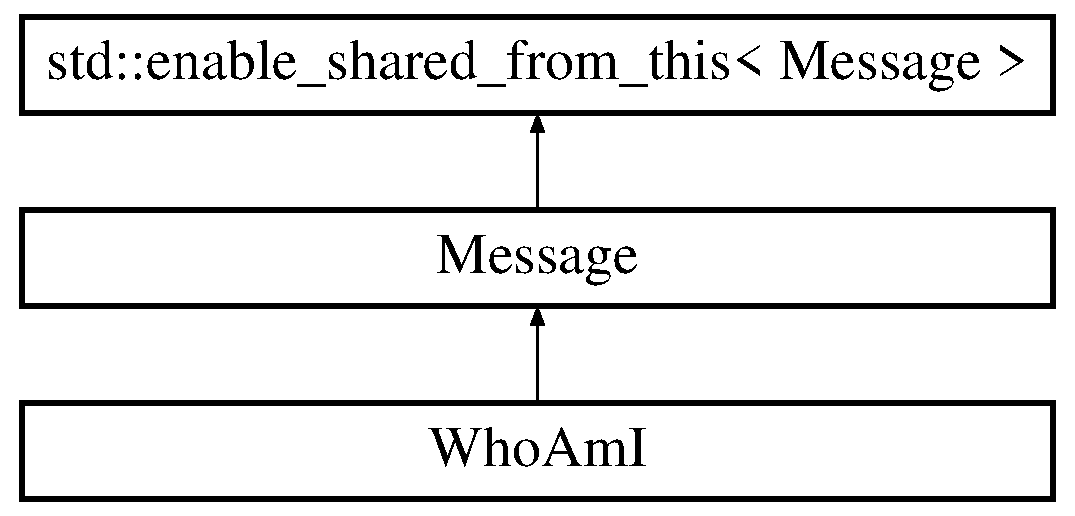
\includegraphics[height=3.000000cm]{classWhoAmI}
\end{center}
\end{figure}
\subsection*{Public Member Functions}
\begin{DoxyCompactItemize}
\item 
\mbox{\hyperlink{classWhoAmI_ae41a2e70254eb102102cd123d26b6c9f}{Who\+AmI}} ()
\item 
\mbox{\hyperlink{classWhoAmI_aa6d2d42633a1fd76e4aa76442f39c29a}{Who\+AmI}} (rapidjson\+::\+Document $\ast$doc)
\item 
rapidjson\+::\+Value \mbox{\hyperlink{classWhoAmI_a998c4b21d6235a84f15bd994b76be59d}{json}} (rapidjson\+::\+Document $\ast$document) const override
\end{DoxyCompactItemize}
\subsection*{Private Attributes}
\begin{DoxyCompactItemize}
\item 
int \mbox{\hyperlink{classWhoAmI_a5438cc57146d05f4f6b4fdfc155316fc}{version}}
\end{DoxyCompactItemize}
\subsection*{Additional Inherited Members}


\subsection{Constructor \& Destructor Documentation}
\mbox{\Hypertarget{classWhoAmI_ae41a2e70254eb102102cd123d26b6c9f}\label{classWhoAmI_ae41a2e70254eb102102cd123d26b6c9f}} 
\index{Who\+AmI@{Who\+AmI}!Who\+AmI@{Who\+AmI}}
\index{Who\+AmI@{Who\+AmI}!Who\+AmI@{Who\+AmI}}
\subsubsection{\texorpdfstring{Who\+Am\+I()}{WhoAmI()}\hspace{0.1cm}{\footnotesize\ttfamily [1/2]}}
{\footnotesize\ttfamily Who\+Am\+I\+::\+Who\+AmI (\begin{DoxyParamCaption}{ }\end{DoxyParamCaption})}

\mbox{\Hypertarget{classWhoAmI_aa6d2d42633a1fd76e4aa76442f39c29a}\label{classWhoAmI_aa6d2d42633a1fd76e4aa76442f39c29a}} 
\index{Who\+AmI@{Who\+AmI}!Who\+AmI@{Who\+AmI}}
\index{Who\+AmI@{Who\+AmI}!Who\+AmI@{Who\+AmI}}
\subsubsection{\texorpdfstring{Who\+Am\+I()}{WhoAmI()}\hspace{0.1cm}{\footnotesize\ttfamily [2/2]}}
{\footnotesize\ttfamily Who\+Am\+I\+::\+Who\+AmI (\begin{DoxyParamCaption}\item[{rapidjson\+::\+Document $\ast$}]{doc }\end{DoxyParamCaption})\hspace{0.3cm}{\ttfamily [explicit]}}



\subsection{Member Function Documentation}
\mbox{\Hypertarget{classWhoAmI_a998c4b21d6235a84f15bd994b76be59d}\label{classWhoAmI_a998c4b21d6235a84f15bd994b76be59d}} 
\index{Who\+AmI@{Who\+AmI}!json@{json}}
\index{json@{json}!Who\+AmI@{Who\+AmI}}
\subsubsection{\texorpdfstring{json()}{json()}}
{\footnotesize\ttfamily Value Who\+Am\+I\+::json (\begin{DoxyParamCaption}\item[{rapidjson\+::\+Document $\ast$}]{document }\end{DoxyParamCaption}) const\hspace{0.3cm}{\ttfamily [override]}, {\ttfamily [virtual]}}



Reimplemented from \mbox{\hyperlink{classMessage_a6f8e3ac2eed3a8afe9400fcd5b3447b2}{Message}}.



\subsection{Member Data Documentation}
\mbox{\Hypertarget{classWhoAmI_a5438cc57146d05f4f6b4fdfc155316fc}\label{classWhoAmI_a5438cc57146d05f4f6b4fdfc155316fc}} 
\index{Who\+AmI@{Who\+AmI}!version@{version}}
\index{version@{version}!Who\+AmI@{Who\+AmI}}
\subsubsection{\texorpdfstring{version}{version}}
{\footnotesize\ttfamily int Who\+Am\+I\+::version\hspace{0.3cm}{\ttfamily [private]}}



The documentation for this class was generated from the following files\+:\begin{DoxyCompactItemize}
\item 
include/\mbox{\hyperlink{messages_8hpp}{messages.\+hpp}}\item 
src/message/\mbox{\hyperlink{whoami_8cpp}{whoami.\+cpp}}\end{DoxyCompactItemize}

\chapter{File Documentation}
\hypertarget{blockchain_8hpp}{}\section{include/blockchain.hpp File Reference}
\label{blockchain_8hpp}\index{include/blockchain.\+hpp@{include/blockchain.\+hpp}}
{\ttfamily \#include \char`\"{}blocks.\+hpp\char`\"{}}\newline
{\ttfamily \#include $<$leveldb/db.\+h$>$}\newline
{\ttfamily \#include $<$string$>$}\newline
\subsection*{Classes}
\begin{DoxyCompactItemize}
\item 
class \mbox{\hyperlink{classBlockchain}{Blockchain}}
\end{DoxyCompactItemize}

\hypertarget{blocks_8hpp}{}\section{include/blocks.hpp File Reference}
\label{blocks_8hpp}\index{include/blocks.\+hpp@{include/blocks.\+hpp}}
{\ttfamily \#include $<$string$>$}\newline
{\ttfamily \#include $<$vector$>$}\newline
{\ttfamily \#include $<$memory$>$}\newline
{\ttfamily \#include $<$ctime$>$}\newline
{\ttfamily \#include $<$rapidjson/document.\+h$>$}\newline
{\ttfamily \#include \char`\"{}transaction.\+hpp\char`\"{}}\newline
{\ttfamily \#include \char`\"{}hashmemory.\+hpp\char`\"{}}\newline
\subsection*{Classes}
\begin{DoxyCompactItemize}
\item 
struct \mbox{\hyperlink{structBlockHeader}{Block\+Header}}
\begin{DoxyCompactList}\small\item\em Header of a \mbox{\hyperlink{classBlock}{Block}}. \end{DoxyCompactList}\item 
class \mbox{\hyperlink{classBlock}{Block}}
\begin{DoxyCompactList}\small\item\em \mbox{\hyperlink{classBlock}{Block}} of ensicoin \mbox{\hyperlink{classTransaction}{Transaction}}. \end{DoxyCompactList}\end{DoxyCompactItemize}

\hypertarget{connection_8hpp}{}\section{include/connection.hpp File Reference}
\label{connection_8hpp}\index{include/connection.\+hpp@{include/connection.\+hpp}}
{\ttfamily \#include \char`\"{}messages.\+hpp\char`\"{}}\newline
{\ttfamily \#include $<$asio.\+hpp$>$}\newline
{\ttfamily \#include $<$memory$>$}\newline
{\ttfamily \#include $<$rapidjson/document.\+h$>$}\newline
\subsection*{Classes}
\begin{DoxyCompactItemize}
\item 
class \mbox{\hyperlink{classConnection}{Connection}}
\begin{DoxyCompactList}\small\item\em A \mbox{\hyperlink{classConnection}{Connection}} to a peer. \end{DoxyCompactList}\end{DoxyCompactItemize}

\hypertarget{constants_8hpp}{}\section{include/constants.hpp File Reference}
\label{constants_8hpp}\index{include/constants.\+hpp@{include/constants.\+hpp}}
{\ttfamily \#include $<$cstdlib$>$}\newline
{\ttfamily \#include $<$string$>$}\newline
\subsection*{Variables}
\begin{DoxyCompactItemize}
\item 
constexpr int \mbox{\hyperlink{constants_8hpp_ab3abf628bb70723a3fa493968117815b}{M\+A\+X\+\_\+\+B\+L\+O\+C\+K\+\_\+\+S\+I\+ZE}} = 2$\ast$1024
\begin{DoxyCompactList}\small\item\em Maximum size of a \mbox{\hyperlink{classBlock}{Block}}. \end{DoxyCompactList}\item 
constexpr int \mbox{\hyperlink{constants_8hpp_aa83d2186d4c042afdbcb997b8525e493}{M\+E\+S\+S\+A\+G\+E\+\_\+\+L\+I\+M\+IT}} = 2$\ast$\mbox{\hyperlink{constants_8hpp_ab3abf628bb70723a3fa493968117815b}{M\+A\+X\+\_\+\+B\+L\+O\+C\+K\+\_\+\+S\+I\+ZE}}
\begin{DoxyCompactList}\small\item\em Maximum number of characters in a \mbox{\hyperlink{classMessage}{Message}}. \end{DoxyCompactList}\item 
constexpr int \mbox{\hyperlink{constants_8hpp_a2b4d9172503c0e7acc008c8064e7a759}{V\+E\+R\+S\+I\+ON}} = 0
\begin{DoxyCompactList}\small\item\em Protocol version. \end{DoxyCompactList}\item 
constexpr int \mbox{\hyperlink{constants_8hpp_aec426389714e5cfff7d295211c805dc0}{M\+A\+G\+IC}} = 422021
\begin{DoxyCompactList}\small\item\em Magic number of the network. \end{DoxyCompactList}\item 
constexpr int \mbox{\hyperlink{constants_8hpp_a765a3ccfceadb6670202a0753b6f61f1}{P\+O\+RT}} = 4224
\begin{DoxyCompactList}\small\item\em Port used on the network. \end{DoxyCompactList}\item 
const std\+::string \mbox{\hyperlink{constants_8hpp_adc448fae121fe6b350fa3034e3948d3e}{D\+A\+T\+A\+\_\+\+P\+A\+TH}}
\begin{DoxyCompactList}\small\item\em Path to application data. \end{DoxyCompactList}\item 
const std\+::string \mbox{\hyperlink{constants_8hpp_a569fba83b3e13903d421745af52aac12}{U\+T\+X\+O\+\_\+\+DB}}
\begin{DoxyCompactList}\small\item\em folder of U\+T\+XO database \end{DoxyCompactList}\item 
const std\+::string \mbox{\hyperlink{constants_8hpp_a3d7a816927147968e177bbd8092bc864}{B\+L\+O\+C\+K\+C\+H\+A\+I\+N\+\_\+\+DB}}
\begin{DoxyCompactList}\small\item\em folder of \mbox{\hyperlink{classBlockchain}{Blockchain}} database \end{DoxyCompactList}\end{DoxyCompactItemize}


\subsection{Variable Documentation}
\mbox{\Hypertarget{constants_8hpp_a3d7a816927147968e177bbd8092bc864}\label{constants_8hpp_a3d7a816927147968e177bbd8092bc864}} 
\index{constants.\+hpp@{constants.\+hpp}!B\+L\+O\+C\+K\+C\+H\+A\+I\+N\+\_\+\+DB@{B\+L\+O\+C\+K\+C\+H\+A\+I\+N\+\_\+\+DB}}
\index{B\+L\+O\+C\+K\+C\+H\+A\+I\+N\+\_\+\+DB@{B\+L\+O\+C\+K\+C\+H\+A\+I\+N\+\_\+\+DB}!constants.\+hpp@{constants.\+hpp}}
\subsubsection{\texorpdfstring{B\+L\+O\+C\+K\+C\+H\+A\+I\+N\+\_\+\+DB}{BLOCKCHAIN\_DB}}
{\footnotesize\ttfamily const std\+::string B\+L\+O\+C\+K\+C\+H\+A\+I\+N\+\_\+\+DB}



folder of \mbox{\hyperlink{classBlockchain}{Blockchain}} database 

\mbox{\Hypertarget{constants_8hpp_adc448fae121fe6b350fa3034e3948d3e}\label{constants_8hpp_adc448fae121fe6b350fa3034e3948d3e}} 
\index{constants.\+hpp@{constants.\+hpp}!D\+A\+T\+A\+\_\+\+P\+A\+TH@{D\+A\+T\+A\+\_\+\+P\+A\+TH}}
\index{D\+A\+T\+A\+\_\+\+P\+A\+TH@{D\+A\+T\+A\+\_\+\+P\+A\+TH}!constants.\+hpp@{constants.\+hpp}}
\subsubsection{\texorpdfstring{D\+A\+T\+A\+\_\+\+P\+A\+TH}{DATA\_PATH}}
{\footnotesize\ttfamily const std\+::string D\+A\+T\+A\+\_\+\+P\+A\+TH}



Path to application data. 

\mbox{\Hypertarget{constants_8hpp_aec426389714e5cfff7d295211c805dc0}\label{constants_8hpp_aec426389714e5cfff7d295211c805dc0}} 
\index{constants.\+hpp@{constants.\+hpp}!M\+A\+G\+IC@{M\+A\+G\+IC}}
\index{M\+A\+G\+IC@{M\+A\+G\+IC}!constants.\+hpp@{constants.\+hpp}}
\subsubsection{\texorpdfstring{M\+A\+G\+IC}{MAGIC}}
{\footnotesize\ttfamily constexpr int M\+A\+G\+IC = 422021}



Magic number of the network. 

\mbox{\Hypertarget{constants_8hpp_ab3abf628bb70723a3fa493968117815b}\label{constants_8hpp_ab3abf628bb70723a3fa493968117815b}} 
\index{constants.\+hpp@{constants.\+hpp}!M\+A\+X\+\_\+\+B\+L\+O\+C\+K\+\_\+\+S\+I\+ZE@{M\+A\+X\+\_\+\+B\+L\+O\+C\+K\+\_\+\+S\+I\+ZE}}
\index{M\+A\+X\+\_\+\+B\+L\+O\+C\+K\+\_\+\+S\+I\+ZE@{M\+A\+X\+\_\+\+B\+L\+O\+C\+K\+\_\+\+S\+I\+ZE}!constants.\+hpp@{constants.\+hpp}}
\subsubsection{\texorpdfstring{M\+A\+X\+\_\+\+B\+L\+O\+C\+K\+\_\+\+S\+I\+ZE}{MAX\_BLOCK\_SIZE}}
{\footnotesize\ttfamily constexpr int M\+A\+X\+\_\+\+B\+L\+O\+C\+K\+\_\+\+S\+I\+ZE = 2$\ast$1024}



Maximum size of a \mbox{\hyperlink{classBlock}{Block}}. 

\mbox{\Hypertarget{constants_8hpp_aa83d2186d4c042afdbcb997b8525e493}\label{constants_8hpp_aa83d2186d4c042afdbcb997b8525e493}} 
\index{constants.\+hpp@{constants.\+hpp}!M\+E\+S\+S\+A\+G\+E\+\_\+\+L\+I\+M\+IT@{M\+E\+S\+S\+A\+G\+E\+\_\+\+L\+I\+M\+IT}}
\index{M\+E\+S\+S\+A\+G\+E\+\_\+\+L\+I\+M\+IT@{M\+E\+S\+S\+A\+G\+E\+\_\+\+L\+I\+M\+IT}!constants.\+hpp@{constants.\+hpp}}
\subsubsection{\texorpdfstring{M\+E\+S\+S\+A\+G\+E\+\_\+\+L\+I\+M\+IT}{MESSAGE\_LIMIT}}
{\footnotesize\ttfamily constexpr int M\+E\+S\+S\+A\+G\+E\+\_\+\+L\+I\+M\+IT = 2$\ast$\mbox{\hyperlink{constants_8hpp_ab3abf628bb70723a3fa493968117815b}{M\+A\+X\+\_\+\+B\+L\+O\+C\+K\+\_\+\+S\+I\+ZE}}}



Maximum number of characters in a \mbox{\hyperlink{classMessage}{Message}}. 

\mbox{\Hypertarget{constants_8hpp_a765a3ccfceadb6670202a0753b6f61f1}\label{constants_8hpp_a765a3ccfceadb6670202a0753b6f61f1}} 
\index{constants.\+hpp@{constants.\+hpp}!P\+O\+RT@{P\+O\+RT}}
\index{P\+O\+RT@{P\+O\+RT}!constants.\+hpp@{constants.\+hpp}}
\subsubsection{\texorpdfstring{P\+O\+RT}{PORT}}
{\footnotesize\ttfamily constexpr int P\+O\+RT = 4224}



Port used on the network. 

\mbox{\Hypertarget{constants_8hpp_a569fba83b3e13903d421745af52aac12}\label{constants_8hpp_a569fba83b3e13903d421745af52aac12}} 
\index{constants.\+hpp@{constants.\+hpp}!U\+T\+X\+O\+\_\+\+DB@{U\+T\+X\+O\+\_\+\+DB}}
\index{U\+T\+X\+O\+\_\+\+DB@{U\+T\+X\+O\+\_\+\+DB}!constants.\+hpp@{constants.\+hpp}}
\subsubsection{\texorpdfstring{U\+T\+X\+O\+\_\+\+DB}{UTXO\_DB}}
{\footnotesize\ttfamily const std\+::string U\+T\+X\+O\+\_\+\+DB}



folder of U\+T\+XO database 

\mbox{\Hypertarget{constants_8hpp_a2b4d9172503c0e7acc008c8064e7a759}\label{constants_8hpp_a2b4d9172503c0e7acc008c8064e7a759}} 
\index{constants.\+hpp@{constants.\+hpp}!V\+E\+R\+S\+I\+ON@{V\+E\+R\+S\+I\+ON}}
\index{V\+E\+R\+S\+I\+ON@{V\+E\+R\+S\+I\+ON}!constants.\+hpp@{constants.\+hpp}}
\subsubsection{\texorpdfstring{V\+E\+R\+S\+I\+ON}{VERSION}}
{\footnotesize\ttfamily constexpr int V\+E\+R\+S\+I\+ON = 0}



Protocol version. 


\hypertarget{crypto_8hpp}{}\section{include/crypto.hpp File Reference}
\label{crypto_8hpp}\index{include/crypto.\+hpp@{include/crypto.\+hpp}}
{\ttfamily \#include $<$string$>$}\newline
{\ttfamily \#include $<$memory$>$}\newline
{\ttfamily \#include $<$cryptopp/integer.\+h$>$}\newline
{\ttfamily \#include $<$cryptopp/eccrypto.\+h$>$}\newline
\subsection*{Classes}
\begin{DoxyCompactItemize}
\item 
class \mbox{\hyperlink{classECDSASignature}{E\+C\+D\+S\+A\+Signature}}
\begin{DoxyCompactList}\small\item\em Signatures using secp256k1. \end{DoxyCompactList}\end{DoxyCompactItemize}
\subsection*{Typedefs}
\begin{DoxyCompactItemize}
\item 
using \mbox{\hyperlink{crypto_8hpp_a23367062568b66a23ab6d441eb04c2d5}{e\+Curve}} = E\+C\+D\+SA$<$ E\+CP, S\+H\+A256 $>$
\end{DoxyCompactItemize}
\subsection*{Functions}
\begin{DoxyCompactItemize}
\item 
std\+::string \mbox{\hyperlink{crypto_8hpp_ac2f5f72ad1535f19f85ac0d91c896e6c}{ripemd160}} (std\+::string input, bool unpack=false)
\begin{DoxyCompactList}\small\item\em Take the R\+I\+P\+E\+M\+D160 hash. \end{DoxyCompactList}\item 
std\+::string \mbox{\hyperlink{crypto_8hpp_a6ba01f11a1b2f987950b2909a08fef50}{sha256}} (std\+::string input, bool unpack=false)
\begin{DoxyCompactList}\small\item\em Take the S\+H\+A256 hash. \end{DoxyCompactList}\item 
std\+::string \mbox{\hyperlink{crypto_8hpp_a38fe04188a987a4105b1b2f4264e568b}{hex\+Public\+Key}} (const E\+C\+P\+::\+Point q)
\begin{DoxyCompactList}\small\item\em Hex reprensation of a public key. \end{DoxyCompactList}\end{DoxyCompactItemize}


\subsection{Typedef Documentation}
\mbox{\Hypertarget{crypto_8hpp_a23367062568b66a23ab6d441eb04c2d5}\label{crypto_8hpp_a23367062568b66a23ab6d441eb04c2d5}} 
\index{crypto.\+hpp@{crypto.\+hpp}!e\+Curve@{e\+Curve}}
\index{e\+Curve@{e\+Curve}!crypto.\+hpp@{crypto.\+hpp}}
\subsubsection{\texorpdfstring{e\+Curve}{eCurve}}
{\footnotesize\ttfamily using \mbox{\hyperlink{crypto_8hpp_a23367062568b66a23ab6d441eb04c2d5}{e\+Curve}} =  E\+C\+D\+SA$<$E\+CP, S\+H\+A256$>$}



\subsection{Function Documentation}
\mbox{\Hypertarget{crypto_8hpp_a38fe04188a987a4105b1b2f4264e568b}\label{crypto_8hpp_a38fe04188a987a4105b1b2f4264e568b}} 
\index{crypto.\+hpp@{crypto.\+hpp}!hex\+Public\+Key@{hex\+Public\+Key}}
\index{hex\+Public\+Key@{hex\+Public\+Key}!crypto.\+hpp@{crypto.\+hpp}}
\subsubsection{\texorpdfstring{hex\+Public\+Key()}{hexPublicKey()}}
{\footnotesize\ttfamily std\+::string hex\+Public\+Key (\begin{DoxyParamCaption}\item[{const E\+C\+P\+::\+Point}]{q }\end{DoxyParamCaption})}



Hex reprensation of a public key. 

q public point on secp256k1 \mbox{\Hypertarget{crypto_8hpp_ac2f5f72ad1535f19f85ac0d91c896e6c}\label{crypto_8hpp_ac2f5f72ad1535f19f85ac0d91c896e6c}} 
\index{crypto.\+hpp@{crypto.\+hpp}!ripemd160@{ripemd160}}
\index{ripemd160@{ripemd160}!crypto.\+hpp@{crypto.\+hpp}}
\subsubsection{\texorpdfstring{ripemd160()}{ripemd160()}}
{\footnotesize\ttfamily std\+::string ripemd160 (\begin{DoxyParamCaption}\item[{std\+::string}]{input,  }\item[{bool}]{unpack = {\ttfamily false} }\end{DoxyParamCaption})}



Take the R\+I\+P\+E\+M\+D160 hash. 


\begin{DoxyParams}{Parameters}
{\em input} & string to be hashed \\
\hline
{\em unpack} & handles a binary string \\
\hline
\end{DoxyParams}
\mbox{\Hypertarget{crypto_8hpp_a6ba01f11a1b2f987950b2909a08fef50}\label{crypto_8hpp_a6ba01f11a1b2f987950b2909a08fef50}} 
\index{crypto.\+hpp@{crypto.\+hpp}!sha256@{sha256}}
\index{sha256@{sha256}!crypto.\+hpp@{crypto.\+hpp}}
\subsubsection{\texorpdfstring{sha256()}{sha256()}}
{\footnotesize\ttfamily std\+::string sha256 (\begin{DoxyParamCaption}\item[{std\+::string}]{input,  }\item[{bool}]{unpack = {\ttfamily false} }\end{DoxyParamCaption})}



Take the S\+H\+A256 hash. 


\begin{DoxyParams}{Parameters}
{\em input} & string to be hashed \\
\hline
{\em unpack} & handles a binary string \\
\hline
\end{DoxyParams}

\hypertarget{hashmemory_8hpp}{}\section{include/hashmemory.hpp File Reference}
\label{hashmemory_8hpp}\index{include/hashmemory.\+hpp@{include/hashmemory.\+hpp}}
{\ttfamily \#include $<$unordered\+\_\+map$>$}\newline
{\ttfamily \#include $<$memory$>$}\newline
{\ttfamily \#include $<$string$>$}\newline
\subsection*{Classes}
\begin{DoxyCompactItemize}
\item 
class \mbox{\hyperlink{classHashMemory}{Hash\+Memory$<$ T $>$}}
\begin{DoxyCompactList}\small\item\em Wrapper around a std\+::unordered\+\_\+map. \end{DoxyCompactList}\end{DoxyCompactItemize}

\hypertarget{mempool_8hpp}{}\section{include/mempool.hpp File Reference}
\label{mempool_8hpp}\index{include/mempool.\+hpp@{include/mempool.\+hpp}}
{\ttfamily \#include \char`\"{}hashmemory.\+hpp\char`\"{}}\newline
{\ttfamily \#include \char`\"{}transaction.\+hpp\char`\"{}}\newline
{\ttfamily \#include \char`\"{}utxo.\+hpp\char`\"{}}\newline
{\ttfamily \#include $<$map$>$}\newline
{\ttfamily \#include $<$memory$>$}\newline
{\ttfamily \#include $<$string$>$}\newline
{\ttfamily \#include $<$vector$>$}\newline
\subsection*{Classes}
\begin{DoxyCompactItemize}
\item 
class \mbox{\hyperlink{classMempool}{Mempool}}
\begin{DoxyCompactList}\small\item\em Pool of \mbox{\hyperlink{classTransaction}{Transaction}} not in \mbox{\hyperlink{classBlock}{Block}}. \end{DoxyCompactList}\end{DoxyCompactItemize}

\hypertarget{messagehandler_8hpp}{}\section{include/messagehandler.hpp File Reference}
\label{messagehandler_8hpp}\index{include/messagehandler.\+hpp@{include/messagehandler.\+hpp}}
{\ttfamily \#include $<$memory$>$}\newline
{\ttfamily \#include \char`\"{}messages.\+hpp\char`\"{}}\newline
\subsection*{Classes}
\begin{DoxyCompactItemize}
\item 
class \mbox{\hyperlink{classHandler}{Handler}}
\item 
struct \mbox{\hyperlink{structHandler_1_1params}{Handler\+::params}}
\end{DoxyCompactItemize}

\hypertarget{messages_8hpp}{}\section{include/messages.hpp File Reference}
\label{messages_8hpp}\index{include/messages.\+hpp@{include/messages.\+hpp}}
{\ttfamily \#include \char`\"{}blocks.\+hpp\char`\"{}}\newline
{\ttfamily \#include \char`\"{}transaction.\+hpp\char`\"{}}\newline
{\ttfamily \#include $<$ctime$>$}\newline
{\ttfamily \#include $<$memory$>$}\newline
{\ttfamily \#include $<$rapidjson/document.\+h$>$}\newline
{\ttfamily \#include $<$string$>$}\newline
{\ttfamily \#include $<$vector$>$}\newline
\subsection*{Classes}
\begin{DoxyCompactItemize}
\item 
class \mbox{\hyperlink{classMessage}{Message}}
\item 
class \mbox{\hyperlink{classWhoAmI}{Who\+AmI}}
\item 
struct \mbox{\hyperlink{structInvData}{Inv\+Data}}
\item 
class \mbox{\hyperlink{classInv}{Inv}}
\item 
class \mbox{\hyperlink{classGetData}{Get\+Data}}
\item 
class \mbox{\hyperlink{classNotFound}{Not\+Found}}
\item 
class \mbox{\hyperlink{classBlockMessage}{Block\+Message}}
\item 
class \mbox{\hyperlink{classTransactionMessage}{Transaction\+Message}}
\item 
class \mbox{\hyperlink{classGetBlocks}{Get\+Blocks}}
\item 
class \mbox{\hyperlink{classGetMempool}{Get\+Mempool}}
\end{DoxyCompactItemize}

\hypertarget{node_8hpp}{}\section{include/node.hpp File Reference}
\label{node_8hpp}\index{include/node.\+hpp@{include/node.\+hpp}}
{\ttfamily \#include \char`\"{}blockchain.\+hpp\char`\"{}}\newline
{\ttfamily \#include \char`\"{}blocks.\+hpp\char`\"{}}\newline
{\ttfamily \#include \char`\"{}connection.\+hpp\char`\"{}}\newline
{\ttfamily \#include \char`\"{}hashmemory.\+hpp\char`\"{}}\newline
{\ttfamily \#include \char`\"{}mempool.\+hpp\char`\"{}}\newline
{\ttfamily \#include \char`\"{}transaction.\+hpp\char`\"{}}\newline
{\ttfamily \#include \char`\"{}utxo.\+hpp\char`\"{}}\newline
{\ttfamily \#include $<$asio.\+hpp$>$}\newline
{\ttfamily \#include $<$memory$>$}\newline
{\ttfamily \#include $<$vector$>$}\newline
\subsection*{Classes}
\begin{DoxyCompactItemize}
\item 
class \mbox{\hyperlink{classNode}{Node}}
\begin{DoxyCompactList}\small\item\em \mbox{\hyperlink{classNode}{Node}} handling messages and processing. \end{DoxyCompactList}\end{DoxyCompactItemize}

\hypertarget{script_8hpp}{}\section{include/script.hpp File Reference}
\label{script_8hpp}\index{include/script.\+hpp@{include/script.\+hpp}}
{\ttfamily \#include $<$string$>$}\newline
{\ttfamily \#include $<$vector$>$}\newline
{\ttfamily \#include $<$iterator$>$}\newline
{\ttfamily \#include $<$stack$>$}\newline
\subsection*{Classes}
\begin{DoxyCompactItemize}
\item 
class \mbox{\hyperlink{classScript}{Script}}
\end{DoxyCompactItemize}

\hypertarget{transaction_8hpp}{}\section{include/transaction.hpp File Reference}
\label{transaction_8hpp}\index{include/transaction.\+hpp@{include/transaction.\+hpp}}
{\ttfamily \#include \char`\"{}hashmemory.\+hpp\char`\"{}}\newline
{\ttfamily \#include \char`\"{}script.\+hpp\char`\"{}}\newline
{\ttfamily \#include $<$iterator$>$}\newline
{\ttfamily \#include $<$memory$>$}\newline
{\ttfamily \#include $<$rapidjson/document.\+h$>$}\newline
{\ttfamily \#include $<$sstream$>$}\newline
{\ttfamily \#include $<$stack$>$}\newline
{\ttfamily \#include $<$string$>$}\newline
{\ttfamily \#include $<$vector$>$}\newline
\subsection*{Classes}
\begin{DoxyCompactItemize}
\item 
struct \mbox{\hyperlink{structTransactionIdentifier}{Transaction\+Identifier}}
\item 
struct \mbox{\hyperlink{structInputTransaction}{Input\+Transaction}}
\item 
struct \mbox{\hyperlink{structOutputTransaction}{Output\+Transaction}}
\item 
class \mbox{\hyperlink{classTransaction}{Transaction}}
\end{DoxyCompactItemize}
\subsection*{Enumerations}
\begin{DoxyCompactItemize}
\item 
enum \mbox{\hyperlink{transaction_8hpp_a379269e60c4ed3fb09a01778f31ddaad}{T\+X\+Type}} \{ \mbox{\hyperlink{transaction_8hpp_a379269e60c4ed3fb09a01778f31ddaada134347527140a1931e0d675afc6cafa3}{Orphan}}, 
\mbox{\hyperlink{transaction_8hpp_a379269e60c4ed3fb09a01778f31ddaada66dfad2fc66aab9e6bb47cfad78b4b6b}{Regular}}
 \}
\end{DoxyCompactItemize}


\subsection{Enumeration Type Documentation}
\mbox{\Hypertarget{transaction_8hpp_a379269e60c4ed3fb09a01778f31ddaad}\label{transaction_8hpp_a379269e60c4ed3fb09a01778f31ddaad}} 
\index{transaction.\+hpp@{transaction.\+hpp}!T\+X\+Type@{T\+X\+Type}}
\index{T\+X\+Type@{T\+X\+Type}!transaction.\+hpp@{transaction.\+hpp}}
\subsubsection{\texorpdfstring{T\+X\+Type}{TXType}}
{\footnotesize\ttfamily enum \mbox{\hyperlink{transaction_8hpp_a379269e60c4ed3fb09a01778f31ddaad}{T\+X\+Type}}}

\begin{DoxyEnumFields}{Enumerator}
\raisebox{\heightof{T}}[0pt][0pt]{\index{Orphan@{Orphan}!transaction.\+hpp@{transaction.\+hpp}}\index{transaction.\+hpp@{transaction.\+hpp}!Orphan@{Orphan}}}\mbox{\Hypertarget{transaction_8hpp_a379269e60c4ed3fb09a01778f31ddaada134347527140a1931e0d675afc6cafa3}\label{transaction_8hpp_a379269e60c4ed3fb09a01778f31ddaada134347527140a1931e0d675afc6cafa3}} 
Orphan&\\
\hline

\raisebox{\heightof{T}}[0pt][0pt]{\index{Regular@{Regular}!transaction.\+hpp@{transaction.\+hpp}}\index{transaction.\+hpp@{transaction.\+hpp}!Regular@{Regular}}}\mbox{\Hypertarget{transaction_8hpp_a379269e60c4ed3fb09a01778f31ddaada66dfad2fc66aab9e6bb47cfad78b4b6b}\label{transaction_8hpp_a379269e60c4ed3fb09a01778f31ddaada66dfad2fc66aab9e6bb47cfad78b4b6b}} 
Regular&\\
\hline

\end{DoxyEnumFields}

\hypertarget{utxo_8hpp}{}\section{include/utxo.hpp File Reference}
\label{utxo_8hpp}\index{include/utxo.\+hpp@{include/utxo.\+hpp}}
{\ttfamily \#include \char`\"{}transaction.\+hpp\char`\"{}}\newline
{\ttfamily \#include $<$leveldb/db.\+h$>$}\newline
{\ttfamily \#include $<$memory$>$}\newline
{\ttfamily \#include $<$string$>$}\newline
\subsection*{Classes}
\begin{DoxyCompactItemize}
\item 
struct \mbox{\hyperlink{structUTXOdata}{U\+T\+X\+Odata}}
\item 
class \mbox{\hyperlink{classUTXOManager}{U\+T\+X\+O\+Manager}}
\end{DoxyCompactItemize}
\subsection*{Typedefs}
\begin{DoxyCompactItemize}
\item 
using \mbox{\hyperlink{utxo_8hpp_a19091d002da03ec92277e19295ac4540}{U\+T\+XO}} = \mbox{\hyperlink{structTransactionIdentifier}{Transaction\+Identifier}}
\end{DoxyCompactItemize}


\subsection{Typedef Documentation}
\mbox{\Hypertarget{utxo_8hpp_a19091d002da03ec92277e19295ac4540}\label{utxo_8hpp_a19091d002da03ec92277e19295ac4540}} 
\index{utxo.\+hpp@{utxo.\+hpp}!U\+T\+XO@{U\+T\+XO}}
\index{U\+T\+XO@{U\+T\+XO}!utxo.\+hpp@{utxo.\+hpp}}
\subsubsection{\texorpdfstring{U\+T\+XO}{UTXO}}
{\footnotesize\ttfamily using \mbox{\hyperlink{utxo_8hpp_a19091d002da03ec92277e19295ac4540}{U\+T\+XO}} =  \mbox{\hyperlink{structTransactionIdentifier}{Transaction\+Identifier}}}


\hypertarget{README_8md}{}\section{R\+E\+A\+D\+M\+E.\+md File Reference}
\label{README_8md}\index{R\+E\+A\+D\+M\+E.\+md@{R\+E\+A\+D\+M\+E.\+md}}

\hypertarget{blockchain_8cpp}{}\section{src/blockchain.cpp File Reference}
\label{blockchain_8cpp}\index{src/blockchain.\+cpp@{src/blockchain.\+cpp}}
{\ttfamily \#include \char`\"{}blockchain.\+hpp\char`\"{}}\newline
{\ttfamily \#include \char`\"{}constants.\+hpp\char`\"{}}\newline
{\ttfamily \#include $<$iostream$>$}\newline
{\ttfamily \#include $<$leveldb/db.\+h$>$}\newline

\hypertarget{blocks_8cpp}{}\section{src/blocks.cpp File Reference}
\label{blocks_8cpp}\index{src/blocks.\+cpp@{src/blocks.\+cpp}}
{\ttfamily \#include \char`\"{}blocks.\+hpp\char`\"{}}\newline
{\ttfamily \#include \char`\"{}crypto.\+hpp\char`\"{}}\newline
{\ttfamily \#include \char`\"{}transaction.\+hpp\char`\"{}}\newline
{\ttfamily \#include $<$rapidjson/document.\+h$>$}\newline
{\ttfamily \#include $<$vector$>$}\newline
{\ttfamily \#include $<$string$>$}\newline
{\ttfamily \#include $<$memory$>$}\newline
{\ttfamily \#include $<$sstream$>$}\newline

\hypertarget{connection_8cpp}{}\section{src/connection.cpp File Reference}
\label{connection_8cpp}\index{src/connection.\+cpp@{src/connection.\+cpp}}
{\ttfamily \#include \char`\"{}connection.\+hpp\char`\"{}}\newline
{\ttfamily \#include \char`\"{}constants.\+hpp\char`\"{}}\newline
{\ttfamily \#include \char`\"{}messagehandler.\+hpp\char`\"{}}\newline
{\ttfamily \#include \char`\"{}messages.\+hpp\char`\"{}}\newline
{\ttfamily \#include $<$asio.\+hpp$>$}\newline
{\ttfamily \#include $<$cstring$>$}\newline
{\ttfamily \#include $<$functional$>$}\newline
{\ttfamily \#include $<$iostream$>$}\newline
{\ttfamily \#include $<$memory$>$}\newline
{\ttfamily \#include $<$rapidjson/document.\+h$>$}\newline
{\ttfamily \#include $<$stdexcept$>$}\newline

\hypertarget{constants_8cpp}{}\section{src/constants.cpp File Reference}
\label{constants_8cpp}\index{src/constants.\+cpp@{src/constants.\+cpp}}
{\ttfamily \#include \char`\"{}constants.\+hpp\char`\"{}}\newline
{\ttfamily \#include $<$cstdlib$>$}\newline
{\ttfamily \#include $<$string$>$}\newline
\subsection*{Variables}
\begin{DoxyCompactItemize}
\item 
const std\+::string \mbox{\hyperlink{constants_8cpp_adc448fae121fe6b350fa3034e3948d3e}{D\+A\+T\+A\+\_\+\+P\+A\+TH}} = std\+::string(std\+::getenv(\char`\"{}H\+O\+ME\char`\"{})) + \char`\"{}/.ensicoincpp\char`\"{}
\begin{DoxyCompactList}\small\item\em Path to application data. \end{DoxyCompactList}\item 
const std\+::string \mbox{\hyperlink{constants_8cpp_a569fba83b3e13903d421745af52aac12}{U\+T\+X\+O\+\_\+\+DB}} = \mbox{\hyperlink{constants_8cpp_adc448fae121fe6b350fa3034e3948d3e}{D\+A\+T\+A\+\_\+\+P\+A\+TH}} + \char`\"{}/utxo\char`\"{}
\begin{DoxyCompactList}\small\item\em folder of U\+T\+XO database \end{DoxyCompactList}\item 
const std\+::string \mbox{\hyperlink{constants_8cpp_a3d7a816927147968e177bbd8092bc864}{B\+L\+O\+C\+K\+C\+H\+A\+I\+N\+\_\+\+DB}} = \mbox{\hyperlink{constants_8cpp_adc448fae121fe6b350fa3034e3948d3e}{D\+A\+T\+A\+\_\+\+P\+A\+TH}} + \char`\"{}/blockchain\char`\"{}
\begin{DoxyCompactList}\small\item\em folder of \mbox{\hyperlink{classBlockchain}{Blockchain}} database \end{DoxyCompactList}\end{DoxyCompactItemize}


\subsection{Variable Documentation}
\mbox{\Hypertarget{constants_8cpp_a3d7a816927147968e177bbd8092bc864}\label{constants_8cpp_a3d7a816927147968e177bbd8092bc864}} 
\index{constants.\+cpp@{constants.\+cpp}!B\+L\+O\+C\+K\+C\+H\+A\+I\+N\+\_\+\+DB@{B\+L\+O\+C\+K\+C\+H\+A\+I\+N\+\_\+\+DB}}
\index{B\+L\+O\+C\+K\+C\+H\+A\+I\+N\+\_\+\+DB@{B\+L\+O\+C\+K\+C\+H\+A\+I\+N\+\_\+\+DB}!constants.\+cpp@{constants.\+cpp}}
\subsubsection{\texorpdfstring{B\+L\+O\+C\+K\+C\+H\+A\+I\+N\+\_\+\+DB}{BLOCKCHAIN\_DB}}
{\footnotesize\ttfamily const std\+::string B\+L\+O\+C\+K\+C\+H\+A\+I\+N\+\_\+\+DB = \mbox{\hyperlink{constants_8cpp_adc448fae121fe6b350fa3034e3948d3e}{D\+A\+T\+A\+\_\+\+P\+A\+TH}} + \char`\"{}/blockchain\char`\"{}}



folder of \mbox{\hyperlink{classBlockchain}{Blockchain}} database 

\mbox{\Hypertarget{constants_8cpp_adc448fae121fe6b350fa3034e3948d3e}\label{constants_8cpp_adc448fae121fe6b350fa3034e3948d3e}} 
\index{constants.\+cpp@{constants.\+cpp}!D\+A\+T\+A\+\_\+\+P\+A\+TH@{D\+A\+T\+A\+\_\+\+P\+A\+TH}}
\index{D\+A\+T\+A\+\_\+\+P\+A\+TH@{D\+A\+T\+A\+\_\+\+P\+A\+TH}!constants.\+cpp@{constants.\+cpp}}
\subsubsection{\texorpdfstring{D\+A\+T\+A\+\_\+\+P\+A\+TH}{DATA\_PATH}}
{\footnotesize\ttfamily const std\+::string D\+A\+T\+A\+\_\+\+P\+A\+TH = std\+::string(std\+::getenv(\char`\"{}H\+O\+ME\char`\"{})) + \char`\"{}/.ensicoincpp\char`\"{}}



Path to application data. 

\mbox{\Hypertarget{constants_8cpp_a569fba83b3e13903d421745af52aac12}\label{constants_8cpp_a569fba83b3e13903d421745af52aac12}} 
\index{constants.\+cpp@{constants.\+cpp}!U\+T\+X\+O\+\_\+\+DB@{U\+T\+X\+O\+\_\+\+DB}}
\index{U\+T\+X\+O\+\_\+\+DB@{U\+T\+X\+O\+\_\+\+DB}!constants.\+cpp@{constants.\+cpp}}
\subsubsection{\texorpdfstring{U\+T\+X\+O\+\_\+\+DB}{UTXO\_DB}}
{\footnotesize\ttfamily const std\+::string U\+T\+X\+O\+\_\+\+DB = \mbox{\hyperlink{constants_8cpp_adc448fae121fe6b350fa3034e3948d3e}{D\+A\+T\+A\+\_\+\+P\+A\+TH}} + \char`\"{}/utxo\char`\"{}}



folder of U\+T\+XO database 


\hypertarget{crypto_8cpp}{}\section{src/crypto.cpp File Reference}
\label{crypto_8cpp}\index{src/crypto.\+cpp@{src/crypto.\+cpp}}
{\ttfamily \#include $<$iostream$>$}\newline
{\ttfamily \#include $<$sstream$>$}\newline
{\ttfamily \#include $<$string$>$}\newline
{\ttfamily \#include $<$cryptopp/eccrypto.\+h$>$}\newline
{\ttfamily \#include $<$cryptopp/ripemd.\+h$>$}\newline
{\ttfamily \#include $<$cryptopp/filters.\+h$>$}\newline
{\ttfamily \#include $<$cryptopp/hex.\+h$>$}\newline
{\ttfamily \#include $<$cryptopp/oids.\+h$>$}\newline
{\ttfamily \#include $<$cryptopp/osrng.\+h$>$}\newline
{\ttfamily \#include \char`\"{}crypto.\+hpp\char`\"{}}\newline
\subsection*{Functions}
\begin{DoxyCompactItemize}
\item 
std\+::string \mbox{\hyperlink{crypto_8cpp_a38fe04188a987a4105b1b2f4264e568b}{hex\+Public\+Key}} (const E\+C\+P\+::\+Point q)
\begin{DoxyCompactList}\small\item\em Hex reprensation of a public key. \end{DoxyCompactList}\item 
std\+::string \mbox{\hyperlink{crypto_8cpp_a410591edeedf4a396543119822447772}{ripemd160}} (std\+::string message, bool unpack)
\begin{DoxyCompactList}\small\item\em Take the R\+I\+P\+E\+M\+D160 hash. \end{DoxyCompactList}\item 
std\+::string \mbox{\hyperlink{crypto_8cpp_a3f0d6c95e569656d7be2848df2b6df69}{sha256}} (std\+::string message, bool unpack)
\begin{DoxyCompactList}\small\item\em Take the S\+H\+A256 hash. \end{DoxyCompactList}\end{DoxyCompactItemize}


\subsection{Function Documentation}
\mbox{\Hypertarget{crypto_8cpp_a38fe04188a987a4105b1b2f4264e568b}\label{crypto_8cpp_a38fe04188a987a4105b1b2f4264e568b}} 
\index{crypto.\+cpp@{crypto.\+cpp}!hex\+Public\+Key@{hex\+Public\+Key}}
\index{hex\+Public\+Key@{hex\+Public\+Key}!crypto.\+cpp@{crypto.\+cpp}}
\subsubsection{\texorpdfstring{hex\+Public\+Key()}{hexPublicKey()}}
{\footnotesize\ttfamily std\+::string hex\+Public\+Key (\begin{DoxyParamCaption}\item[{const E\+C\+P\+::\+Point}]{q }\end{DoxyParamCaption})}



Hex reprensation of a public key. 

q public point on secp256k1 \mbox{\Hypertarget{crypto_8cpp_a410591edeedf4a396543119822447772}\label{crypto_8cpp_a410591edeedf4a396543119822447772}} 
\index{crypto.\+cpp@{crypto.\+cpp}!ripemd160@{ripemd160}}
\index{ripemd160@{ripemd160}!crypto.\+cpp@{crypto.\+cpp}}
\subsubsection{\texorpdfstring{ripemd160()}{ripemd160()}}
{\footnotesize\ttfamily std\+::string ripemd160 (\begin{DoxyParamCaption}\item[{std\+::string}]{input,  }\item[{bool}]{unpack = {\ttfamily false} }\end{DoxyParamCaption})}



Take the R\+I\+P\+E\+M\+D160 hash. 


\begin{DoxyParams}{Parameters}
{\em input} & string to be hashed \\
\hline
{\em unpack} & handles a binary string \\
\hline
\end{DoxyParams}
\mbox{\Hypertarget{crypto_8cpp_a3f0d6c95e569656d7be2848df2b6df69}\label{crypto_8cpp_a3f0d6c95e569656d7be2848df2b6df69}} 
\index{crypto.\+cpp@{crypto.\+cpp}!sha256@{sha256}}
\index{sha256@{sha256}!crypto.\+cpp@{crypto.\+cpp}}
\subsubsection{\texorpdfstring{sha256()}{sha256()}}
{\footnotesize\ttfamily std\+::string sha256 (\begin{DoxyParamCaption}\item[{std\+::string}]{input,  }\item[{bool}]{unpack = {\ttfamily false} }\end{DoxyParamCaption})}



Take the S\+H\+A256 hash. 


\begin{DoxyParams}{Parameters}
{\em input} & string to be hashed \\
\hline
{\em unpack} & handles a binary string \\
\hline
\end{DoxyParams}

\hypertarget{main_8cpp}{}\section{src/main.cpp File Reference}
\label{main_8cpp}\index{src/main.\+cpp@{src/main.\+cpp}}
{\ttfamily \#include $<$iostream$>$}\newline
{\ttfamily \#include $<$vector$>$}\newline
{\ttfamily \#include $<$string$>$}\newline
{\ttfamily \#include $<$stack$>$}\newline
{\ttfamily \#include $<$cryptopp/eccrypto.\+h$>$}\newline
{\ttfamily \#include $<$cryptopp/hex.\+h$>$}\newline
{\ttfamily \#include $<$cryptopp/oids.\+h$>$}\newline
{\ttfamily \#include $<$cryptopp/osrng.\+h$>$}\newline
{\ttfamily \#include $<$cryptopp/filters.\+h$>$}\newline
{\ttfamily \#include $<$sys/types.\+h$>$}\newline
{\ttfamily \#include $<$sys/stat.\+h$>$}\newline
{\ttfamily \#include $<$errno.\+h$>$}\newline
{\ttfamily \#include $<$asio.\+hpp$>$}\newline
{\ttfamily \#include \char`\"{}constants.\+hpp\char`\"{}}\newline
{\ttfamily \#include \char`\"{}crypto.\+hpp\char`\"{}}\newline
{\ttfamily \#include \char`\"{}script.\+hpp\char`\"{}}\newline
{\ttfamily \#include \char`\"{}blocks.\+hpp\char`\"{}}\newline
{\ttfamily \#include \char`\"{}node.\+hpp\char`\"{}}\newline
\subsection*{Functions}
\begin{DoxyCompactItemize}
\item 
int \mbox{\hyperlink{main_8cpp_ae66f6b31b5ad750f1fe042a706a4e3d4}{main}} ()
\end{DoxyCompactItemize}


\subsection{Function Documentation}
\mbox{\Hypertarget{main_8cpp_ae66f6b31b5ad750f1fe042a706a4e3d4}\label{main_8cpp_ae66f6b31b5ad750f1fe042a706a4e3d4}} 
\index{main.\+cpp@{main.\+cpp}!main@{main}}
\index{main@{main}!main.\+cpp@{main.\+cpp}}
\subsubsection{\texorpdfstring{main()}{main()}}
{\footnotesize\ttfamily int main (\begin{DoxyParamCaption}{ }\end{DoxyParamCaption})}


\hypertarget{mempool_8cpp}{}\section{src/mempool.cpp File Reference}
\label{mempool_8cpp}\index{src/mempool.\+cpp@{src/mempool.\+cpp}}
{\ttfamily \#include \char`\"{}mempool.\+hpp\char`\"{}}\newline
{\ttfamily \#include \char`\"{}hashmemory.\+hpp\char`\"{}}\newline
{\ttfamily \#include \char`\"{}transaction.\+hpp\char`\"{}}\newline
{\ttfamily \#include \char`\"{}utxo.\+hpp\char`\"{}}\newline
{\ttfamily \#include $<$deque$>$}\newline
{\ttfamily \#include $<$iostream$>$}\newline
{\ttfamily \#include $<$map$>$}\newline
{\ttfamily \#include $<$memory$>$}\newline
{\ttfamily \#include $<$stdexcept$>$}\newline
{\ttfamily \#include $<$string$>$}\newline

\hypertarget{blockmessage_8cpp}{}\section{src/message/blockmessage.cpp File Reference}
\label{blockmessage_8cpp}\index{src/message/blockmessage.\+cpp@{src/message/blockmessage.\+cpp}}
{\ttfamily \#include \char`\"{}messages.\+hpp\char`\"{}}\newline
{\ttfamily \#include \char`\"{}blocks.\+hpp\char`\"{}}\newline
{\ttfamily \#include $<$memory$>$}\newline
{\ttfamily \#include $<$rapidjson/document.\+h$>$}\newline

\hypertarget{getblocks_8cpp}{}\section{src/message/getblocks.cpp File Reference}
\label{getblocks_8cpp}\index{src/message/getblocks.\+cpp@{src/message/getblocks.\+cpp}}
{\ttfamily \#include \char`\"{}messages.\+hpp\char`\"{}}\newline
{\ttfamily \#include $<$string$>$}\newline
{\ttfamily \#include $<$vector$>$}\newline
{\ttfamily \#include $<$rapidjson/document.\+h$>$}\newline

\hypertarget{getdata_8cpp}{}\section{src/message/getdata.cpp File Reference}
\label{getdata_8cpp}\index{src/message/getdata.\+cpp@{src/message/getdata.\+cpp}}
{\ttfamily \#include \char`\"{}messages.\+hpp\char`\"{}}\newline
{\ttfamily \#include $<$memory$>$}\newline
{\ttfamily \#include $<$rapidjson/document.\+h$>$}\newline
{\ttfamily \#include $<$iostream$>$}\newline

\hypertarget{getmempool_8cpp}{}\section{src/message/getmempool.cpp File Reference}
\label{getmempool_8cpp}\index{src/message/getmempool.\+cpp@{src/message/getmempool.\+cpp}}
{\ttfamily \#include \char`\"{}messages.\+hpp\char`\"{}}\newline
{\ttfamily \#include $<$rapidjson/document.\+h$>$}\newline

\hypertarget{inv_8cpp}{}\section{src/message/inv.cpp File Reference}
\label{inv_8cpp}\index{src/message/inv.\+cpp@{src/message/inv.\+cpp}}
{\ttfamily \#include \char`\"{}messages.\+hpp\char`\"{}}\newline
{\ttfamily \#include $<$rapidjson/document.\+h$>$}\newline
{\ttfamily \#include $<$string$>$}\newline
{\ttfamily \#include $<$vector$>$}\newline
{\ttfamily \#include $<$iostream$>$}\newline

\hypertarget{messages_8cpp}{}\section{src/message/messages.cpp File Reference}
\label{messages_8cpp}\index{src/message/messages.\+cpp@{src/message/messages.\+cpp}}
{\ttfamily \#include $<$string$>$}\newline
{\ttfamily \#include $<$ctime$>$}\newline
{\ttfamily \#include $<$rapidjson/document.\+h$>$}\newline
{\ttfamily \#include $<$rapidjson/prettywriter.\+h$>$}\newline
{\ttfamily \#include $<$rapidjson/stringbuffer.\+h$>$}\newline
{\ttfamily \#include $<$iostream$>$}\newline
{\ttfamily \#include \char`\"{}messages.\+hpp\char`\"{}}\newline
{\ttfamily \#include \char`\"{}constants.\+hpp\char`\"{}}\newline

\hypertarget{notfound_8cpp}{}\section{src/message/notfound.cpp File Reference}
\label{notfound_8cpp}\index{src/message/notfound.\+cpp@{src/message/notfound.\+cpp}}
{\ttfamily \#include \char`\"{}messages.\+hpp\char`\"{}}\newline
{\ttfamily \#include $<$rapidjson/document.\+h$>$}\newline
{\ttfamily \#include $<$string$>$}\newline

\hypertarget{transactionmessage_8cpp}{}\section{src/message/transactionmessage.cpp File Reference}
\label{transactionmessage_8cpp}\index{src/message/transactionmessage.\+cpp@{src/message/transactionmessage.\+cpp}}
{\ttfamily \#include \char`\"{}messages.\+hpp\char`\"{}}\newline
{\ttfamily \#include \char`\"{}transaction.\+hpp\char`\"{}}\newline
{\ttfamily \#include $<$memory$>$}\newline
{\ttfamily \#include $<$rapidjson/document.\+h$>$}\newline

\hypertarget{whoami_8cpp}{}\section{src/message/whoami.cpp File Reference}
\label{whoami_8cpp}\index{src/message/whoami.\+cpp@{src/message/whoami.\+cpp}}
{\ttfamily \#include \char`\"{}messages.\+hpp\char`\"{}}\newline
{\ttfamily \#include \char`\"{}constants.\+hpp\char`\"{}}\newline
{\ttfamily \#include $<$rapidjson/document.\+h$>$}\newline
{\ttfamily \#include $<$string$>$}\newline

\hypertarget{messagehandler_8cpp}{}\section{src/messagehandler.cpp File Reference}
\label{messagehandler_8cpp}\index{src/messagehandler.\+cpp@{src/messagehandler.\+cpp}}
{\ttfamily \#include \char`\"{}messagehandler.\+hpp\char`\"{}}\newline
{\ttfamily \#include \char`\"{}connection.\+hpp\char`\"{}}\newline
{\ttfamily \#include \char`\"{}messages.\+hpp\char`\"{}}\newline
{\ttfamily \#include \char`\"{}node.\+hpp\char`\"{}}\newline
{\ttfamily \#include $<$iostream$>$}\newline
{\ttfamily \#include $<$memory$>$}\newline
{\ttfamily \#include $<$rapidjson/document.\+h$>$}\newline

\hypertarget{node_8cpp}{}\section{src/node.cpp File Reference}
\label{node_8cpp}\index{src/node.\+cpp@{src/node.\+cpp}}
{\ttfamily \#include \char`\"{}node.\+hpp\char`\"{}}\newline
{\ttfamily \#include \char`\"{}connection.\+hpp\char`\"{}}\newline
{\ttfamily \#include \char`\"{}constants.\+hpp\char`\"{}}\newline
{\ttfamily \#include \char`\"{}messages.\+hpp\char`\"{}}\newline
{\ttfamily \#include $<$asio.\+hpp$>$}\newline
{\ttfamily \#include $<$functional$>$}\newline
{\ttfamily \#include $<$iostream$>$}\newline
{\ttfamily \#include $<$memory$>$}\newline
{\ttfamily \#include $<$stdexcept$>$}\newline

\hypertarget{script_8cpp}{}\section{src/script.cpp File Reference}
\label{script_8cpp}\index{src/script.\+cpp@{src/script.\+cpp}}
{\ttfamily \#include \char`\"{}script.\+hpp\char`\"{}}\newline
{\ttfamily \#include \char`\"{}crypto.\+hpp\char`\"{}}\newline
{\ttfamily \#include $<$string$>$}\newline
{\ttfamily \#include $<$stack$>$}\newline
{\ttfamily \#include $<$vector$>$}\newline
{\ttfamily \#include $<$iterator$>$}\newline
{\ttfamily \#include $<$iostream$>$}\newline

\hypertarget{transaction_8cpp}{}\section{src/transaction/transaction.cpp File Reference}
\label{transaction_8cpp}\index{src/transaction/transaction.\+cpp@{src/transaction/transaction.\+cpp}}
{\ttfamily \#include \char`\"{}transaction.\+hpp\char`\"{}}\newline
{\ttfamily \#include \char`\"{}blocks.\+hpp\char`\"{}}\newline
{\ttfamily \#include \char`\"{}constants.\+hpp\char`\"{}}\newline
{\ttfamily \#include \char`\"{}crypto.\+hpp\char`\"{}}\newline
{\ttfamily \#include \char`\"{}hashmemory.\+hpp\char`\"{}}\newline
{\ttfamily \#include \char`\"{}mempool.\+hpp\char`\"{}}\newline
{\ttfamily \#include $<$algorithm$>$}\newline
{\ttfamily \#include $<$memory$>$}\newline
{\ttfamily \#include $<$numeric$>$}\newline
{\ttfamily \#include $<$rapidjson/document.\+h$>$}\newline
{\ttfamily \#include $<$rapidjson/prettywriter.\+h$>$}\newline
{\ttfamily \#include $<$rapidjson/stringbuffer.\+h$>$}\newline
{\ttfamily \#include $<$sstream$>$}\newline
{\ttfamily \#include $<$string$>$}\newline
{\ttfamily \#include $<$vector$>$}\newline

\hypertarget{transactionid_8cpp}{}\section{src/transaction/transactionid.cpp File Reference}
\label{transactionid_8cpp}\index{src/transaction/transactionid.\+cpp@{src/transaction/transactionid.\+cpp}}
{\ttfamily \#include \char`\"{}transaction.\+hpp\char`\"{}}\newline
{\ttfamily \#include $<$rapidjson/document.\+h$>$}\newline
{\ttfamily \#include $<$sstream$>$}\newline

\hypertarget{transactioninput_8cpp}{}\section{src/transaction/transactioninput.cpp File Reference}
\label{transactioninput_8cpp}\index{src/transaction/transactioninput.\+cpp@{src/transaction/transactioninput.\+cpp}}
{\ttfamily \#include \char`\"{}transaction.\+hpp\char`\"{}}\newline
{\ttfamily \#include $<$rapidjson/document.\+h$>$}\newline
{\ttfamily \#include $<$sstream$>$}\newline

\hypertarget{transactionoutput_8cpp}{}\section{src/transaction/transactionoutput.cpp File Reference}
\label{transactionoutput_8cpp}\index{src/transaction/transactionoutput.\+cpp@{src/transaction/transactionoutput.\+cpp}}
{\ttfamily \#include \char`\"{}transaction.\+hpp\char`\"{}}\newline
{\ttfamily \#include $<$rapidjson/document.\+h$>$}\newline
{\ttfamily \#include $<$sstream$>$}\newline

\hypertarget{utxo_8cpp}{}\section{src/utxo.cpp File Reference}
\label{utxo_8cpp}\index{src/utxo.\+cpp@{src/utxo.\+cpp}}
{\ttfamily \#include \char`\"{}utxo.\+hpp\char`\"{}}\newline
{\ttfamily \#include \char`\"{}constants.\+hpp\char`\"{}}\newline
{\ttfamily \#include \char`\"{}transaction.\+hpp\char`\"{}}\newline
{\ttfamily \#include $<$iostream$>$}\newline
{\ttfamily \#include $<$leveldb/db.\+h$>$}\newline
{\ttfamily \#include $<$memory$>$}\newline
{\ttfamily \#include $<$rapidjson/document.\+h$>$}\newline
{\ttfamily \#include $<$rapidjson/stringbuffer.\+h$>$}\newline
{\ttfamily \#include $<$rapidjson/writer.\+h$>$}\newline

%--- End generated contents ---

% Index
\backmatter
\newpage
\phantomsection
\clearemptydoublepage
\addcontentsline{toc}{chapter}{Index}
\printindex

\end{document}
